\documentclass[UTF8,12pt]{ctexart}
\usepackage{amsmath,amssymb,geometry,bm,graphicx,fontspec,amssymb,amsthm}
\usepackage[mathscr]{euscript}
\usepackage{tabularray}

\usepackage[colorlinks,
linkcolor=black,
anchorcolor=blue,
citecolor=green
]{hyperref} % 目录中的超链接

\newtheorem{Def}{定义}[section]
\newtheorem{Theo}{定理}[section]
\newtheorem{Lemm}{引理}[section]
\newtheorem{Prop}{命题}[section]
\newtheorem{Assu}{假设}[section]
\newtheorem{Axiom}{Axiom}

\numberwithin{equation}{section} % 按章节进行排序与编号
\numberwithin{figure}{section}
\numberwithin{table}{section}

\usepackage{draftwatermark} % 所有页加水印
\SetWatermarkText{EconNerd} % 设置水印内容
\SetWatermarkLightness{0.99} % 设置水印透明度 0-1
\SetWatermarkScale{1} % 设置水印大小    

\title{审计} % 文档相关信息
\author{EconNerd}
\date{\today}
\geometry{scale=0.8}

\begin{document}
	\maketitle
	\tableofcontents
	\newpage

	\section{审计概述}
	\subsection{审计的概念与保证程度}
	\paragraph{审计的分类}审计的概念有很大,不同种类的审计有着不同的定义。审计分类可以分为\textbf{政府审计}与\textbf{注册会计师审计}。或者内审(不能提供合理保证)与外审。分类上不同的审计有着不同的特征。
	
	\paragraph{CPA的业务以及审计和审阅的区分}注册会计师的业务主要可以分为\textbf{鉴证业务}和\textbf{相关服务}。
	\begin{enumerate}
		\item 鉴证业务
		\begin{enumerate}
			\item 审计(例如,财务报表审计、企业内部控制审计等),\textbf{提供合理保证}(也可以说高水平)。通常以积极方式提出结论
			
			\item 审阅,\textbf{提供有限保证}(不能说低水平),主要以询问和分析程序为主。通常以消极方式提出结论
			
			\item 其他鉴证业务(例如,预测性财务信息审核),保证水平可能为合理保证或有限保证(不可一概而论)
		\end{enumerate}
		
		\item 相关服务,以下业务不提供任何程度的保证。
		\begin{enumerate}
			\item 代编财务信息
			
			\item 对财务信息执行商定程序
			
			\item 税务咨询
			
			\item 管理咨询
		\end{enumerate}
	\end{enumerate}
	
	\paragraph{财务报表审计的含义}财务报表审计是指注册会计师对财务报表\textbf{是否不存在重大错报提供合理保证},以积极方式提出意见,增强除管理层之外的预期使用者对财务报表信赖的程度。我们的审计主要指的就是财务报表审计。
	
	\begin{enumerate}
		\item 审计用户:财务报表的预期使用者
		
		\item 审计目的:改善财务报表质量,\textbf{增强除管理层之外的预期使用者对财务报表的信赖程度}
		
		\item 保证程度:合理保证,且大多数证据是说服性而不是结论性的
		
		\item 审计的基础:注册会计师的独立性+专业性
		
		\item 最终产品:审计报告
	\end{enumerate}
	
	
	\paragraph{职业责任、期望差距和信息差距}
	\begin{enumerate}
		\item 职业职责。指注册会计师作为一个职业对社会公众应尽的责任,在很大程度上反映相关方(特别是财务报表使用者)的期望。
		
		\item 期望差距。社会公众与注册会计师职业界在对职业责任的认识上存在的差距导致期望差距,注册会计师应充分关注舞弊风险,了解并尽可能缩小期望差距。
		
		\item 信息差距。短式标准审计报告存在着信息含量低、相关性差等缺陷,而现行审计报告,特别是引进关键审计事项部分,提高了审计报告的相关性和决策有用性,缩小了信息差距。
	\end{enumerate}
	
	
	\subsection{审计要素}
	审计要素主要包括五个部分:\textbf{审计业务的三方关系人、财务报表、财务报告编制基础、审计证据、审计报告}
	
	注册会计师需要判断\textbf{财务报表}是否符合\textbf{财务报表编制基础}。
	
	注册会计师通过获取充分、适当的\textbf{审计证据},形成财务报表是否不存在重大错报风险的\textbf{审计结论},发表\textbf{审计意见},出局\textbf{审计报告}。
	
	\paragraph{审计业务的三方关系人}
	三方人包括
	\begin{enumerate}
		\item \textbf{注册会计师}。遵守相关职业道德要求,按照审计准则的规定对财务报表发表审计意见是注册会计师的责任。
		
		\item \textbf{被审计单位的管理层}。\textbf{执行审计工作的前提}(注意和审计的前提条件进行区分)是管理层管理层和治理层认可并理解其应当承担的下列三项责任:
		\begin{enumerate}
			\item 编制之责:按适用的财务报告编制基础编制财务报表,并使其实现公允反映;
			
			\item 内控之责:设计、执行和维护必要的内部控制,以使财务报表不存在由于舞弊或错误
			导致的重大错报;
			
			\item 条件之责:向注册会计师提供必要的工作条件,包括:
			a.允许注册会计师接触与编制财务报表相关的所有信息;
			b.向注册会计师提供审计所需的其他信息;
			c.允许注册会计师在获取审计证据时不受限制地接触其认为必要的内部人员和其他相关人员。
		\end{enumerate}
		
		管理层或治理层对编制财务报表承担\textbf{完全责任},财务报表审计并不减轻管理层或治理层的责任。
		
		如果财务报表存在重大错报,而注册会计师通过审计没有发现,并不能因此减轻管理层和治理层对财务报表的责任。
		
		\item \textbf{预期使用者}。范围上包含主要利益相关者,通常包括股东、公司债权人、证券监管机构等
	\end{enumerate}
	
	预期使用者与注册会计师的关系
	(1)注册会计师可能无法识别使用审计报告的所有组织和人员;
	(2)审计报告的收件人应当尽可能明确为所有的预期使用者
	
	预期使用者与管理层的关系
	(1)注册会计师的审计意见主要是向除管理层之外的预期使用者提
	供的;
	(2)管理层可能是预期使用者,但不能是唯一预期使用者;
	(3)管理层和预期使用者可能来自同一企业,但并不意味着两者就是同一方
	
	\paragraph{财务报表}
	(1)在财务报表审计中,审计对象是历史的财务状况、经营成果(财务业绩)和现金流量。
	(2)审计对象信息(即审计对象的载体)是财务报表(包括相关附注)。
	
	\paragraph{财务报告编制基础}
	(1)在财务报表审计中,财务报告编制基础即是标准。财务报告编制基础分为通用目的编制基础和特殊目的编制基础。
	(2)注册会计师基于自身的预期、判断和个人经验对鉴证对象进行的评价和计量,不构成适当的标准。
	(3)对于公开发布的标准,注册会计师通常无须对标准的适当性进行评价,只需评价
	该标准对具体业务的适用性。
	
	\paragraph{审计证据}
	审计证据是指注册会计师为了得出审计结论和形成审计意见而使用的必要信息,主要是在审计过程中通过\textbf{实施审计程序获取},包括:
	\begin{enumerate}
		\item 内部来源的信息,如会计记录等;
		
		\item 外部来源的信息,如专家编制的信息等;
		
		\item 以前审计中获取的信息;
		
		\item 接受与保持客户或业务时实施质量管理程序获取的信息。
	\end{enumerate}
	
	审计证据的特点上。
	(1)既包括支持和佐证管理层认定的信息,也包括与这些认定相矛盾的信息;
	(2)某些情况下,信息的缺乏(如管理层拒绝提供要求的书面声明)本身也构成审计证据。
	
	\paragraph{审计报告}
	注册会计师应当针对财务报表在所有重大方面是否符合适当的财务报告编制基础,以书面报告的形式发表能够提供合理保证程度的意见。
	
	\subsection{审计目标}
	审计目标分为两个层次,\textbf{总体审计目标}和\textbf{具体审计目标}
	
	\paragraph{财务报表审计的总体目标}
	总体审计目标主要关注于两个方面
	\begin{enumerate}
		\item \textbf{发表审计意见}。对财务报表整体是否不存在由于舞弊或错误导致的重大错报\textbf{获取合理保证},使注册会计师能够对财务报表是否在所有重大方面按照适用的财务报告编制基础编制发表审计意见
		
		\item \textbf{出具审计报告}。按照审计准则的规定,根据审计结果对财务报表出具审计报告,并\textbf{与管理层和治理层沟通}
	\end{enumerate}
	
	
	\paragraph{认定和具体审计目标}
	
	认定与具体审计目标密切相关,注册会计师的基本职责就是确定被审计单位管理层对\textbf{财务报表的认定是否恰当(即是否存在重大错报)}。注册会计师了解认定,才能相对应地确定每个项目的具体审计目标。
	
	认定是指管理层针对财务报表要素的确认、计量和列报(包括披露)作出一系列明确或暗含的意思表达。对于管理层对财务报表各组成要素作出的认定,注册会计师的审计工作就
	是要确定管理层的认定是否恰当。
	
	我们主要关注资产负债表和利润表的认定
	\begin{enumerate}
		\item 所审计期间各类交易事项及相关披露的认定(利润表)
		\begin{enumerate}
			\item 发生。已发生,且与被审计单位有关。真实发生、并非虚构(是否多记)
			
			\item 完整性。已记录,相关披露均已包括。没有遗漏、没有隐瞒(是否少记)
			
			\item 准确性。有关的金额已恰当记录,相关披露已得到恰当计量和描述。计算参数和运算过程准确无误(金额是否正确)
			
			\item 截止。已记录于正确的会计期间。没有提前、没有推迟。(是否延迟入账、提前入账)
			
			\item 分类。已记录于恰当的账户。没有表内串户
			
			\item 列报。已被恰当地汇总或分解且表述清楚,相关披露是相关的、可理解的。
		\end{enumerate}
		
		
		
		\item 期末账户余额及相关披露的认定(资产负债表)
		\begin{enumerate}
			\item 存在。记录的资产、负债和所有者权益是存在的。真实存在,并非虚构(是否多记)
			
			\item 权利和义务。记录的资产由被审计单位拥有或控制;记录的负债是被审计单位应履行的偿还义务。对已记录的资产和负债享有权利、承担义务(所有权是否属于被审计单位)
			
			\item 完整性。已记录,相关披露均已包括。没有遗漏、没有隐瞒(是否少记)
			
			\item 准确性、计价和分摊。以恰当金额包括在财务报表中,相关的计价或分摊调整已恰当记录,相关披露已得到恰当计量和描述。期末余额以及折摊、减值准确无误(金额是否正确)
			
			\item 分类。已记录于恰当的账户。没有表内串户
			
			\item 列报。已被恰当地汇总或分解且表述清楚,相关披露是相关的、可理解的。
		\end{enumerate}
	\end{enumerate}
	
	权利和义务以及存在之间需要区分一下。且值得注意的是,完整性的违反特征是未记录,截止的违反特征是提前或推迟记录,其他的违反特征都是已记录为前提。
	
	\subsection{审计基本要求}
	审计的基本要求包含四个:
	\begin{enumerate}
		\item 遵守审计准则
		
		\item 遵守职业道德守则
		
		\item 保持职业怀疑
		
		\item 运用职业判断
	\end{enumerate}
	
	\paragraph{遵守审计准则}
	
	审计准则是衡量注册会计师执行财务报表审计业务的权威性标准,涵盖从接受业务委托到出具审计报告的整个过程,注册会计师在执业过程中应当遵守审计准则的要求。
	
	\paragraph{遵守职业道德守则}
	
	注册会计师职业道德守则基本原则包括六个方面,即诚信、独立性、客观公正、专业胜任能力和勤勉尽责、保密以及良好职业行为。
	
	\paragraph{保持职业怀疑}

	职业怀疑指注册会计师执行审计业务的一种态度,包括采取质疑的思维方式,对可能表明由于舞弊或错误导致错报的情况保持警觉,以及对审计证据进行审慎评价。主要要求如下
	\begin{enumerate}
		\item 秉持质疑的理念。职业怀疑与职业道德基本原则的关系是:
		①职业怀疑与职业道德基本原则相互关联。
		②保持独立性可以增强注册会计师在审计中保持客观公正、职业怀疑的能力。
		
		\item 对引起疑虑的情形保持警觉。应当运用职业怀疑的情形包括但不限于:
		①相互矛盾的审计证据;
		②引起对文件记录、对询问答复的可靠性产生怀疑的信息;
		③表明可能存在舞弊的情况;
		④表明需要实施除审计准则规定外的其他审计程序的情形。
		
		\item 审慎评价审计证据。
		①质疑相互矛盾的审计证据的可靠性;
		②注册会计师可以在审计成本与信息的可靠性之间进行权衡,但审计中的困难、时间或成
		本等事项本身,不能作为省略不可替代的审计程序或满足于说服力不足的审计证据的理由。
		
		\item 客观评价管理层和治理层。
		不应依赖以往对管理层和治理层诚信形成的判断。即使认为管理层和治理层是正直、诚
		实的,也不能降低保持职业怀疑的要求,不允许在获取合理保证的过程中满足于说服力不足
		的审计证据。
	\end{enumerate}
	
	保持职业怀疑是保证审计质量的关键要素,有助于注册会计师恰当运用职业判断,提高审计程序设计及执行有效性,降低检查风险,对发现舞弊、防止审计失败至关重要。
	
	保持职业怀疑运用在\textbf{风险评估程序、进一步审计程序、评价审计证据}这三大环节。在三大环节中应当\textbf{特别考虑舞弊风险}。
	
	影响职业怀疑的事项和因素。
	(1)会计师事务所的业绩评价、薪酬和晋升机制会促进或削弱审计实务中对职业怀疑的保持程度,这取决于这些机制如何设计和执行。
	(2)会计师事务所人员是否能够保持职业怀疑,很大程度上取决于其胜任能力。
	
	\paragraph{运用职业判断}
	职业判断是什么,运用在哪里,质量的评价标准是什么以及如何提高质量。
	
	职业判断是指在审计准则、财务报表编制基础和职业道德要求的框架下,注册会计师综合运用相关知识、技能和经验,作出适合审计业务的具体情况、有根据的行动决策。
	
	职业判断运用环节包括从决定是否接受业务委托,到出具业务报告的各类决策:
	(1)与具体会计处理相关的决策;
	(2)与审计程序相关的决策;
	(3)与遵守职业道德守则要求相关的决策
	
	具体情形包括
	\begin{enumerate}
		\item 确定重要性,识别和评估重大错报风险;

		\item 确定所需实施的审计程序的性质、时间安排和范围;

		\item 评价证据是否充分、适当,是否需要执行更多的工作;

		\item 评价管理层在运用适用的财务报告编制基础时作出的判断;

		\item 根据已获取的审计证据得出结论,如评估管理层在编制财务报表时作出的会计估计的合理性;

		\item 运用职业道德概念框架识别、评估和应对对职业道德基本原则产生的不利影响
	\end{enumerate}
	
	衡量职业判断质量的标准主要包括五条。
	\begin{enumerate}
		\item 准确性或意见一致性。
		
		准确性:
		职业判断结论与特定标准或客观事实的相符程度
		
		意见一致性:
		不同职业判断主体针对同一职业判断问题所作判断彼此认同的程度
		
		\item 决策一贯性和稳定性。
		
		决策一贯性:
		同一注册会计师针对同一项目的不同判断问题,所作出的判断之间是否符合应有的内在逻辑
		
		稳定性:
		同一注册会计师针对相同的职业判断问题,在不同时点所作出的判断是否结论相同或相似
		
		\item 可辩护性。是否能够证明自己的工作。可辩护性的基础通常包括:
		①理由的充分性;
		②思维的逻辑性;
		③程序的合规性
	\end{enumerate}
	
	提高职业判断质量的方式
	(1)丰富的知识、经验和良好的专业技能;
	(2)独立、客观和公正;
	(3)保持职业怀疑。

	\subsection{审计风险}
	审计风险是指当财务报表发生重大错报时,注册会计师发表不恰当审计意见的\textbf{可能性}。审计风险取决于\textbf{重大错报风险以及检查风险}。
	
	\paragraph{重大错报风险}
	指财务报表在\textbf{审计前}存在重大错报的可能性。重大错报风险与被审计单位的风险相关,且独立于财务报表审计而存在,属于\textbf{客观存在的风险}。(被审计单位可控、需要评估,但不能控制或降低)
	
	重大错报风险包含\textbf{财务报表层次和认定层次两个层次},注册会计师应当从两个层次考虑重大错报风险。
	
	\textbf{财务报表层次的重大错报风险}指与财务报表整体存在广泛联系的重大错报风险。①通常与控制环境和其他因素(如经济萧条)有关;
	②增加了认定层次发生重大错报的可能性;
	③需要考虑舞弊引起的特别风险;
	④难以界定于某类具体认定,通常影响多项不同的认定
	
	\textbf{认定层次的重大错报风险}
	指与某类交易、事项,期末账户余额或财务报表披露相关的重大错报风险。认定层次的重大错报风险\textbf{可以进一步细分为固有风险和控制风险}。认定层次的重大错报风险=固有风险×控制风险
	
	\textbf{固有风险}是指在不考虑控制的情况下,某一认定易于发生错报的可能性
	
	固有风险因素可以是定性的,也可以是定量的,包括:
	①事项或情况的复杂性、主观性、变化、不确定性;
	②管理层偏向;
	③其他舞弊风险因素;
	④产生经营风险的外部因素
	
	\textbf{控制风险}是指某一认定发生错报,该错报单独或连同其他错报是重大的,但没有被内部控制及时防止或发现并纠正的可能性
	
	
	对固有风险和控制风险的评估要求
	\begin{enumerate}
		\item 财务报表层次:对于识别出的财务报表层次重大错报风险,审计准则未明确规定,是应当分别评估固有风险和控制风险,还是合并评估。注册会计师识别和评估财务报表层次重大错报风险采用的具体方法,\textbf{是否分别评估取决于其偏好的审计技术方法以及实务上的考虑}。
		
		\item 认定层次:对于识别出的认定层次重大错报风险,注册会计师\textbf{应当分别评估}固有风险和控制风险。
		
	\end{enumerate}
	
	\paragraph{检查风险}
	检查风险指如果存在某一错报,该错报单独或连同其他错报可能是重大的,注册会计师为将审计风险\textbf{降至}可接受的低水平而实施程序后\textbf{没有发现}这种错报的风险。
	
	\begin{enumerate}
		\item 检查风险取决于审计程序设计的合理性和执行的有效性;
		
		\item 由于注册会计师通常并不对所有交易、账户余额和披露进行检查,以及其他原因,\textbf{不可能将检查风险降低为零}。
	\end{enumerate}

	
	\paragraph{审计风险模型——重大错报风险与检查风险的关系}
	
	审计风险指当财务报表存在重大错报时,注册会计师发表不恰当审计意见的可能性。审计风险取决于重大错报风险和检查风险,可以用公式表达为:
	\begin{equation}
		\text{审计风险} = \text{重大错报风险} \times \text{检查风险}
	\end{equation}
	
	“一定两反”原则
	(1)前提:审计风险是既定的。
	(2)两者关系:可接受的检查风险水平与评估的认定层次重大错报风险呈反向关系;评估的重大错报风险越高,可接受的检查风险越低。
	
	实务中,注册会计师不一定用绝对数量表达这些风险水平,可选用“高”“中”“低”等文字进行定性描述。
	
	对于重大错报风险,由于独立于注册会计师的审计而存在,因此注册会计师不能降低、消除,\textbf{只能识别和评估}。
	
	对于检查风险和审计风险,注册会计师\textbf{通过审计程序控制检查风险},使\textbf{审计风险处在可接受的低水平}。
	
	\paragraph{审计固有限制}
	许多财务报表项目涉及主观决策、评估或不确定性,例如其金额本身存在一定的变动幅度,这种变动幅度不能通过实施审计程序予以消除。
	
	审计的固有限制带来的影响有
	\begin{enumerate}
		\item 注册会计师得出审计结论和形成审计意见依据的大多数审计证据是说服性而非结论性的
		
		\item 注册会计师不能对财务报表是否不存在舞弊或错误导致的重大错报获取绝对保证
		
		\item 注册会计师不可能将审计风险降至零
		
		\item 审计的固有限制不能作为注册会计师满足于说服力不足的审计证据的理由
	\end{enumerate}
	
	审计的固有限制源于
	\begin{enumerate}
		\item 财务报告的性质
		
		\item 审计程序的性质
		
		\item 在合理的时间内以合理的成本完成审计的需要
	\end{enumerate}
	
	审计程序的性质
	\begin{enumerate}
		\item 管理层或其他人员可能有意或无意地不提供与财务报表编制相关的或注册会计师要求的全部信息;
		
		\item 舞弊可能涉及精心策划和蓄意实施以进行隐瞒,注册会计师不应被期望成为鉴定文件真伪的专家;
	
		\item 审计不是对涉嫌违法行为的官方调查。
	\end{enumerate}

	
	
	注册会计师在合理时间内以合理成本对财务报表形成审计意见。
	
	\newpage
	\section{审计计划}
	\subsection{初步业务活动}
	审计基本流程通常起始于初步业务活动,终止于出具审计报告。这一过程形成了如下所示的审计地图
	
	\begin{enumerate}
		\item 初步业务活动
		
		\item 审计计划
		
		\item 风险评估
		
		\item 风险应对
		
		\item 完成审计工作
		
		\item 出具审计报告
	\end{enumerate}
	
	其中\textbf{审计计划、风险评估和风险应对}是动态循环过程,在审计过程中不断调整、贯穿始终
	
	其中初步业务活动和审计计划都属于在\textbf{计划审计工作}。而审计计划又可以细分为总体审计策略和具体审计计划。
	
	\paragraph{初步业务活动的目的和内容}
	初步业务活动就是签约前的一系列活动,具体内容包括以下
	\begin{enumerate}
		\item \textbf{考量对方}。针对保持客户关系和具体审计业务实施相应的质量管理程序,确定不存在因管理层诚信问题而可能影响注册会计师保持该项业务意愿的事项
		
		\item \textbf{打量自身}。评价遵守相关职业道德规范要求的情况,确保具备执行业务所需要的独立性和专业胜任能力
		
		\item \textbf{达成一致}。就审计业务约定条款达成一致意见,确保与被审计单位之间不存在对业务约定条款的误解
	\end{enumerate}
	
	\paragraph{审计前提条件}
	包含两条,需要\textbf{同时满足}
	\begin{enumerate}
		\item 审计单位管理层在编制财务报表时\textbf{采用可接受的财务报告编制基础},具体考虑因素包括
		\begin{enumerate}
			\item 被审计单位的性质;(很多里面都需要考虑这个)
			
			\item 财务报表的目的(包括通用目的编制基础和特殊目的编制基础);
			
			\item 财务报表的性质;
			
			\item 法律法规是否规定了适用的财务报告编制基础。
		\end{enumerate}
		
		\item 管理层对注册会计师执行审计\textbf{工作的前提的认可}(详见第一章)(编报表、建内控、提供工作条件)
	\end{enumerate}
	
	注意区分\textbf{审计前提}和\textbf{执行审计工作}的前提
	
	\paragraph{审计业务约定书的基本内容和特殊考虑}

	会计师事务所承接任何审计业务,都应与被审计单位签订审计业务约定书。审计业务约定书应当包括以下主要内容:
	\begin{enumerate}
		\item 财务报表审计的目标与范围;
		
		\item 注册会计师的责任;
		
		\item 管理层的责任;
		
		\item 适用的财务报告编制基础;
		
		\item 审计报告的预期形式和内容,以及对在特定情况下出具的审计报告可能不同于预期形式和内容的说明。
	\end{enumerate}
	
	对于\textbf{组成部分的审计},如果母公司的注册会计师同时也是组成部分注册会计师,需要决定是否向组成部分单独致送审计业务约定书。
	
	对于\textbf{连续审计},注册会计师应当根据具体情况评估是否需要对审计业务约定条款作出修改,以及是否需要提醒被审计单位注意现有的条款;注册会计师可以决定不在每期都致送新的审计业务约定书或其他书面协议。
	
	\paragraph{审计业务变更的影响}
	审计业务变更为保证程度较低的业务的合理性需要判断。
	
	如果因为\textbf{环境变化}对审计服务的需求产生影响或对原来要求的审计业务的性质\textbf{存在误解}\textbf{则通常合理}。
	
	如果因为\textbf{管理层施加的或其他情况}引起的审计范围受到限制,则\textbf{不一定合理}
	
	\textbf{审计转为审阅或其他相关服务}都不应在报告中提及原审计业务和已执行程序。\textbf{如果转为商定程序}则可以提及(主要考虑到保证程度)
	
	没有合理的理由,注册会计师不应同意变更业务。如果注册会计师不同意变更审计业务约定条款,而管理层又不允许继续执行原审计业务,注册会计师应当执行以下措施:
	\begin{enumerate}
		\item 在适用的法律法规允许的情况下,解除审计业务约定;
		
		\item 确定是否有约定义务或其他义务向治理层、所有者或监管机构等报告该事项。
	\end{enumerate}
	
	\subsection{总体审计策略和具体审计计划}
	
	审计计划包含两个层次:\textbf{总体审计策略与具体审计计划}。总体审计策略和具体审计计划之间并非孤立,总体审计策略\textbf{指导}具体审计计划,两者之间也会\textbf{相互影响}。
	
	\paragraph{总体审计策略}
	总体审计策略包括四个方面:
	\begin{enumerate}
		\item 确定\textbf{审计范围}。
		
		\item 计划\textbf{报告目标、时间安排及所需沟通的性质}。
		
		\item 确定\textbf{审计方向},主要考虑以下几个因素
		\begin{enumerate}
			\item \textbf{重要性方向}(重要性是在总体审计策略时确定的)
			
			\item \textbf{重大错报风险}较高的审计领域
			
			\item \textbf{项目组人员的选择和工作分工},包括想重大错报风险较高的审计领域分派具备适当经验的人员
			
			\item \textbf{项目预算},包括考虑为重大错报风险可能较高的审计领域分配适当的工作时间等
		\end{enumerate}
		
		\item 规划和调配\textbf{审计资源}。
	\end{enumerate}


	
	
	
	
	\paragraph{具体审计计划}
	\begin{figure}[h!]
		\centering
		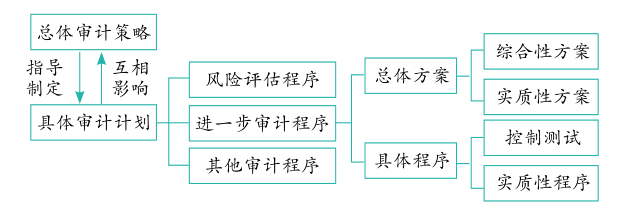
\includegraphics[width=0.7\linewidth]{screenshot001}
		\caption{}
		\label{fig:screenshot001}
	\end{figure}
	
	具体审计计划包括风险评估、计划实施的进一步审计程序和其他审计程序。其中其他审计程序的内容是考虑特殊事项的审计程序。
	
	确定审计程序的\textbf{性质、时间安排和范围}是具体审计计划的核心。详细的内容会在后续章节中展开
	
	\paragraph{审计过程中对计划的更改}
	计划审计工作贯穿于整个审计业务的始终,注册会计师应在必要时对总体审计策略和具体审计计划作出更新和修改。导致审计计划更改的事项有
	\begin{enumerate}
		\item 对\textbf{重要性水平}的修改
		
		\item 对\textbf{某类交易、账户余额和披露的重大错报风险评估}的更新和修改
		
		\item 对\textbf{进一步审计程序}(包括总体方案和拟实施的具体审计程序的更新和修改)
	\end{enumerate}
	
	\paragraph{指导、监督与复核}
	注册会计师应当制定计划,确定对项目组成员的指导、监督以及对其工作进行复核的性质、时间安排和范围,主要取决于下列因素:
	\begin{enumerate}
		\item 被审计单位的规模和复杂程度;
		
		\item 审计领域;
		
		\item 评估的重大错报风险;
		
		\item 执行审计工作的项目组成员的专业素质和胜任能力
	\end{enumerate}

	
	\subsection{重要性}
	\subsubsection{错报}
	重要性的本质是用来\textbf{衡量错报是否重大}。因此我们要首先分析什么是错报
	
	\paragraph{错报的定义与来源}
	错报指某一财务报表项目的金额、分类或列报,\textbf{与按适用的财务报告编制基础}应列示的金额、分类、列报之间\textbf{存在的差异};以及根据注册会计师的判断,为使财务报表在所有重大方面实现公允反映,需要对金额、分类、列报作出必要的调整。
	
	错报\textbf{来源于舞弊或错误}。主要分为以下几类
	\begin{enumerate}
		\item \textbf{事实错报}。收集或处理数据错误,对事实的误解或忽略,或故意舞弊行为。本质是\textbf{违反客观事实}
		
		\item \textbf{判断错报}。管理层和注册会计师\textbf{对会计估计值的判断差异};管理层和注册会计师对\textbf{选择和运用会计政策的判断差异}
		
		\item \textbf{推断错报}。通常指根据\textbf{样本推断的总体错报}
	\end{enumerate}
	
	\paragraph{错报的识别和更正}
	错报\textbf{可能不会孤立发生},一项错报的发生还可能表明存在其他错报。
		
	\textbf{抽样风险和非抽样风险可能导致某些错报未被发现}(相关概念在“审计抽样方法”章节详解)。审计过程中累积错报的汇总数接近确定的重要性,表明存在比可接受的低风险水平更大的风险,即可能未被发现的错报连同审计过程中累积错报的汇总数,可能超过重要性。
		
	通常,注册会计师应当及时将审计过程中累积的\textbf{所有错报与适当层级的管理层进行沟通,还应当要求管理层更正这些错报}。
	
	
	\subsubsection{重要性的概念}
	重要性的本质是用来\textbf{衡量错报是否重大}。在\textbf{制定总体审计策略}时需要确定重要性。
	
	重要性的判断维度主要是从\textbf{定量以及定性}两个方面进行判断。在定量层面,如果\textbf{错报金额超过财务报表整体的重要性},则错报通常是重大的。
	
	在定性层面,如果某些错报金额低于财报整体的重要性,并不说明错报不重大。某些错报金额高于财报整体的重要性,但是相对资产负债表占比较小,且对关键信息的披露不产生重大影响,则可能认定这样的错报不重大。
	
	
	重要性的概念包括以下系列:
	\begin{enumerate}
		\item \textbf{财务报表整体的重要性};
		
		\item \textbf{实际执行的重要性};
		
		\item \textbf{特定类别的交易、账户余额或披露的重要性};(某种情况下确定)
		
		\item \textbf{明显微小错报的临界值}
	\end{enumerate}

	
	在\textbf{计划和执行审计工作},\textbf{评价识别出的错报对审计的影响},以及\textbf{未更正错报对财务报表和审计意见的影响}\textbf{以上三个程序}时,注册会计师需要运用重要性概念。
	
	其中计划与执行审计工作可以具体分为\textbf{风险评估程序}与\textbf{进一步审计程序}。进一步审计程序又包括了控制测试与实质性程序(分为细节测试和实质性分析程序)
	
	\textbf{重要性的作用}一方面在于为注册会计师在计划审计工作时对何种情形构成重大错报作出的判断,也同时为下列方面提供了基础:
	\begin{enumerate}
		\item 确定风险评估程序的性质、时间安排和范围;
	
		\item 识别和评估重大错报风险;
	
		\item 确定进一步审计程序的性质、时间安排和范围
	\end{enumerate}
	
	\subsubsection{重要性的确定}
	考虑因素(1个自身2个财务报表)
	\begin{enumerate}
		\item 对被审计单位及其环境等方面情况的了解
		
		\item 财务报表个项目的性质及其相互关系
		
		\item 财务报表项目的金额及其波动幅度
	\end{enumerate}
	
	不考虑与具体项目相关的固有不确定性
	
	\paragraph{财务报表整体重要性}
	如果合理预期错报单独或连同其他错报可能影响财务报表使用者的决策,则该项错报是重大的。注册会计师通过执行审计工作对财务报表发表审计意见,因此应当考虑财务报表整体的重要性。

	具体方法:财务报表整体的重要性=基准×百分比,因此确定时只\textbf{考虑基准和百分比两个因素}。
	
	\textbf{选择基准的考虑因素}。包括:
	\begin{enumerate}
		\item 财务报表要素;(直接用作基准)
		
		\item 是否存在财务报表使用者特别关注的项目;(比如不同类型的公司用不同的项目)
		
		\item 被审计单位的性质、所处的生命周期阶段以及所处行业和经济环境;
		
		\item 被审计单位的所有权结构和融资方式;
		
		\item 基准的相对波动性。
	\end{enumerate}
	
	\textbf{选择基准的示例}如下
	\begin{enumerate}
		\item 企业的盈利水平保持稳定。\textbf{经常性业务的税前利润}
		
		\item 企业近年来经营状况大幅度波动,盈利和亏损交替发生,或由正常盈利变为微利或微亏,或本年度税前利润因情况变化而出现意外增加或减少
		
		\textbf{过去3~5年经常性业务的平均税前利润或亏损(取绝对值),或其他基准,例如营业收入}
		
		\item 国际企业集团设立的研发中心,主要为集团下属企业提供研发服务,并以成本加成方式向相关企业收取费用。\textbf{成本与营业费用总额}
		
		\item 企业为新设企业,处于开办期,尚未开始经营,目前正在建造厂房及购买机器设备。\textbf{总资产}
		
		\item 企业处于新兴行业,目前侧重于抢占市场份额、扩大知名度和影响力。\textbf{营业收入}
		
		\item 开放式基金,致力于优化投资组合、提高基金净值、为基金持有人创造投资价值。\textbf{净资产}
		
	\end{enumerate}
	
	
	\textbf{百分比的确定方法}(实务中通常为1\%~5\%)。考虑因素包括:
	\begin{enumerate}
		\item 是否为上市公司或公众利益实体;
		
		\item 财务报表使用者的范围;
		
		\item 被审计单位是否由集团内部关联方提供融资或是否有大额对外融资;
		
		\item 财务报表使用者是否对基准数据特别敏感等。
		
	\end{enumerate}
	
	\paragraph{特定类别的交易、账户余额或披露的重要性水平}
	特定类别的交易、账户余额或披露发生错报时,\textbf{即使错报金额低于财务报表整体的重要性},但如果能够合理预期该错报可能影响报表使用者依据财务报表作出的经济决策,应确定该认定的重要性水平。(在某种情况下才应当确定)
	
	确定该重要性的方法主要如下
	\begin{enumerate}
		\item 法律法规或适用的财务报告编制基础是否影响财务报表使用者对特定项目计量或披露的预期关联方交易、管理层和治理层的薪酬等
		
		\item 与被审计单位所处行业相关的关键性披露制药企业的研究与开发成本等
		
		\item 财务报表使用者是否特别关注财务报表中单独披露的业务的特定方面重大企业合并的披露等
	\end{enumerate}
	
	\textbf{实务操作上主要有两种情况}
	\begin{enumerate}
		\item 特定类别交易、账户余额或披露的重要性水平\textbf{应低于财务报表整体的重要性};
		
		\item \textbf{与财务报表整体的重要性相同},认定层次的重要性也需要相应确定实际执行的重要性。
	\end{enumerate}

	
	\paragraph{实际执行的重要性}
	
	实际执行的重要性,是指注册会计师确定的\textbf{低于财务报表整体重要性的一个或多个金额},旨在将\textbf{未更正和未发现错报的汇总数超过财务报表整体重要性的可能性降至适当的低水平};如果适用,还指注册会计师确定的低于特定类别的交易、账户余额或披露的重要性水平的一个或多个金额。
	
	在确定该重要性时主要考虑如下几个因素
	\begin{enumerate}
		\item 对被审计单位的了解;
		
		\item 前期审计工作中识别出的错报的性质和范围;
		
		\item 根据前期识别出的错报对本期错报作出的预期。
	\end{enumerate}
	
	实务操作上通常财务报表层次实际执行的重要性通常为财务报表\textbf{整体重要性的50\%~75\%}。根据不同情形进行变化。
	
	\begin{enumerate}
		\item 注册会计师在计划审计工作时可以根据实际执行的重要性确定需要对哪些类型的交易、账户余额和披露实施进一步审计程序,即通常选取金额超过实际执行的重要性的财务报表项目
		
		\item 不代表注册会计师可以对所有金额低于实际执行的重要性的财务报表项目不实施进一步审计程序,这是由于
		\begin{enumerate}
			\item 单个金额低于实际执行的重要性的财务报表项目汇总起来可能金额重大,注册会计师需要考虑汇总后的潜在错报风险;
			
			\item 对于存在低估风险的财务报表项目,不能仅仅因为其金额低于实际执行的重要性而不实施进一步审计程序;
			
			\item 对于识别出存在舞弊风险的财务报表项目,不能因为其金额低于实际执行的重要性而不实施进一步审计程序。
		\end{enumerate}
	\end{enumerate}

	
	\paragraph{明显微小错报的临界值}
	如果注册会计师将低于某一金额的错报界定为明显微小的错报,这些错报无论从规模、性质或其发生的环境,无论单独或者汇总起来,\textbf{都是明显微不足道的}。
	
	注册会计师应当在审计工作底稿中记录设定的明显微小错报临界值,低于该金额的错报视为明显微小的错报,\textbf{可以不累积}。
	
	“明显微小”不等同于“不重大”。如果不确定一个或多个错报是否明显微小,就不能认为这些错报是明显微小。
	
	在确定上,明显微小错报的临界值通常为财务报表\textbf{整体重要性的3\%至5\%,通常不超过10\%},除非注册会计师认为有必要单独为重分类错报确定一个更高的临界值。考虑因素如下
	\begin{enumerate}
		\item 以前年度审计中识别出的错报(包括已更正和未更正错报)的数量和金额;
		
		\item 重大错报风险的评估结果;
		
		\item 被审计单位治理层和管理层对注册会计师与其沟通错报的期望;
		
		\item 被审计单位的财务指标是否勉强达到监管机构的要求或投资者的期望。
		
	\end{enumerate}

	
	\subsubsection{审计过程中修改重要性}
	由于下列原因,注册会计师可能需要修改财务报表整体的重要性和特定类别的交易、账户余额或披露的重要性水平:
	\begin{enumerate}
		\item 审计过程中情况发生重大变化(如决定处置被审计单位的一个重要组成部分)
		
		\item 获取新信息
		
		\item 通过实施进一步审计程序,注册会计师对被审计单位及其经营所了解的情况发生变化
	\end{enumerate}
	
	
	
	
	
	\newpage
	\section{审计证据}	
	\subsection{审计证据的性质}
	审计证据是指注册会计师为了得出审计结论、形成审计意见而使用的所有信息。
	
	审计证据的所有信息是与审计过程相对应的概念。包括在\textbf{初步业务活动、审计测试流程、完成审计工作与出具审计报告}这几个过程中获得的审计证据。
	
	审计证据主要可以分为以下几类
	\begin{enumerate}
		\item 会计记录中含有的信息
		\begin{enumerate}
			\item 帐、证、表及其他调整
			
			\item 手工计算表和电子数据表等
		\end{enumerate}
		
		\item 其他的信息
		\begin{enumerate}
			\item 从内部或外部获取的会计记录以外的信息
			
			\item 通过询问、观察和检查等程序获取的信息
			
			\item 自身编制或获取的可以通过合理推断得出结论的信息
		\end{enumerate}
	\end{enumerate}
	
	上述两者缺一不可,没有前者,审计工作无法进行;没有后者,可能无法识别重大错报风险。
	
	审计证据主要考虑两个性质,\textbf{充分性与适当性}。一个代表量一个代表质。质可以影响量,反之不行。适当性中,只有\textbf{相关且可靠}的审计证据才是高质量的。
	\begin{enumerate}
		\item \textbf{相关性}指的是用作审计证据的信息与审计程序的目的和所考虑的相关认定之间的逻辑联系。
		
		\item 审计证据的\textbf{可靠性}收到其来源和性质的影响,并取决于获取审计证据的具体环境。
	\end{enumerate}
	
	评价审计证据时还有以下几个特殊考虑
	\begin{enumerate}
		\item 对文件记录可靠性的考虑
		
		\item 使用被审计单位生成信息时的考虑
		
		\item 证据相互矛盾时的考虑
		
		\item 获取审计证据时对成本的考虑
	\end{enumerate}
	
	\subsection{审计程序}
	基本的审计程序包括了\textbf{检查、观察、询问、函证、重新计算、重新执行和分析}。这些基本的审计程序组合起来也可以形成其他的审计程序。
	
	在审计测试流程过程中,不同的阶段(程序)会使用不同的审计程序。
	\begin{enumerate}
		\item 风险评估程序:检查、观察、询问、分析程序
		
		\item 控制测试(进一步审计程序):检查、观察、询问、重新执行
		
		\item 实质性程序中的细节测试(进一步审计程序):细节测试使用检查、观察、询问、函证、重新计算
		
		\item 实质性程序中的实质性分析程序(进一步审计程序):实质性分析程序使用分析程序
	\end{enumerate}
	
	其中检查分为正查和逆查
	
	\subsection{函证}
	函证相关的内容主要考虑如下的因素
	\begin{enumerate}
		\item 函证决策
		
		\item 函证设计
		
		\item 函证发出
		
		\item 函证收回与否,以及函证过程中设计的舞弊风险迹象的应对措施
	\end{enumerate}
	
	\subsubsection{函证决策}
	函证决策的考虑因素可以分为应当考虑和可以考虑两类,\textbf{应当考虑}的因素如下
	\begin{enumerate}
		\item 评估的认定层次重大错报风险
		
		\item 函证程序针对的认定
		
		\item 实施除函证以外其他的审计程序
	\end{enumerate}
	
	可以考虑的因素如下
	\begin{enumerate}
		\item 被询证者对函证事项的了解
		
		\item 预期被询证者恢复询证函的能力或意愿
		
		\item 预期被询证者的客观性
	\end{enumerate}
	
	函证的对象主要两个,一个是银行存款、借款及与金融机构往来的其他重要信息,另一个是应收账款。
	
	函证时间上通常\textbf{以资产负债表日为截止日},在资产负债表日后适当时间实施函证。如果重大错报风险评估为低水平,可选择资产负债表日前适当日期为截止日实施函证,并对资产负债表日前发生的变动实施实质性程序。
	
	管理层要求不实施函证,如果要求合理,则实施替代程序。如果要求不合理且被管理层阻挠无法实施函证,则视为审计范围受到限制,并考虑对审计报告可能产生的影响。
	
	\subsubsection{函证设计}
	需要根据特定审计目标设计询证函。针对存在和完整性认定,有着不同的函证方式。
	
	设计询证函时,以下的因素会影响函证的可靠性
	\begin{enumerate}
		\item 函证的方式。分为积极式函证与消极式函证
		
		\item 以往审计或类似业务的经验
		
		\item 拟函证信息的性质
		
		\item 选择被询证者的适当性
		
		\item 被询证者易于回函的信息类型
	\end{enumerate}
	
	\subsubsection{函证发出}
	注册会计师应当对函证的全过程保持控制。
	
	发出方式有以下几种:邮寄、跟函、电子形式。
	
	第三方电子询证函平台可能导致回函不可靠的风险有以下几种:独立性风险、安全性风险。
	
	\subsubsection{函证收回与否}
	函证可能受到回函也可能未受到回函。
	
	如果受到回函,则需要判断回函的可靠性。主要考虑因素有如下几点
	\begin{enumerate}
		\item 对询证函的设计、发出及收回的控制情况
		
		\item 被询证者的胜任能力、独立性、授权回函情况、对函证项目的了解及其客观性
		
		\item 被审计单位施加的限制或回函中的限制
	\end{enumerate}
	
	回函中\textbf{可能会出现影响回函可靠性的限制性条款},通常应对措施如下
	\begin{enumerate}
		\item 可能需要执行额外的或替代审计程序,若不可行,确定其对审计工作和审计意见的影响
		
		\item 在特殊情况下,注册会计师可能要求被询证者澄清或寻求法律意见
	\end{enumerate}
	
	如果函证中存在不符事项,注册会计师应当调查不符事项,确定是否表明存在错报或者舞弊。
	
	如果在合理的时间内未收到积极式询证函的回函,注册会计师应当考虑必要时再次发出询证函,如果仍未收到回函,应当实施替代程序。
	
	\subsubsection{舞弊风险}
	
	可能出现舞弊风险的现象,针对舞弊风险迹象注册会计师可以采取的应对措施
	
	\subsection{分析程序}
	分析程序主要针对的是财务信息,考虑的关系包括财务信息之间以及财务信息和非财务信息之间的关系。形成的预期值包括
	\begin{enumerate}
		\item 以前期间的可比信息
		
		\item 审计客户的预期结果
		
		\item 注册会计师的预期数据,如折旧的估计值
		
		\item 可比的行业信息
	\end{enumerate}
	
	分析程序\textbf{应当用在风险评估程序与总体复核,可以用于实质性程序}。
	
	\subsubsection{用作风险评估}
	了解被审计单位及其环境等方面情况,并评估财务报表重大错报风险。主要目的在于识别可能表明\textbf{财务报表存在重大错报风险的异常变化}。
	
	\subsubsection{用作实质性程序}
	实质性程序包括细节测试与实质性分析程序。
	
	当\textbf{使用分析程序比细节测试能更有效地将认定层次的检查风险降低至可接受的水平}时,注册会计师可以考虑单独或结合细节测试运用实质性分析程序。这样可以减少细节测试的工作量。某些时候也可以单独使用实质性分析程序。
	
	但是实质性分析程序并不适用于所有的财务报表认定。与细节测试相比,实质性分析程序能够达到的精确度可能受到种种限制,所提供的证据在很大程度上是间接证据,证明力相对较弱。
	
	在用作实质性程序时,需要考虑如下的因素
	\begin{enumerate}
		\item 对特定认定的适用性
		
		\item 数据的可靠性
		
		\item 评价预期值的准确程度
		
		\item 对可接受的差异额的考虑
	\end{enumerate}
	
	
	\subsubsection{用作总体复核}
	在临近审计结束时对财务报表进行总体复核(集中在财务报表层次),考虑是否需要追加审计程序
	
	和风险评估程序中使用的分析程序手段基本相同,但是目的不同。两者主要的区别在于实施分析程序的时间和重点不同,以及所去的的数据的数量和质量不同。
	
	\newpage
	\section{审计抽样方法}
	\subsection{审计抽样的相关概念}
	\subsubsection{审计抽样的含义}
	审计抽样是选取项目的一种方式,选取项目总共有三种方法
	\begin{enumerate}
		\item 全查:对某总体包含的全部项目进行测试
		
		\item 特定项目检查:对选出的特定项目进行测试,但不推断总体
		
		\item 抽样检查:审计抽样,以样本结果推断总体结论。
	\end{enumerate}
	
	具体来说,审计抽样就是注册会计师对具有审计相关性的总体中低于百分之百的项目实施审计程序,使所有抽样单元均有被选取的机会,为注册会计师针对整个总体得出结论提供合理的基础
	
	审计抽样有着如下的基本特征
	\begin{enumerate}
		\item 对具有审计相关性的总体中低于百分之百的项目实施审计程序,即全查不属于审计抽样
		
		\item 所有抽样单元都有被选取的机会(但不意味着所有抽样单元都应有均等的机会)
		
		\item 可以根据样本项目的测试结果推断出有关抽样总体的结论。(样本代表性)
	\end{enumerate}
	
	代表性,是指在既定的风险水平下,注册会计师根据样本得出的结论,与对整个总体实施与样本相同的审计程序得出的结论类似;只有当从抽样总体中选取的样本具有代表性时,注册会计师才能根据样本项目的测试结果推断出有关总体的结论。代表性和样本整体、错报的发生率、如何选取样本有关。
	
	审计抽样主要用于两个环节,一个是有运行轨迹的控制测试(除信息技术控制),另一个是实质性程序中的细节测试。
	
	\subsubsection{审计抽样的类型}
	对审计抽样进行分类,我们可以从两个纬度进行。

	\begin{table}[h!]
		\centering
		\caption{统计抽样与非统计抽样}
		\begin{tblr}{
				width = \linewidth,
				colspec = {Q[50]Q[465]Q[425]},
				cell{4}{2} = {c=2}{0.89\linewidth},
				hlines,
				vlines,
			}
			类型 & 统计抽样                                          & 非统计抽样                                    \\
			定义 & 同时具备两个特征:
			(1)随机选取样本项目;
			(2)运用概率论评价样本结果、
			计量抽样风险 & 不同时具备两个特征                                \\
			特点 & (1)客观计量抽样风险;
			(2)成本较高                          & (1)无法计量抽样风险;
			(2)如果设计适当,也能提供与统计抽
			样同样有效的结果 \\
			决策 & 注册会计师在统计抽样与非统计抽样方法之间进行选择时主要考虑成本效
			益,并运用职业判断    &                                          
		\end{tblr}
	\end{table}
	
	
	\begin{table}[h!]
		\centering
		\caption{属性抽样与变量抽样}
		\begin{tblr}{
				width = \linewidth,
				colspec = {Q[60]Q[527]Q[354]},
				hlines,
				vlines,
			}
			类型 & 属性抽样                     & 变量抽样             \\
			定义 & 对总体中某一事件发生率得出结论的统
			计抽样方法  & 对总体金额得出结论的统计抽样方法 \\
			运用 & 控制测试                     & 细节测试             \\
			目的 & 测试某一设定控制的偏差率,而不考虑交易的金额大小 & 确定记录金额是否         
		\end{tblr}
	\end{table}
	
	\subsubsection{具体的选样方法}
	选样方法通常有以下几种
	\begin{enumerate}
		\item 简单随意选样。相同数量的抽样单元组成的每种组合被选取的概率都相等;可以使用计算机或随机数表
		
		\item 系统选样
		\begin{enumerate}
			\item 确定选样间隔:选样间隔= 总体数量/样本规模
			
			\item 确定随机起点,按照选样间隔,顺序选取样本
			
			\item 总体中的每一个抽样单元被选取的机会都相等
			
			\item 总体必须是随机排列的
		\end{enumerate}
		
		\item 随意选样。注册会计师要避免任何有意识的偏向或可预见性,保证总体中的所有项目都有被选中的机会; 无法量化选取样本的概率
		
		\item 整群选样。从总体中选取一群(或多群)连续的项目; 通常不能在审计抽样中使用
	\end{enumerate}
	
	统计抽样可以使用简单随意选样和系统选样;非统计抽样可以使用简单随意选样、系统选样和随意选样。
	
	\subsubsection{抽样风险和非抽样风险}
	\paragraph{抽样风险}
	抽样风险是指根据样本得出的结论,可能不同于如果对整个总体实施与样本相同的审计程序得出的结论的风险。
	
	抽样风险由抽样引起,与样本规模和抽样方法相关。样本规模越大,抽样风险越小。如果对所有项目都实施检查,则不存在抽样风险。
	
	控制测试中有两种风险:信赖过度风险与信赖不足风险。细节测试中也有两种风向:误拒风险和误受风险。
	
	误受风险和信赖过度风险都会影响效果。误拒风险和信赖不足风险则都会影响效率。
	
	\paragraph{非抽样风险}
	非抽样风险指由于任何与抽样风险无关的原因而得出错误结论的风险。(人为因素)
	
	实施控制测试和实质性程序时均可能产生非抽样风险。非抽样风险是由人为因素造成的,难以量化
	
	可以降低或防范,即可以通过仔细设计审计程序,采取适当的质量管理政策和程序,对 审计工作进行适当的指导、监督和复核,适当改进实务工作,\textbf{将非抽样风险降至合理保证的可接受的水平}。
	
	\subsection{审计抽样在控制测试中的应用}
	在控制测试和细节测试中,审计抽样都有着以下的三个大环节
	\begin{enumerate}
		\item 设计样本阶段
		
		\item 选取样本阶段
		
		\item 评价样本结果阶段
	\end{enumerate}
	每个大环节中细分的小环节则各有着不同
	
	\subsubsection{设计样本阶段}
	\paragraph{确定测试目标} 注册会计师实施控制测试的目标是提供关于控制运行有效性的审计证据,以支持计划的重大错报风险评估水平。
	
	\paragraph{定义总体和抽样单元}
	定义总体需要考虑以下三个因素
	\begin{enumerate}
		\item 适当性。总体适合于特定的审计目标
		
		\item 完整性。应当从总体项目内容和涉及时间等方面确定总体的完整性
		
		\item 同质性。总体中的所有项目应该具有同样的特征; 评价不同的控制情况,定义不同的独立主体; 在本期发生重大变化的内部控制,应针对变化前后分别定义总体
	\end{enumerate}
	
	注册会计师定义的抽样单元应与审计测试目标相适应。抽样单元通常是能够提供控制运行证据的一份文件资料、一个记录或其中一行,每个抽样单元构成了总体中的一个项目。
	
	\paragraph{定义偏差构成条件} 在控制测试中,偏差是指偏离对设定控制的预期执行。在评估控制运行的有效性时,注册会计师应当考虑其认为必要的所有控制环节。
	
	\paragraph{定义测试期间} 注册会计师通常在期中实施控制测试,由于期中测试获取的证据只与控制截至期中测试 时点的运行有关,注册会计师需要确定如何获取关于剩余期间的证据。
	
	\subsubsection{选取样本阶段}
	\paragraph{确定抽样方法} 注册会计师运用职业判断选择统计抽样或非统计抽样。
	
	\paragraph{确定样本规模} 影响样本规模的主要因素有
	\begin{enumerate}
		\item 可接受的信赖过度风险
		
		\item 可容忍偏差率。最高20\%
		
		\item 预计总体偏差率
		
		\item 总体规模。影响很小
	\end{enumerate}
	
	在具体确定样本量时,如果是非统计抽样则运用职业判断确定样本规模;如果是统计抽样,则根据统计公式确定样本规模。
	
	\paragraph{选取样本并实施审计程序} 如果能够合理确信该无效单据是正常的且不构成设定控制的偏差, 则可以用另外的单据替代; 如果使用随机选样,要用一个替代的随机数与新的单据样本对应
	
	注册会计师应当针对选取的每个项目,实施适合于具体审计目标的审计程序; 如果注册会计师\textbf{无法对选取的项目实施计划的审计程序或适当的替代程序}(例如,单据丢失或损毁),考虑在评价样本时将该样本项目视为控制偏差
	
	\subsubsection{评价样本结果阶段}
	\paragraph{计算偏差率} 将样本中发现的偏差数量除以样本规模,就可以计算出样本偏差率。样本偏差率就是注 册会计师对总体偏差率的最佳估计,因而在控制测试中无须另外推断总体偏差率。但注册会计师还必须考虑抽样风险。
	
	\paragraph{考虑抽样风险}
	统计抽样和非统计抽样有着不同的抽样风险考虑方法。
	\begin{table}[h!]
		\centering
		\caption{统计抽样}
		\begin{tblr}{
				width = \linewidth,
				colspec = {Q[217]Q[146]Q[577]},
				cell{1}{1} = {c=2}{0.363\linewidth},
				cell{2}{1} = {r=2}{},
				cell{4}{1} = {r=3}{},
				vlines,
				hline{1-2,4,7} = {-}{},
				hline{3,5-6} = {2-3}{},
			}
			情形         &        & 关键要点                       \\
			计算偏差率上限    & 统计公式法  & 总体偏差率上限=风险系数(R)/样本量(n)     \\
			& 查表法    & 注册会计师也可以使用样本结果评价表读取总体偏差率上限 \\
			判断总体
			是否可接受 & 可以接受   & 低于          \\
			& 不能接受   & 大于或等于  \\
			& 考虑是否接受 & 低于但接近  
		\end{tblr}
	\end{table}
	
	在非统计抽样中,抽样风险无法直接计量,注册会计师通常将估计的总体偏差率(即样本偏差率)与可容忍偏差率相比较,以判断总体是否可以接受。
	
	\begin{table}[h!]
		\centering
		\caption{非统计抽样}
		\begin{tblr}{
				width = \linewidth,
				colspec = {Q[181]Q[108]Q[650]},
				cell{1}{1} = {c=2}{0.289\linewidth},
				cell{2}{1} = {r=3}{},
				vlines,
				hline{1-2,5} = {-}{},
				hline{3-4} = {2-3}{},
			}
			情形         &       & 关键要点                                     \\
			判断总体
			是否可接受 & 可以接受  & 大大低于                  \\
			& 不能接受  & 1大于或等于
			2低于但接近\\
			& 进一步测试 & 差异不大不小                
		\end{tblr}
	\end{table}
	
	\paragraph{考虑偏差的性质和原因}
	注册会计师有两种处理办法: 
	\begin{enumerate}
		\item 扩大样本规模,以进一步收集证据;但是,如果确定控制偏差是系 统偏差或舞弊导致,扩大样本规模通常无效
		
		\item 认为控制没有有效运行,样本结果不支持计划的控制运行有效性和 重大错报风险的评估水平,因而提高重大错报风险评估水平,增加对相关 账户的实质性程序
	\end{enumerate}
	
	\paragraph{得出总体结论}
	如果样本结果不支持计划的控制运行有效性和重大错报风险的评估水平,注册会计师通常有两种选择:
	\begin{enumerate}
		\item 进一步测试其他控制(如补偿性控制),以支持计划的控制运行有效性和重大错报风险的评估水平;
		
		\item 提高重大错报风险评估水平,并相应修改计划的实质性程序的性质、时间安排和范围。
	\end{enumerate}
	
	
	
	\subsection{审计抽样在细节测试中的应用}
	
	\subsubsection{设计样本阶段}
	\paragraph{确定测试目标} 在细节测试中,审计抽样通常用来测试有关财务报表金额的一项或多项认定的合理性。
	
	\paragraph{定义总体} 考虑两个因素
	\begin{enumerate}
		\item 适当性
		
		\item 完整性
	\end{enumerate}
	
	\paragraph{定义抽样单元}
	抽样单元可能是一个账户余额、一笔交易或交易中的一个记录,甚至是每个货币 单元;注册会计师定义抽样单元时应考虑实施计划的审计程序或替代程序的难易程度
	
	\paragraph{界定错报}
	注册会计师应根据审计目标界定错报
	
	\subsubsection{选取样本阶段}
	\paragraph{确定抽样方法}
	这里主要考虑统计抽样中的传统变量抽样和货币单元抽样
	
	传统变量抽样主要有
	\begin{enumerate}
		\item 均值法
		
		\item 差额法
		
		\item 比率法
	\end{enumerate}
	
	货币单元抽样运用属性抽样原理,对货币金额而不是对发生率得出结论的统计抽样方 法,是概率比例规模抽样方法的分支,也称为金额单元抽样、累计货币金 额抽样以及综合属性变量抽样。抽样单元是货币单元。
	
	\begin{table}[h!]
		\centering
		\begin{tblr}{
				width = \linewidth,
				colspec = {Q[94]Q[417]Q[429]},
				hlines,
				vlines,
			}
			纬度    & 传统变量抽样                        & 货币单元抽样                        \\
			理论基础  & 变量抽样                          & 属性抽样                          \\
			复杂度   & 复杂                            & 比传统变量抽样更易于使用                  \\
			适用性   & 可以用于测试低估                      & 不适用于测试低估                      \\
			抽样风险  & 高估抽样风险的影响较小                   & 可能高估抽样风险的影响,导致拒绝
			一个可接受的总体账面金额 \\
			设计样本  & 难                             & 易                             \\
			选取样本  & 无须特别考虑零余额或负余额~ ~ ~ ~ ~ ~ ~ ~~ & 需要特别考虑零余额或负余额~ ~ ~ ~ ~ ~ ~ ~~ \\
			考虑变异性 & 需要考虑                          & 无须考虑                          \\
			分层要求  & 需要考虑                          & 无须分层                          \\
			样本规模  & 预计错报不存在时,样本规模更
			大;预计错报多,样本规模更小 & 预计错报不存在时,样本规模更小;
			预计错报多,样本规模更大 
		\end{tblr}
	\end{table}
	
	\paragraph{确定样本规模}
	影响样本规模的主要因素有
	\begin{enumerate}
		\item 可接受的误受风险
		
		\item 可容忍偏差率。最高20\%
		
		\item 预计总体错报
		
		\item 总体规模。影响很小
		
		\item 总体的变异性
	\end{enumerate}
	
	具体的样本量确定上,统计抽样用计算机确定样本规模,非统计抽样用经验公式:样本规模= 总体账面金额/可容忍错报 ×保证系数
	
	\paragraph{选取样本并实施审计程序}注册会计师应对选取的每一个样本实施适合于具体审计目标的审计程序。无法对选取的项目实施检查时,注册会计师应当考虑这些未 检查项目对样本评价结果的影响
	
	\subsubsection{评价样本结果阶段}
	\paragraph{推断总体的错报}
	如果注册会计师在设计样本时将进行抽样的项目分为几层,则要在每层分别推断 错报,然后将各层推断的金额加总,计算估计的总体错报。注册会计师还要将在进行百分之 百检查的个别重大项目中发现的所有错报与推断的错报金额汇总。
	
	使用货币单元抽样时,需要注意基本原理,即每一个被选取的货币单元都代表了 整个选样间隔中所有的货币单元。根据逻辑单元的类型,可以使用不同的推断方法,如下表 所示。
	\begin{enumerate}
		\item 大单元,逻辑单元账面金额≥选样间隔。推断的错报=逻辑单元的实际错报
		
		\item 小单元,逻辑单元账面金额<选样间隔。先计算错报的百分比,错报百分比=(样本账面金额-样本审定金额)/ 样本账面金额。推断的错报=错报百分比×选样间隔
		
	\end{enumerate}
	
	\paragraph{考虑抽样风险}
	非统计抽样中注册会计师运用职业判断和经验考虑抽样风险
	
	
	\begin{table}[h!]
		\centering
		\begin{tblr}{
				width = \linewidth,
				colspec = {Q[379]Q[235]Q[308]},
				cell{1}{1} = {c=2}{0.614\linewidth},
				cell{2}{1} = {r=3}{},
				vlines,
				hline{1-2,5} = {-}{},
				hline{3-4} = {2-3}{},
			}
			情形         &        & 关键要点     \\
			判断总体是否可以接受 & 可以接受   & 远远低于     \\
			& 不能接受   & 大于或接近或等于 \\
			& 考虑是否接受 & 差距不大不小   
		\end{tblr}
	\end{table}
	
	统计抽样中以总体错报上限为基础判断。基本精确度+事实错报+每一推断错报×相应的保证系 数的增量
	
	\begin{table}[h!]
		\centering
		\begin{tblr}{
				width = \linewidth,
				colspec = {Q[463]Q[198]Q[242]},
				cell{1}{1} = {c=2}{0.661\linewidth},
				cell{2}{1} = {r=2}{},
				vlines,
				hline{1-2,4} = {-}{},
				hline{3} = {2-3}{},
			}
			情形         &      & 关键要点  \\
			判断总体是否可以接受 & 可以接受 & 小于    \\
			& 不能接受 & 大于或等于 
		\end{tblr}
	\end{table}
	
	
	\paragraph{考虑错报的性质和原因}
	除了评价错报的金额和频率以及抽样风险之外,注册会计师还应当考虑: 错报的性质和原因;错报与审计工作其他阶段之间可能存在的关系。
	
	\paragraph{得出总体结论}
	(1)如果样本结果不支持总体账面金额,且注册会计师认为账面金额可能存在错报,
	注册会计师通常会建议被审计单位对错报进行调查,并在必要时调整账面记录。
	
	(2)依据被审计单位已更正的错报对推断的总体错报额进行调整后,注册会计师应当 将该类交易或账户余额中剩余的推断错报与其他交易或账户余额中的错报总额累计起来,以
	评价财务报表整体是否存在重大错报。 
	
	(3)无论样本结果是否表明错报总额超过了可容忍错报,注册会计师都应当要求被审
	计单位的管理层记录已发现的事实错报(除非低于明显微小错报临界值)。
	
	
	\newpage
	\section{信息技术对审计的影响}
	\subsection{信息技术对企业财务报告和内部控制的影响}
	
	\subsection{信息技术一般控制、信息处理控制和公司层面信息技术控制}、
	
	\subsection{信息技术对审计过程的影响}
	信息技术对审计产生的影响主要包括以下几个事项
	\begin{enumerate}
		\item 审计线索
		
		\item 审计技术手段
		
		\item 内部控制
		
		\item 审计内容
		
		\item 注册会计师
	\end{enumerate}
	
	\subsection{计算机辅助审计技术和电子表格的应用}
	\paragraph{计算机辅助审计技术}
	1.类型
	(1)面向系统的计算机辅助审计技术,包括平行模拟法、测试数据法、嵌入审计模块 法、程序编码审查、程序代码比较和跟踪、快照等方法;
	(2)面向数据的计算机辅助审计技术,包括数据查询、账表分析、审计抽样、统计分 析、数值分析等方法。
	2.应用
	计算机辅助审计技术的应用领域包括实质性程序(特别是分析程序)、控制测试以及辅 助对舞弊的检查等。
	
	\paragraph{电子表格}
	\begin{enumerate}
		\item 注册会计师应当了解评估范围内重要的流程和账户,并识别用来支持这些流程或账户的相关电子表格或工具。
		
		\item 电子表格(如Excel等软件)面临的固有风险和错误包括输入错误、逻辑错误、接口错误和其他错误等。
		
		\item 注册会计师应当了解相关的电子表格控制,包括: 
		\begin{enumerate}
			\item 对电子表格执行的、类似于信息系统一般控制的控制; 
			
			\item 内嵌在电子表格中的控制(类似于一个自动化信息处理控制); 
			
			\item 针对电子表格数据输入和输出的人工控制。
		\end{enumerate}
	\end{enumerate}
	
	\subsection{数据分析}
	
	\subsection{不同信息技术环境下的信息管理}
	
	\newpage
	\section{审计工作底稿}
	
	\subsection{审计工作底稿概述}
	\paragraph{基本概念}审计工作底稿是注册会计师对审计计划、审计程序、审计证据和审计结论的记录,\textbf{是审计证据的载体};审计工作底稿也可用于项目质量复核、监督会计师事务所以及第三方检查等。可能以纸质、电子或其他介质形式存在。审计工作底稿\textbf{形成于审计过程,反映整个审计过程}。
	
	主要内容包括了
	\begin{enumerate}
		\item 总体审计策略、具体审计计划
		
		\item 分析表、问题备忘录、重大事项概要
		
		\item 询证函回函的声明、核对表、有关重大事项的往来函件(包括电子邮件)
		
		\item 被审计单位文件记录的摘要或复印件
		
		\item 业务约定书、管理建议书、项目组内部或项目组与被审计单位举行的会议记录、与其他人士的沟通文件及错报汇总
	\end{enumerate}
	
	具体需要了解\textbf{不包括的内容}
	\begin{enumerate}
		\item 已被取代的审计工作底稿的草稿或财务报表的草稿(草拟的)
		
		\item 反映不全面或初步思考的记录(初级的)
		
		\item 存在印刷错误或其他错误而作废的文本(错误的)
		
		\item 重复的文件记录等(重复的)
	\end{enumerate}
	
	但是对审计计划、重要性的更新和修改的相关记录需要保存,不能删去
	
	\paragraph{目的}
	基本目的是
	\begin{enumerate}
		\item 提供充分、适当的记录,作为出具审计报告的基础
		
		\item 提供证据,证明已按照审计准则和法律法规的规定计划和执行了审计工作(即提高职业判断的可辩护性)
	\end{enumerate}
	
	\paragraph{编制要求}
	基本要求是应当使未曾接触该项审计工作的有经验的专业人士清楚地了解
	\begin{enumerate}
		\item 程序:按照规定实施的审计程序的性质、时间安排和范围
		
		\item 证据:实施审计程序的结果和获取的审计证据
		
		\item 结论:遇到的重大事项和得出的结论,以及作出的重大职业判断
	\end{enumerate}
	
	\paragraph{控制}
	无论审计工作底稿以哪种形式存在,会计师事务所都应当针对审计工作底稿设计和实施适当的控制,以实现下列目的
	\begin{enumerate}
		\item 清晰地显示其生成、修改及复核的时间和人员
		
		\item 在审计业务的所有阶段,尤其是在项目组成员共享信息或通过互联网传递信息时,\textbf{保护信息的完整性和安全性};
		
		\item 防止未经授权\textbf{改动审计工作底稿}
		
		\item 允许项目组和其他经授权的人员为适当履行职责而\textbf{接触审计工作底稿}
	\end{enumerate}
	
	\subsection{审计工作底稿的格式、要素和范围}
	确定审计工作底稿的格式、要素和范围时考虑的要素包括
	\begin{enumerate}
		\item 被审计单位的规模和复杂程度;
		
		\item 拟实施审计程序的性质;
		
		\item 识别出的重大错报风险;
		
		\item 已获取审计证据的重要程度;
		
		\item 识别出的例外事项的性质和范围
		
		\item 当从已执行工作或获取证据的记录中不易确定结论或结论的基础时,记录结论或结论基础的必要性
		
		\item 审计方法和使用的工具。
	\end{enumerate}
	
	审计工作底稿的要素包括以下八个
	\begin{enumerate}
		\item 审计工作底稿的标题
		
		\item 审计过程记录(重点)
		
		\item 审计结论
		
		\item 审计标识及其说明
		
		\item 索引号及编号
		
		\item 编制人员姓名及编制日期
		
		\item 复核人员姓名及复核日期
		
		\item 其他应说明的事项
	\end{enumerate}
	
	审计过程记录中有两个要点,一个是\textbf{识别特征},另一个是\textbf{重大事项}。
	
	\textbf{识别特征}是指被测试项目或事项表现出的征象或标 志。识别特征通常具有唯一性,可以使其他人员根据识别特征识别该项目或事项,并重新执行该测试。
	
	重大事项包括以下内容
	\begin{enumerate}
		\item 引起\textbf{特别风险}的事项
		
		\item 实施审计程序的结果表明财务信息\textbf{可能存在重大错报},或需要修正以前对重大错报风险的评估和拟采取的应对措施
		
		\item 导致注册会计师\textbf{难以实施必要审计程序}的情形
		
		\item 导致出具\textbf{非无保留意见}、带强调事项段或者“与持续经营相关的重 大不确定性”等段落的审计报告事项
	\end{enumerate}
	
	如果识别出的信息与针对某重大事项得出的最终结论不一致,注册会 计师应当记录如何处理不一致的情况
	
	\subsection{审计工作底稿的归档}
	归档,指将审计工作底稿归整为最终档案,属于一项事务性工作,不涉及实施新的审计 程序或得出新的审计结论。归档期间对审计工作底稿可以进行的变动如下
	\begin{enumerate}
		\item 除或废弃被取代的审计工作底稿
		
		\item 对审计工作底稿进行分类、整理和交叉索引
		
		\item 对审计档案归整工作的完成核对表签字认可
		
		\item 记录在审计报告日前获取的、与项目组相关成员进行讨论并达成一致意见的审计证据
	\end{enumerate}
	
	归档期限上,如果完成审计业务,审计报告日后60天内。如果未完成审计业务,审计业务中止后60天内
	
	审计底稿归档后可能出现了新的信息或者之前的记录不充分,这时需要变动审计工作底稿。注册会计师应当记录下列事项
	\begin{enumerate}
		\item 修改或增加审计工作底稿的理由、时间和人员
	
		\item 复核的时间和人员
	\end{enumerate}
	
	在审计底稿的保存上,会计师事务所应当自审计报告日起,对审计工作底稿至少保存10年。如果注册会计师未能完成审计业务,会计师事务所应当自业务中止日起,对审计 工作底稿至少保存10年。
	
	\newpage
	\section{风险评估}
	第七和第八章共同构成了风险导向审计测试流程,其核心是重大错报风险的识别、评估及应对。
	
	注册会计师通过实施风险评估程序,了解被审计单位及其环境等方面情况,识别和评估财务报表层次和认定层次的重大错报风险,为设计和实施总体应对措施和进一步审计程序,应对评估的重大错报风险提供依据。
	\subsection{风险识别和评估概述}
	风险评估主要为注册会计师在下列关键环节做出职业判断提供了重要基础
	\begin{enumerate}
		\item 确定重要性水平,并随着审计工作的进程评估对重要性水平的判断是否仍然适当
		
		\item 考虑会计政策的选择和运用是否恰当,以及财务报表的列报是否适当
		
		\item 识别与财务报表中金额或披露相关的需要特别考虑的领域,包括关联方交易、管理层运用持续经营假设的合理性,或交易是否具有合理的商业目的
		
		\item 确定在实施分析程序时所适用的预期只
		
		\item 设计和实施进一步审计程序,以将审计风险降至可接受的低水平
		
		\item 评价所获取审计证据的充分性与适当性
	\end{enumerate}
	
	风险评估与识别有着以下的要求
	\begin{enumerate}
		\item 贯穿审计过程
		
		\item 运用职业判断
		
		\item 预期的变化
		
		\item 评价了解程序
		
		\item 了解程度低于管理层
	\end{enumerate}
	
	
	\subsection{风险评估程序、信息来源以及项目组内部的讨论}
	风险评估程序是指注册会计师为识别和评估财务报表层次以及认定层次的重大错报风险而设计和实施的审计程序。
	
	注册会计师在设计与实施风险评估程序时,不应当偏向于获取佐证性的审计证据,也不应当排斥相矛盾的审计证据。
	
	风险评估主要了解三方面的内容
	\begin{enumerate}
		\item 了解被审计单位及其环境等方面。其中这一块的内容可以展开为三层。
		
		\item 了解适用的财务报告编制基础
		
		\item 了解内部控制体系要素
	\end{enumerate}
	
	所实施的程序包括询问、观察、检查、分析与穿行测试。其中前三项可以用于两个方面,分析主要用于了解被审计单位及其环境等方面,穿行测试主要用于了解内部控制体系要素。
	
	
	
	\subsection{了解被审计单位及其环境的和适用的财务报告编制基础}
	了解被审计单位及其环境时,主要了解以下三个方面
	\begin{enumerate}
		\item 组织结构、所有权和治理结构、业务模式
		
		\item 行业形式、法律环境、监管环境和其他外部因素
		
		\item 财务业绩的衡量标准,包括内部和外部使用的衡量标准
	\end{enumerate}
	
	注册会计师应当了解适用的财务报告编制基础、会计政策及变更会计政策的原因,并评价被审计单位的会计政策是否适当、是否与适用的财务报告编制基础一致。
	
	\subsection{了解被审计单位内部控制体系各要素}
	内部控制体系是指由治理层、管理层和其他人员设计、执行和维护的体系,以合理保证白审计单位能够实现财务报告的可靠性,提高经营效率和效果,以及遵守适用的法律法规等目的。
	
	具体来说,在COSO体系下包含以下五个要素
	\begin{enumerate}
		\item 内部环境(控制环境)
		
		\item 风险评估
		
		\item 内部监督
		
		\item 信息与沟通(信息系统与沟通)
		
		\item 控制活动
	\end{enumerate}
	值得注意的是其中的风险评估是企业内部自己执行的风险评估,并不是注册会计师执行的风险评估程序。
	
	其中内部环境、风险评估、内部监督是被审计单位内部控制体系的基础,其运行中的任何缺陷都可能对财务报表的编制产生广泛的影响。因此,注册会计师我对这些要素的了解和评估及,更有可能影响其对财务报表层次重大错报风险的识别和评估,也可能影响对认定层次重大错报风险的识别和评估。
	
	注册会计师需要了解和评价的内部控制只是与财务报表审计相关的内部控制,并非被审计单位所有的内部控制。
	
	\paragraph{了解内控的目的}了解内部控制的目的是评价\textbf{控制设计的有效性以及控制是否得到执行}。控制测试的目的是\textbf{测试控制运行的有效性}即控制是否得到了一贯执行。
	
	评价控制设计的有效性主要通过以下两个步骤来实现
	\begin{enumerate}
		\item 控制是否能够有效防止或发现并纠正重大错报
		
		\item 被审计单位是否正在使用该控制
	\end{enumerate}
	
	\paragraph{直接控制与间接控制}内部控制从发挥作用的方式上来说可以分类为直接控制与间接控制。直接控制足以精准防止、发现或纠正认定层次错报的内部控制,间接控制则不足以。
	
	内部环境、风险评估、内部监督主要是间接控制,也可能是直接控制。信息系统与沟通、控制活动主要是直接控制。
	
	\paragraph{内部控制的局限性} 内部控制无论如何有效,都只能为被审计单位实现财务报告目标提供合理保证。内部控制实现目标的可能性受其固有限制的影响。主要包括
	\begin{enumerate}
		\item 在决策时认为判断可能出现错误和因人为失误而导致内部控制失效
		
		\item 控制可能由于两个或更多的人员串通或管理层不当地凌驾于内部控制之上而被规避
		
		\item 被审计单位内部行使控制只能的人员素质不适应岗位要求,会影响内部控制功能的正常发挥
		
		\item 被审计单位实施内部控制的成本效益问题会影响其效能
		
		\item 内部控制一般就是针对经常而重复发生的业务设置的,如果出现不经常发生或未预计到的业务,原有控制就可能不适用
	\end{enumerate}
	
	\paragraph{内部环境}
	内部环境包括治理职能和管理职能,以及治理层和管理层对内部控制体系及其重要性的态度、认识和行动
	
	内部环境设定了被审计单位的内部控制基调,影响员工的内部控制意识,并为被审计单位内部控制体系中其他要素的运行奠定了总体基础。良好的内部环境是实施有效内部控制的基础
	
	 \paragraph{风险评估}
	 被审计单位风险评估包括识别与财务报告相关的经营风险,以及针对这些风险所采取的措施,注册会计师应当了解被审计单位的风险评估工作。
	 
	 注册会计师应当询问管理层识别出的经营风险,并考虑这些风险是否可能导致重大错报。
	
	\begin{enumerate}
		\item 如果发现与财务报表有关的风险因素,注册会计师可通过想管理层询问和检查有关文件确定被审计单位是风险评估工作是否也发现了该风险
	 	
	 	\item 如果识别出管理层未能识别的重大错报风险,注册会计师应当考虑被审计单位的风险评估工作为何没有识别出这些风险,以及评估过程是否适合于具体环境,或者确定与风险评估相关的内部控制是否存在值得关注的内部控制缺陷
	 	
	\end{enumerate}
	
	\paragraph{信息系统与沟通}
	信息系统是指与财务报表编制相关的信息系统由一系列的活动和政策、会计记录和支持性记录组成。主要了解需求如下
	\begin{enumerate}
		\item 在了解被审计单位的信息系统时,应了解被审计单位如何生成交易和获取信息,这其中可能包括与被审计单位为应对合规目标和经营目标而设置的系统(被审计单位的政策)相关的信息,因为这类信息可能与财务报表编制相关
		
		\item 某些被审计单位的信息系统可能时高度继承的,控制的设计啃根同时实现财务报告、合规和经营这三个控制目标
	\end{enumerate}
	
	\paragraph{控制活动}
	控制活动是指有助于确保管理层的指令得以执行的政策和程序。可能相关的事项包括
	\begin{enumerate}
		\item 授权和批准
		
		\item 调节
		
		\item 验证
		
		\item 实物或逻辑控制
		
		\item 职责分离
	\end{enumerate}
	
	\paragraph{内部监督}
	对内部控制体系的监督是指被审计单位评价内部控制在一段时间内运行有效性的过程,还涉及即使评估控制的有效性并采取必要的补救措施。
	
	\paragraph{在整体层面和业务流程层面了解内部控制}
	内部控制的某些要素(如内部环境)更多地对被审计单位整体层面产生影响,而其他要素(如信息系统与沟通)则可能更多地与特定业务流程相关。
	
	注册会计师应当从被审计单位整体层面和业务流程层面分别了解和评价被审计单位的内部控制。在初步计划审计工作时,注册会计师需要确定在被审计单位财务报表中存在重大错报风险的相关交易类别、账户月和披露及相关认定。为实现此目的,通常采取如下步骤
	\begin{enumerate}
		\item 确定被审计单位的重要业务流程和相关的交易类别
		
		\item 了解相关交易类别的流程,并记录获得的了解
		
		\item 确定可能发生错报的缓解
		
		\item 识别和了解相关控制
		
		\item 执行穿行测试,证实对交易流程和相关控制的了解
		
		\item 进行初步评价和风险评估
	\end{enumerate}
	
	通过整体层面的了解可以确定是否有必要进一步了解在业务流程层面的控制。通常将业务流程中的控制划分为预防性控制和检查性控制
	\begin{enumerate}
		\item 预防性控制:防止错报的发生
		
		\item 检查性控制:发现流程中可能发生的错报
	\end{enumerate}
	
	\subsection{识别和评估重大错报风险}
	注册会计师识别和评估重大错报风险能为风险应对提供方向性指引,有助于注册会计师确定总体应对措施和用于获取充分、适当的审计证据的进一步审计程序的性质、时间安排和范围,这些证据使其最终能够以可接受的低审计风险水平对财务报表发表审计意见。识别与评估重大错报风险的整体步骤如下
	\begin{enumerate}
		\item 利用实施风险评估程序所了解的信息
		
		\item 识别两个层次的重大错报风险
		
		\item 评估两个层次的重大错报风险
		
		\item 评价审计证据的适当性
		
		\item 修正识别或评估的结果
	\end{enumerate}
	
	\paragraph{识别和评估财务报表层次重大错报风险}
	如果判断某风险与财务报表整体存在广泛联系,并可能影响多项认定,注册会计师应当将其识别为财务报表层次重大错报风险
	
	主要从两方面进行评估。1.评价这些风险对财务报表整体产生的影响2.确定这些风险是否影响对认定层次风险的评估结果
	
	\paragraph{识别和评估认定层次重大错报风险}
	如果判断某固有风险因素可能导致某项认定发生重大错报,但与财务报表整体不存在广泛联系,注册会计师应当将其识别为认定层次的重大错报风险。
	
	注册会计师识别确定某项认定是否属于相关认定,应当根据其固有风险,而不考虑相关控制的影响。注册会计师识别出相关认定后,在评估认定层次重大错报风险时,才应当考虑相关控制的影响。
	
	评估过程中还可能存在特别风险。特别风险是指注册会计师识别出的符合下列特征之一的重大错报风险
	\begin{enumerate}
		\item 根据固有风险因素对错报发生的可能性和错报的严重程度的影响,注册会计师将固有风险评估为达到或接近固有风险等级的最高级
		
		\item 根据其他审计准则的规定,注册会计师应当将其作为特别风险(如无比导致的重大错报风险、管理层凌驾与内部控制之上的风险以及超出正常经营过程的重大关联方交易导致的风险)
	\end{enumerate}
	
	认定层次与财务报表层次两者之间也会相互影响
	\begin{enumerate}
		\item 在评估识别的认定层次重大错报风险时,注册会计师可能认为某些重大错报风险与财务报表整体存在广泛联系,可能影响多项认定,在这种情况下,注册会计师可能更新对财务报表层次重大错报风险的识别
		
		\item 如果重大错报风险优于广泛影响多项认定而被识别为财务报表层次重大错报风险,并可以识别出受影响的特定认定,注册会计师应当在评估认定层次重大错报风险的固有风险时考虑这些风险
	\end{enumerate}
	
	\paragraph{评估固有风险}
	注册会计师应当使用错报发生的可能性和严重车高难度综合起来的影响程度,确定固有风险等级。综合起来的影响程度越高,评估的固有风险等级越高,反之亦然。
	
	但是评估的固有风险等级较高并不意味着评估的错报发生的可能性和严重程度都较高。
	
	\paragraph{需要特别考虑的重大错报风险}
	主要有以下几项
	\begin{enumerate}
		\item 特别风险
		
		\item 非常规交易和判断事项导致的特别风险
		
		\item 考虑与特别风险相关的控制
	\end{enumerate}
	
	
	
	\paragraph{仅实施实质性程序无法应对的重大错报风险}
	作为风险评估的一部分,如果认为仅实施实质性程序获取的审计证据无法应对认定层次的重大错报风险,注册会计师应当评价被审计单位针对这些风险审计的控制,并确定其执行情况
	
	\paragraph{修正风险识别或评估结果}
	识别或评估重大错报风险与了解被审计单位及其环境等方面情况一样,也是一个连续和动态地手机、更新与分析信息的过程,贯穿于整个审计过程的始终。
	
	\newpage
	\section{风险对应}
	首先在评估重大错报风险时就有两个层次的风险:财务报表层次以及认定层次。针对不同的层次,我们使用不同的措施应对。
	
	针对财务报表层次重大错报风险,我们使用总体应对措施。针对认定层次重大错报风险,我们使用进一步审计程序,最终构成总体审计方案(包括实质性方案和综合性方案)。
	
	\subsection{针对财务报表层次重大错报风险的总体应对措施}
	总体应对措施的内容主要包括
	\begin{enumerate}
		\item 向项目组强调保持职业怀疑的必要性
		
		\item 指派更有经验或具有特殊技能的审计人员,或利用专家工作
		
		\item 对指导和监督项目组成员并复核其工作的性质、时间安排和范围做出调整。对于财务报表层次重大错报风险较高的审计项目,审计项目组的高级别成员,如项目合伙人、项目经理等经验较丰富的人员,要对其他成员提供更详细、更经常、更及时的指导和监督并加强项目质量复核
		
		\item 在选择拟实施的进一步审计程序时融入更多的不可预见的因素
		
		\item 对总体审计策略或对拟实施的审计程序作出调整
	\end{enumerate}
	
	增加不可预见性的思路主要如下
	\begin{enumerate}
		\item 对某些以前未测试的低于涉及的重要性水平或风险较小的账户余额和认定实施实质性程序
		
		\item 调整实施审计程序的时间,使其超出被审计单位的预期
		
		\item 采取不同的审计抽样方法,使当年抽取的测试样本与以前有所不同
		
		\item 选取不同的地点实施审计程序,或预先不告知被审计单位所选定的测试地点
	\end{enumerate}
	
	如果控制环境存在缺陷,注册会计师在对拟实施审计程序的性质、时间安排和范围作出总体修改时应当考虑
	\begin{enumerate}
		\item 在期末而非期中实施更多的审计程序
		
		\item 通过实施实质性程序获取更广泛的审计证据
		
		\item 增加拟纳入审计范围的经营地点的数量
	\end{enumerate}
	
	\subsection{总体审计方案}
	总体审计方案应对的是评估的认定层次重大错报风险,包括实质性方案和综合性方案。实质性方案以实质性程序为主,综合性方案为实质性程序+控制测试。无论选择何种方案,注册会计师都应当对所有重大交易类别、账户余额和披露设计和实施实质性程序。
	
	总体应对措施会对总体审计方案产生影响
	\begin{enumerate}
		\item 财务报表层次重大错报风险可能对财务报表的多项认定产生广泛影响,并相应增加注册会计师对认定层次重大错报风险的评估难度
		
		\item 注册会计师评估的财务报表层次重大错报风险以及采取的总体应对措施,对拟实施进一步审计程序的总体审计方案具有重大影响
	\end{enumerate}
	
	\subsection{针对认定层次重大错报风险的进一步审计程序}
	进一步审计程序分为控制测试和实质性程序,而实质性程序又可以细分为细节测试和实质性分析程序。有的时候仅实施细节测试
	
	预期控制运行有效或仅实施实质性程序无法获取充分、适当的审计证据时,注册会计师应当实施控制测试
	
	\paragraph{性质}
	性质主要是指目的和类型。进一步审计程序的目的是
	\begin{enumerate}
		\item 通过实施控制测试以确定内部控制运行的有效性
		
		\item 通过实施实质性程序以发现认定层次的重大错报
	\end{enumerate}
	
	进一步审计程序的类型包括检查、观察、询问、函证、重新计算、重新执行和分析程序
	
	\paragraph{时间}
	时间上的基本考虑因素是评估的\textbf{重大错报风险}。当重大错报风险较高时,注册会计师应当考虑在期末或接近期末实施实质性程序,或采用不通知的方式,或在管理层不能预见的时间实施审计程序。此外还有其他考虑因素
	\begin{enumerate}
		\item 控制环境
		
		\item 何时能得到相关信息
		
		\item 错报风险的性质
		
		\item 审计证据使用的期间或时点
		
		\item 编制财务报表的时间
	\end{enumerate}
	
	\paragraph{范围}
	范围主要指实施进一步审计程序所设计的数量多少,包括抽取的样本量、对某项控制活动的观察次数等。考虑因素包括
	\begin{enumerate}
		\item 确定的重要性水平
		
		\item 评估的重大错报风险
		
		\item 计划获取的保证程度
	\end{enumerate}
	
	\subsection{控制测试}
	控制测试是指用于评价内部控制在防止或发现并纠正认定层次重大错报方面的运行有效性的审计程序。需要注意区分了解内部控制与控制测试之间的区别。
	
	当存在下列情况时,注册会计师应当实施控制测试
	\begin{enumerate}
		\item 在评估认定层次重大错报风险时,预期控制的运行是有效的(预期有效)
		
		\item 仅实施实质性程序并不能够提供认定层次充分、适当的审计证据(仅实质性程序不足)
	\end{enumerate}
	
	\paragraph{性质}
	性质是指控制测试所使用的审计程序的类型及其组合,包括:询问、观察、检查和重新执行
	
	实施控制测试的目的是评价控制是否有效运行;细节测试的目的是发现认定层次的重大错报。尽管控制测试和细节测试的目的不同,但注册会计师可以考虑针对同一交易同时实施控制测试和细节测试,以实现双重目的。
	
	实施实质性程序的结果也会对控制测试结果发生影响
	\begin{enumerate}
		\item 如果通过实施实质性程序未发现某项认定存在错报,这本身并不能说明与该认定有关的控制是有效运行的
		
		\item 如果通过实施实质性程序发现某项认定存在错报,注册会计师应当在评价相关控制的运行有效性时予以考虑
		
		\item 如果实施实质性程序发现被审计单位没有识别出的重大错报,通常表明内部控制存在值得关注的缺陷,注册会计师应当就这些缺陷与管理层和治理层进行沟通
	\end{enumerate}
	
	\paragraph{时间}
	时间上我们主要考虑三个问题,如何考虑期中审计证据、如何考虑以前审计获取的证据、不应以来以前审计获取的证据。
	
	特别风险不应信赖以前的证据,如果是其他情况,则每三年必须测一次
	
	本年是否测需要考虑以下三个情况
	\begin{enumerate}
		\item 考虑是否有变化
		
		\item 显示需要测试的因素,如复杂的人工控制
		
		\item 为满足每年测试一部分控制的要求而测试
	\end{enumerate}
	
	
	
	\paragraph{范围}
	范围主要指某项控制活动的测试次数,除了考虑对控制的信赖程度外,还要考虑如下因素
	\begin{enumerate}
		\item 在拟信赖期间,被审计单位执行控制的频率
		
		\item 在所审计期间,注册会计师拟信赖控制运行有效性的时间长度
		
		\item 控制的预计偏差
		
		\item 通过测试与认定相关的其他控制获取的审计证据的范围
		
		\item 拟获取的有关认定层次控制运行有效性的审计证据的相关性和可靠性
	\end{enumerate}
	
	\subsection{实质性程序}
	实质性程序是指用于发现认定层次重大错报的审计程序,包括细节测试和实质性分析程序。
	
	无论评估的重大错报风险结果如何,\textbf{注册会计师都应当针对所有重大交易类别、账户余额和披露实施实质性程序}
	
	如果认为评估的认定层次重大错报风险时特别风险,注册会计师应当专门针对该风险实施实质性程序。如果针对特别风险实施的程序仅为实质性程序,这些程序应当包括细节测试,或将细节测试和实质性分析程序结合使用,以获取充分、适当的审计证据。需要高度相关性和可靠性的证据,则仅实施实质性分析程序不足。
	
	\paragraph{性质}
	细节测试是对各类交易、账户余额和披露的具体细节进行测试,目的在于直接识别各类交易、账户余额和披露的认定是否存在错报
	
	实质性分析程序从技术特征上讲仍然是分析程序,主要是通过研究数据间关系评价信息,只是将该技术方法用作实质性程序,即用以识别各类交易、账户余额和披露的认定是否存在错报
	
	\paragraph{时间}
	时间上主要考虑三个问题,考虑是否在期中实施、如何考虑期中审计证据、如何考虑以前审计获取的审计证据
	
	对本期只有很弱的证据效力或没有证据效力,不足以应对本期的重大错报风险; 只有以前获取的审计证据及相关事项未发生重大变动时(例如,以前审计通过实质性程序测试过的某项诉讼在本期没有任何实质性进展),以前的证据才可能用作本期的有 效证据;即便如此,如拟利用以前获取的审计证据,应当在本期实施审计程序,以确定证 据是否具有持续相关性。
	
	\paragraph{范围}
	范围主要受两个因素的影响
	\begin{enumerate}
		\item 评估的认定层次的重大错报风险。风险越高,范围越大
		
		\item 实施控制测试的结果。如果对测试结果不满意,注册会计师可能需要考虑扩大实质性程序的范围
	\end{enumerate}
	
	范围主要指样本量以及选样方法。	
	
	\newpage
	\section{销售与收款循环的审计}
	\subsection{销售与收款循环的特点}
	本节主要涉及主要单据与会计记录
	
	\subsection{销售与收款循环的主要业务活动和相关内部控制}
	% \usepackage{tabularray}
	\begin{table}[h]
		\centering
		\begin{tblr}{
				width = \linewidth,
				colspec = {Q[290]Q[306]Q[342]},
				hlines,
				vlines,
			}
			环节                & 主要单据/记录            & 报表项目/认定                                  \\
			接受客户订购单           & 客户订购单、销售单          & 营业收入/发生                                  \\
			批准赊销信用            & 销售单                & 应收账款等/准确性、计价和分摊                          \\
			根据销售单编制出库单并发货     & 销售单、出库单            & 营业收入/发生,完整性                              \\
			按出库单装运货物          & 出库单                & 营业收入/发生                                  \\
			向客户开具发票           & 销售单、出库单、商品价目表、销售发票 & 营业收入/发生,完整性,准确性                          \\
			记录销售(赊销、现销等)      & 销售单、出库单、销售发票       & {营业收入/发生,完整性,准确性\\应收帐款等/存在,完整性,准确、计价和分摊} \\
			办理和记录现金、银行存款收入    & 转轧辊拼争、汇款通知书、现金     & 货币资金/完整性                                 \\
			确认和记录可变对价单估计和结算情况 & 可变对价相关会计记录         & 营业收入/准确性                                 \\
			集体坏账准备/合同资产减值准备   & 预期信用损失计算表          & 应收账款等/准确性、计价和分摊                          \\
			核销坏账              & 坏账核销审批表            & 应收帐款等/存在,完整性                             
		\end{tblr}
	\end{table}
	
	\subsection{销售与收款循环的重大错报风险}
	以一般制造业的赊销销售为例,相关重大错报风险通常包括
	\begin{enumerate}
		\item 已记录的收入交易未真实发生。\textbf{营业收入的发生认定}
		
		\item 未完整记录所有已发生的收入交易。\textbf{营业收入的完整性认定}
		
		\item 收入交易的复杂性可能导致的错误,例如,可变对价安排、特殊的退货约定等。\textbf{营业收入的准确性认定}
		
		\item 期末发生的交易可能未计入正确的期间,包括销售退回交易的截止错误。\textbf{营业收入的截止认定}
		
		\item 收款未及时入账或记入不正确的账户。\textbf{应收账款的完整性/分类认定}
		
		\item 应收账款坏账准备的集体不准确。\textbf{应收账款的准确性、计价和分摊认定}
	\end{enumerate}
	
	\paragraph{收入确认存在的舞弊风险}和销售相关最重要的一个风险是\textbf{收入确认存在的舞弊风险}。
	
	注册会计师在识别和评估与收入确认相关的重大错报风险时,应当基于\textbf{收入确认存在舞弊风险的假定},评价哪些类型的收入、收入交易或认定导致舞弊风险。主要可能的舞弊情形如下
	\begin{enumerate}
		\item 为满足对赌协议而高估收入
		
		\item 为减轻税负而低估收入
		
		\item 为实现下一年度销售目标而推迟收入
	\end{enumerate}
	
	如果注册会计师认定收入存在的舞弊风险假定不适用于业务的具体情况,应当在审计底稿中记录得出该结论的理由。
	
	风险评估中应当使用分析程序,以下是可能的一场情形
	\begin{enumerate}
		\item 毛利率变动较大或与所在行业的平均毛利率差异较大
		
		\item 应收帐款/合同资产余额较大或其增长幅度高于销售收入的增长幅度
		
		\item 收入增长幅度明显高于管理层的预期
	\end{enumerate}
	
	\subsection{销售与收款循环的控制测试}应当根据以下可能被识别出的重大错报风险实施控制测试
	\begin{enumerate}
		\item 可能向没有获得赊销授权或超出信用额度的客户赊销
		
		\item 已销售商品可能未实际发运给客户
		
		\item 坏账准备的集体可能不充分
	\end{enumerate}
	
	\subsection{销售与收款循环的实质性程序}
	主要针对主营业务收入以及应收账款实施实质性程序。
	
	主营业务收入的实质性程序主要包括
	\begin{enumerate}
		\item 逆查
		
		\item 顺查
		
		\item 实施销售截止测试
		
		\item 实施延伸检查程序
	\end{enumerate}
	
	应收账款的实质性程序主要包括
	\begin{enumerate}
		\item 取得应收账款明细表
		
		\item 对应收帐款实施函证程序
	\end{enumerate}
	
	\newpage
	\section{采购与付款循环的审计}
	\subsection{采购与付款循环的特点}
	
	\subsection{采购与付款循环的主要业务活动和相关内部控制}
	
	\subsection{采购与付款循环的重大错报风险}
	重大错报风险主要包括
	\begin{enumerate}
		\item 未完整记录负债的风险
		
		\item 多计或少计费用指出的风险
		
		\item 费用指出记录不准确的风险
		
		\item 不正确地记录外币交易
		
		\item 存在为记录的权利和义务
		
	\end{enumerate}
	
	\subsection{采购与付款循环的重大错报风险}
	应当根据以下可能被识别出的重大错报风险实施控制测试
	\begin{enumerate}
		\item  新增供应商或供应商信息变更未经恰当的验证
		
		\item 接收了缺乏有效订购单支持的商品
		
		\item 临近会计期末的采购未被记录在正确的会计期间
		
		\item 确认的负债存在价格、数量或劳务尚未提供的情形
	\end{enumerate}
	
	\subsection{采购与付款循环的实质性程序}
	针对应付账款的实质性程序主要包括
	\begin{enumerate}
		\item 获取或编制应付账款明细表
		
		\item 对应付账款实施函证程序
		
		\item 检查应付账款是否计入了正确的会计期间,是否存在未入账的应付账款
	\end{enumerate}
	
	针对一般费用(除折旧、摊销和人工费用之外)的实质性程序主要包括
	\begin{enumerate}
		\item 实质性分析程序
		
		\item 逆查
		
		\item 低估测试
		
		\item 截止测试
	\end{enumerate}
	
	
	\newpage
	\section{生产与存货循环的审计}
	
	\subsection{生产与存货循环的重大错报风险}
	\begin{enumerate}
		\item 产品的多元化 
		
		\item 某些存货项目的可变现净值难以确定
		
		\item 将存货存放在很多地点 
		
		\item 寄存的存货
		
		\item 存货跌价风险。技术进步或竞争对手推出新产品导致的存货跌价鲜活、易腐烂的产品因变质导致的存货跌价销路不畅或行业低迷导致的存货跌价
	\end{enumerate}
	
	
	\subsection{生产与存货循环的实质性程序}
	\subsubsection{存货监盘}
	\paragraph{存货监盘的作用}
	目的主要在于获取有关存货数量和状况的审计证据。主要针对存在认定,针对下述认定提供部分审计证据
	\begin{enumerate}
		\item 完整性认定;
		
		\item 准确性、计价和分摊认定;
		
		\item 权利和义务认定
		
		\item 存货监盘的相关程序可以用作控制测试或者实质性程序
	\end{enumerate}
	
	对于注册会计师有两个必要程序1.存货盘点现场实施监盘2.对期末存货记录实施审计程序
	
	对存货所有权的考虑: 存货监盘本身不足以确定存货所有权,需要执行其他实质性审计程序
	
	\paragraph{存货监盘计划}
	计划时需要考虑如下因素
	\begin{enumerate}
		\item 与存货相关的重大错报风险  
		
		\item 与存货相关的内部控制的性质 
		
		\item 对存货盘点是否制定了适当的程序,并下达了正确的指令  
		
		\item 存货盘点的时间安排 
		
		\item 被审计单位是否一贯采用永续盘存制
		
		\item 存货的存放地点,以确定适当的监盘地点
		\begin{enumerate}
			\item 取得存放清单:一份完整的存货存放地点清单,包括期末库存量为零的仓库、租赁的仓库,以 因素 及第三方代被审计单位保管存货的仓库等,并考虑其完整性
			
			\item 选择监盘地点。根据不同地点所存放存货的重要性选择适当的地点。根据各个地点与存货相关的重大错报风险的评估结果选择适当的地点
			
			\item 考虑舞弊风险。不预先通知,对特定存放地点的存货实施监盘。在同一天对所有存放地点的存货实施监盘
		\end{enumerate}
		
		\item 是否需要专家协助
	\end{enumerate}
	
	\paragraph{存货监盘程序开始时}
	观察盘点现场,确定应纳入盘点范围的存货是否已经适当整理 和排列,并附有盘点标识,防止遗漏或重复盘点 
	
	对未纳入盘点范围的存货,应当查明未纳入的原因
	
	\paragraph{存货监盘程序进行时}
	\begin{enumerate}
		\item 评价管理层用以记录和控制存货盘点结果的指令和程序。对存货在不同存放地点之间的移动以及截止日前后出入库的控制
		
		根据被审计单位的具体情况考虑其无法停止存货移动的原因及其合理性
		
		若无法停止生产,可以考虑在仓库内划分出独立的过渡区域, 将该期间预计领用的以及入库的暂放过渡区域,以此确保相关存货只被盘点一次
		  
		向管理层索取盘点期间存货移动相关的书面记录以及出、入库资料作为执行截止测试的资料
		
		\item 观察管理层制定的盘点程序的执行情况
		
		\item 检查存货
		
		一定能确定存货的所有权,但有助于确定存货的存在,以及识别过时、毁损或陈旧的存货,能用于测试被审计单位存货跌价准备计提的准确性
	 
		在存货监盘时也应当关注是否存在某些存货不属于被审计单位的迹象,以避免盘点范围不当
		
		 计关于特殊类型存货监盘的具体审计程序。对箱装存货开箱检查或对袋装存货重新称量,使用磅秤称量,检查磅秤精度
		
		\item 执行抽盘
		\begin{enumerate}
			\item 双向抽盘:存货盘点记录中选取项目追查至存货实物,以及从存货实物中选取项目追查至盘点记录,以获取有关盘点记录准确性和完整性的审计证据
			
			\item 不可预见性:应尽可能避免让被审计单位事先了解将抽盘的存货项目 
			
			\item 抽盘差异:查明原因、考虑错误的潜在范围和重大程度、可要求被审计单位重新盘点某一特殊领域的存货或特定盘点小组
		\end{enumerate}
	\end{enumerate}
	
	\paragraph{存货监盘程序结束时}
	再次观察盘点现场,以确定所有应纳入盘点范围的存货是否均已盘点
	
	取得并检查已填用、作废及未使用盘点表单的号码记录,确定其是否连续编号,查明已发放的表单是否 均已收回,并与存货盘点的汇总记录进行核对
	
	\paragraph{特殊情况的处理}
	存货盘点日不是资产负债表日,实施适当的审计程序,确定盘点日与资产负债表日之间存货的变动是 否已得到恰当的记录
	
	存货盘点现 场实施存货 监盘不可行如果理由合理则实施替代审计程序,实施替代审计程序不可行,考虑按规定发表非无保留意见
	
	因不可预见的情况导致无法实施现场监盘,另择日期监盘,并对间隔期内的交易实施审计程序(区分不可行以及不可预见)
	
	由第三方保管或控制的存货。向持有被审计单位存货的第三方函证存货的数量和状况。或实施或安排其他注册会计师实施对第三方的存货监盘、检查与第三方持有的存货相关的文件记录,如仓储单等
	
	\subsubsection{存货计价测试}
	\paragraph{存货单位成本测试}
	原材料的单位成本:基于企业的原材料计价方法,结合原材料的历史购买成 本,测试其账面成本是否准确 
	
	产成品和在产品的单位成本:对成本核算过程实施测试
	
	\paragraph{存货跌价损失准备的测试}识别需要计提跌价损失准备的存货项目    
	
	检查可变现净值的计量是否合理
	
	\newpage
	\section{货币资金的审计}
	
	\subsection{库存现金的实质性程序——监盘库存现金}
	监盘程序既用作控制测试也可用作实质性程序。可能基于风险评估的结果判断无须对现金盘点实施控制测试,仅实施实质性程序。
	
	监盘范围为被审计单位各部门经管的所有现金
	
	监盘人员上,出纳员和被审计单位会计主管人员必须参加,并由注册会计师进行监盘
	
	监盘时间上,最好实施突击性的检查,时间最好选择在上午上班前或下午下班时。被审计单位库存现金存放部门有两处或两处以上的,可以同时进行监盘
	
	监盘程序上,由出纳员盘点,由注册会计师编制“库存现金监盘表”(注册会计师不能代为盘点库存现金,只能负责监盘)。在非资产负债表日进行监盘时,应将监盘金额调整至资产负债表日的金 额,并对变动情况实施程序
	
	\subsection{银行存款的实质性程序}
	\paragraph{对银行账户的完整性执行审计程序}
	注册会计师在企业人员陪同下到中国人民银行或基本存款账户开户行查 询并打印《已开立银行结算账户清单》,观察银行办事人员的查询、打 印过程,并检查被审计单位账面记录的银行人民币结算账户是否完整 
	
	结合其他相关细节测试,关注原始单据中被审计单位的收(付)款银行账 户是否包含在注册会计师已获取的开立银行账户清单内
	
	\paragraph{实施实质性分析程序}
	分析比较被审计单位银行存款应收利息收入与实际利息收入的差异是否恰当
	
	\paragraph{检查银行存款账户发生额}
	对银行对账单及被审计单位银行存款日记账记录进行双向核对
	
	\paragraph{取得并检查银行对账单和银行存款余额调节表}
	取得并检 查银行对账单
	\begin{enumerate}
		\item 取得被审计单位加盖银行印章的银行对账单,注册会计师应对银行对账单的真实性 保持警觉,必要时,亲自到银行获取对账单,并对获取过程保持控制;此外,注册 会计师还可以观察被审计单位人员登录并操作网银系统导出信息的过程,核对网银 界面的真实性,核对网银中显示或下载的信息与提供给注册会计师的对账单中信息 的一致性 
		
		\item 银行对账单余额与银行日记账余额进行核对,如存在差异,获取银行存款余额调节表 
		
		\item 将被审计单位资产负债表日的银行对账单与银行询证函回函核对,确认是否一致
	\end{enumerate}
	
	取得并检查银行存款余额调节表
	\begin{enumerate}
		\item 检查调节后银行存款日记账余额与银行对账单余额是否一致
		
		\item 检查调节事项
		企收银未收 企付银未付,则检查收、付款的原始凭证,并检查其是否已在期后银 行对账单上得以反映
		
		银收企未收 银付企未付,则检查收、付款项的内容及金额,确定是否为截止错报
		
		\item 关注长期未达账项,查看是否存在挪用资金等事项 
		
		\item 特别关注银付企未付、企付银未付中支付异常的领款事项 , 包括没有载明收款 人、签字不全等支付事项,确认是否存在舞弊
	\end{enumerate}
	
	\paragraph{函证银行存款余额}
	向往来银行函证,不仅可了解企业资产的存在,还可了解企业账面反映所欠 银行债务的情况 
	
	在实施银行函证时,注册会计师需要以被审计单位名义向银行发函询证
	
	\paragraph{审计定期存款}
	对未质押的定期存款,检查开户证实书原件,以防止被审计单位提供的复印件 是未质押或未提现前原件的复印件 
	
	对已质押的定期存款,检查定期存单复印件,并与相应的质押合同核对 
	
	函证定期存款相关信息
	
	\subsection{其他货币资金的实质性程序}
	对于保证金存款。检查开立银行承兑汇票的协议或银行授信审批文件。
	
	\newpage
	\section{对舞弊和法律法规的考虑}
	本章主要考虑舞弊和法律法规。从审计的全流程角度来考虑这两方面
	
	\subsection{财务报表审计中与舞弊相关的责任}
	
	\paragraph{舞弊的相关概念}
	舞弊是指管理层、治理层、员工或第三方使用欺骗手段获取不当或非法利益的故意行 为。在财务报表审计中,注册会计师关注的是导致财务报表发生重大错报的舞弊。主要包含两类
	\begin{enumerate}
		\item 编制虚假财务报告:操纵、弄虚作假(包括伪造)或篡改会计记录或支持性文件; 错误表达或故意漏记;故意地错误使用会计原则等
		
		\item 侵占资产:贪污、盗窃、向虚构的供应商或员工付款、挪用资产等
	\end{enumerate}
	
	\paragraph{风险评估程序和相关活动}
	程序主要有观察、检查、询问、分析。此外还有一个重要的程序评价舞弊风险因素
	
	存在舞弊风险因素并不必然表明发生了舞弊,但在舞弊发生时通常存在舞弊风险因素, 包括动机或压力、机会、态度或借口。舞弊风险对于两种风险都有,有着如下的三种因素
	\begin{enumerate}
		\item 动机或压力(首要条件)。某一项目描述的是人物在特定情形下“想要”或“不得不”从事某种行为,例如业绩压力大、谋利动机强等,通常属于“动机或压力” 的范畴。
		
		\item 态度或借口(重要条件)。某一项目描述的是人物的性格观念、行事风格、价值取向,例如态度不端正、相处不友善、公私不分、态度激进等,通常属于“态度或借口”的范畴
		
		\item 机会。某一项目描述的是被审计单位所处的环境和土壤,例如复杂的行业环境、混乱的组织结构、薄弱的内部控制等,通常属于“机会”的范畴
	\end{enumerate}
	
	\paragraph{识别和评估舞弊导致的重大错报风险}
	
	舞弊导致的重大错报风险属于特别风险。 (2)
	
	由于管理层在被审计单位的地位,管理层凌驾于控制之上的风险在所有被审计单位都会存在。管理层凌驾于控制之上的风险属于\textbf{特别风险}。管理层凌驾于控制之上实施舞弊 的手段主要包括以下故意行为:
	\begin{enumerate}
		\item 作出虚假会计分录,特别是在临近会计期末时,从而操纵经营成果或实现其他目的
		
		\item 不恰当地调整对账户余额作出估计时使用的假设和判断
		
		\item 在财务报表中漏记、提前或推迟确认报告期内发生的事项和交易
		
		\item 遗漏、掩盖或歪曲适用的财务报告编制基础要求的披露或为实现公允反映所需的披露
		
		\item 隐瞒可能影响财务报表金额的事实
		
		\item 构造复杂交易,以歪曲财务状况或经营成果
		
		\item 篡改与重大和异常交易相关的记录和条款
	\end{enumerate}
	
	在收入确认方面存在的舞弊风险,\textbf{注册会计师应当基于收入确认存在舞弊风险的假定},评价哪些类型的收入、收入交易或认定导致舞弊风险。如未将收入确认作为由于舞弊导致的重大错报风险领域,应在工作底稿中记录得出该结论的理由。例如,当被审计单位仅存在一种简单的收入交易(如单一租赁资产的租赁 收入)时,注册会计师可能认为在收入确认方面不存在由于舞弊导致的重大错报风险。
	
	\paragraph{应对评估的由于舞弊导致的重大错报风险}
	针对不同的重大错报风险,采取不同的应对措施
	
	对报表层的风险,采用总体应对措施
	
	对于认定层的风险,主要有以下措施(三个改变,注意不是所有的审计程序)
	\begin{enumerate}
		\item 改变拟实施 审计程序的性质
		
		\item 调整实质性程序的时间
		
		\item 改变审计程序的范围
	\end{enumerate}
	
	针对舞弊易发高发领域的重点应对措施专业阶段不是重点
	
	针对管理层凌驾于控制之上的风险。无论对管理层凌驾于控制之上的风险的评估结果如何,注册会计师都应当设计和实施审计程序。主要有以下程序
	\begin{enumerate}
		\item 测试会计分录和其他调整(问参与、测期末、测整期)
		\begin{enumerate}
			\item 测试日常会计核算过程中作出的会计分录以及编制财务报表过程中作出的其他调 整是否适当
			
			\item 识别、选择和测试会计分录和其他调整时的考虑因素
		\end{enumerate}
		
		\item 复核会计估计。(查本期、查前期)复核会计估计是否存在偏向,并评价产生这种偏向的环境是否表明存在由于舞弊导致的重大错报风险。
		
		\item 评价重大交易的商业理由。对于超出被审计单位正常经营过程的重大交易,或基于对被审计单位及其环境的了解
		以及在审计过程中获取的其他信息而显得异常的重大交易,评价其商业理由(或缺乏商业理 由)是否表明被审计单位从事交易的目的是为了对财务信息作出虚假报告或掩盖侵占资产的 行为。
	\end{enumerate}
	
	\paragraph{评价审计证据}
	在就财务报表与所了解的被审计单位情况是否一致形成总体结论时,注册会计师应当评 价在临近审计结束时实施的分析程序(即分析程序运用于总体复核),是否表明存在此前尚 未识别的由于舞弊导致的重大错报风险。
	
	\begin{enumerate}
		\item 如果识别出某项错报,注册会计师应当评价该项错报是否表明存在舞弊
		
		\item 即使识别出的错报的累积影响并不重大,但仍可能表明存在由于舞弊导致的重大错报风险
		
		\item 如果识别出某项错报是由于舞弊导致的,且涉及管理层(特别是涉及较高层级的管理层),无论该项错报是否重大,注册会计师都应当重新评价对由于舞弊导致的重大错报风险 的评估结果,以及该结果对旨在应对评估的风险的审计程序的性质、时间安排和范围的影响。
	\end{enumerate}
	
	\paragraph{无法继续执行审计业务}
	以下情况无法继续执行审计业务
	\begin{enumerate}
		\item 被审计单位没有针对舞弊采取适当的、注册会计师根据具体情况认为必要的措施,即使该舞弊对财务报表并不重大
		
		\item 注册会计师对由于舞弊导致的重大错报风险的考虑以及实施审计测试的结果,表明存
		在重大且广泛的舞弊风险
		
		\item 注册会计师对管理层或治理层的胜任能力或诚信产生重大疑虑
	\end{enumerate}
	
	注册会计师应当确定适用于具体情况的职业责任和法律责任,包括是否需要向审计业务委托人或监管机构报告;在相关法律法规允许的情况下,考虑是否需要解除业务约定。
	
	\paragraph{与管理层、治理层和被审计单位之外的适当机构沟通}
	
	管理层沟通主要是风险评估和风险应对 
	
	向治理层和员工的通报
	
	\subsection{财务报表审计中对法律法规的考虑}
	
	\paragraph{法律法规的类别与相关责任}
	违反法律法规,是指被审计单位、治理层、管理层或为被审计单位工作或受其指导的其 他人,有意或无意违背除适用的财务报告编制基础以外的现行法律法规的行为。法律法规有以下两类
	\begin{enumerate}
		\item 直接影响财务报表中的重大金额和披露
		
		\item 非直接影响财务报表中的重大金额和披露
	\end{enumerate}
	
	针对两类不同的法律法规,注册会计师应当承担不同的责任。 
	\begin{enumerate}
		\item 第一类:就被审计单位遵守这些法律法规的规定获取充分、适当的审计证据
		
		\item 第二类:注册会计师的责任仅限于实施特定的审计程序,以有助于识别可能对财务报表产生重大影响的违反这些法律法规的行为
	\end{enumerate}
	
	管理层有责任在治理层的监督下确保被审计单位的经营活动符合法律法规的规定。
	
	\paragraph{对被审计单位遵守法律法规的考虑}
	首先要了解,其次要实施审计程序
	\begin{enumerate}
		\item 第一类,获取被审计单位遵守这些规定的充分、适当的审计证据
		
		\item 第二类
		(1)向管理层和治理层询问是否遵守了这些法律法规; (2)检查与许可证颁发机构或监管机构的往来函件
	\end{enumerate}
	
	
	
	\paragraph{识别出或怀疑存在违反法律法规行为时实施的审计程序}
	分三步,注意到违反法律法规 的行为的相关信息,怀疑存在 违反法律法规行为,评价识别出的或怀疑 存在的违反法律法规 行为的影响
	
	\paragraph{对识别出的或怀疑存在的违反法律法规行为的沟通和报告}
	
	与管理层沟通,除非治理层全部成员参与管理被审计单位,注册会计师应当与治 理层沟通审计过程中注意到的有关违反法律法规的事项(除非法律法规 禁止),但不必沟通明显不重要的事项; (2)如果根据判断认为需要沟通的违反法律法规行为是故意和重大 的,注册会计师应当就此尽快与治理层沟通
	
	如果怀疑违反法律法规行为涉及管理层或治理层,注册会计师应当向被审计单位审计委 员会或监事会等更高层级的机构通报。如果不存在更高层级的机构,或者注册会计师认为被 审计单位可能不会对通报作出反应,或者注册会计师不能确定向谁报告,注册会计师应当考 虑是否需要征询法律意见。
	
	出具审计报告方面
	\begin{enumerate}
		\item 考虑财务报表是否恰当反映。 如果认为识别出的或怀疑存在的违反法律法规行为对财务报表具有重大影响,注册会计师应当要求被审计单位在财务报表中予以恰当反映;如未能在财务报表中得到恰当反映,注 册会计师应当出具保留意见或否定意见的审计报告
		
		\item 考虑审计范围受到限制(来自审计单位和其他条件)的影响。根据审计范围受到限制的程度,发表保留意见或无法表示意见
	\end{enumerate}
	
	
	\newpage
	\section{审计沟通}
	沟通方面主要考虑两个层面的沟通,一个是与治理层的沟通,另一个是与前后任注册会计师的沟通。
	
	这里有一个要点,就是沟通到底是书面还是口头需要进行区分
	
	\subsection{与治理层沟通}
	
	\subsubsection{沟通的事项}
	主要包括以下内容
	\begin{enumerate}
		\item 注册会计师与财务报表审计相关的责任
		
		\item 计划的审计范围和时间安排(包括待识别的特别风险)。\textbf{不应沟通具体审计程序}的性质和时间安排、重要性水平及其金额等
		
		
		\item 审计中发现的重大问题。包括
		\begin{enumerate}
			\item 注册会计师对被审计单位  会计实务重大方面  的质量的看法
			
			\item 审计工作中遇到的重大困难
			
			
			\item 已与管理层讨论或需要书面沟通的审计中出现的重大事项
			
			\item 影响审计报告形式和内容的情形
		\end{enumerate}
		
		
		\item 值得关注的内部控制缺陷(并非所有)
		
		
		\item 注册会计师的独立性
		
		\item 补充事项
	\end{enumerate}
	其中指的关注的内部控制缺陷和注册会计师的独立性应当进行书面沟通。其余事项可书面可口头
	
	\subsubsection{沟通的过程}
	\paragraph{确立沟通过程}
	与治理层沟通前,可能就这些事项与管理层讨论。且就管理层的胜任能力或诚信与管理层讨论可能是不适当的
	
	与第三方的沟通需要事先征得治理层同意。
	
	\paragraph{沟通时间安排的影响因素}
	\begin{enumerate}
		\item 沟通事项的重要程度
		
		\item 被审计单位的规模、经营结构、控制环境和法律结构   
		
		\item 在规定的时限内沟通特定事项的法定义务
		
		\item 治理层的期望
		
		\item 识别出特定事项的时间
	\end{enumerate}
	
	
	\paragraph{沟通过程的充分性}
	对注册会计师的要求,\textbf{不需要设计专门程序}  以支持其对与治理层 之间的双向沟通的评价
	
	如果沟通不充分,可以采取如下措施
	\begin{enumerate}
		\item 根据范围受到的限制发表非无保留意见
		
		\item 就采取不同措施的后果征询法律意见
		
		\item 与第三方监管机构或者更高权力的组织进行沟通
		
		\item 在法律法规允许的情况下解除业务约定
	\end{enumerate}
	
	
	
	\subsubsection{沟通的记录}
	针对口头形式和书面形式有着不同的记录方法。
	
	口头形式:应当将其包括在审计工作底稿中,并记录沟通的时间和对象
	
	书面形式:应当保存一份沟通文件的副本,作为审计工作底稿的一部分
	
	对于被审计单位编制的会议纪要。\textbf{如果是沟通的适当记录},可以将其副本作为对口头沟通的记录, 并作为审计工作底稿的一部分;\textbf{如果发现这些记录不能恰当地反映沟通的内容},且有差别的 事项比较重大,注册会计师一般会另行编制能恰当记录沟通内容的纪要,将其副本连同被审计单位编制的纪要一起\textbf{致送治理层,提示两者的差别}
	
	\subsection{与前后任注册会计师的沟通}
	
	\subsubsection{前后任注册会计师的定义}
	前任注册会计师:对\textbf{上期财务报表发表了审计意见}的某会计师事务所的注册会计师;\textbf{接受委托但未完成审计工作}的某会计师事务所的注册会计师
	
	如果上期财务报表仅经过 代编或审阅,执行代编或审阅业务的注册会计师 不能视为前任注册会计师
	
	后任注册会计师:在签订审计业务约定书之前,正在考虑接受委托的注册会计师在签订审计业务约定书之后,已接受委托接替前任注册会计师执行财务报表审计业务的注册会计师
	
	 在未发生会计师事务所变更的情况下,同处于某一会计师事务所的不同注册会计师\textbf{不属于前任注册会计师和后任注册会计师的范畴}
	
	\subsubsection{沟通的要求}
	
	\paragraph{总体要求}
	\begin{enumerate}
		\item 发起方:后任注册会计师负有主动沟通的义务
		
		\item 前提:需要征得被审计单位的同意
		
		\item 方式:可以采用书面或口头的方式
		
		\item 记录:后任注册会计师记录于审计工作底稿
		
		\item 保密:前后任注册会计师均应当对沟通过程中获知的信息保密
	\end{enumerate}
	
	\paragraph{接受委托前的沟通}
	接受委托前的沟通是为了确定是否接受委托。是必要的。
	
	后任注册会计师应当  提请被审计单位以书面方式同意  前任注册会计师 对其询问作出充分答复  如果被审计单位不同意前任注册会计师作出答复,或限制答复的范围, 后任注册会计师应当向被审计单位询问原因,并考虑是否接受委托,一 般需要拒绝接受委托
	
	沟通内容主要如下
	\begin{enumerate}
		\item 是否发现被审计单位管理层存在诚信方面的问题
		
		\item 前任注册会计师与管理层在重大会计、审计等问题上存在的意见分歧
		
		\item 前任注册会计师向被审计单位治理层通报的关于管理层舞弊、违反法律
		
		\item 法规行为以及值得关注的内部控制缺陷
		
		\item 前任注册会计师认为导致被审计单位变更会计师事务所的原因
	\end{enumerate}
	
	 一般情况下,在被审计单位允许的情况下,前任注册会计师应当对合理询问及时做出充分的答复。当多家事务所正在考虑接受委托时,明确选定后任注册会计师后,才 作出答复
	
	\paragraph{接受委托后的沟通}
	接受委托后的沟通不是必要程序,后任注册会计师应当征得被审计单位同意后,并与前任注册会计师进行沟通。最有效的方式是查看前任注册会计师的工作底稿
	
	前任注册会计师所在的会计师事务所可自主决定是否允许  后任注册会计师查阅、复印或摘录工作底稿
	
	后任注册会计师不应在审计报告中表明,其审计意见全部或部分地依赖前任注册会计师  的审计报告或工作
	
	\paragraph{发现前任的报表可能存在重大错报}
	后任注册会计师应当  提请被审计单位告知  前任注册会计师。必要时,后任注册会计师应当要求被审计单位  安排三方会谈
	
	 如果被审计单位拒绝告知前任注册会计师,或前任注册会计师拒绝参加三 无法 方会谈,或后任注册会计师对解决问题的方案不满意,后任注册会计师应当考虑 这种情况对当前审计业务的潜在影响,并根据具体情况出具恰当的审计报告会谈并判断是否退出当前审计业务
	
	\newpage
	\section{注册会计师利用他人的工作}
	这里利用他人的工作主要考虑内审以及专家两方面。考虑的事项最主要的就是是否利用以及如何利用
	\subsection{利用内部审计工作}
	利用内部审计主要是底稿或者用人,而且在两个层面都要考虑是否利用、在多大程度利用
	
	\subsubsection{注册会计师 的责任}
	注册会计师应当对  与财务报表审计 有关的所有重大事项独立作出职业判断,
	\begin{enumerate}
		\item 重大错报风险的评估
		
		\item 重要性水平的确定
		
		\item 样本规模的确定
		
		\item 对会计政策和会计估计的评估等
	\end{enumerate}
	注册会计师对发表的审计意见独立承担责任
	
	\subsubsection{利用内部审计的工作}
	\paragraph{确定是否利用}
	主要考虑如下因素
	\begin{enumerate}
		\item 内部审计在被审计单位中的地位,以及相 关政策和程序支持内部审计人员客观性的 程度
		
		\item 内部审计人员的胜任能力 
		
		\item 内部审计是否采用系统、规范化的方法(包 括质量管理)
	\end{enumerate}
	
	以下情况下不得利用
	\begin{enumerate}
		\item 内部审计在被审计单位的地位以及相关政策和程 序不足以支持内部审计人员的客观性 
		
		\item 内部审计人员缺乏足够的胜任能力 
		
		\item 内部审计没有采用系统、规范化的方法(包括质 量管理)
	\end{enumerate}
	
	\textbf{且涉及职业判断相关的内容不得利用}
	
	\paragraph{确定在哪些领域利用以及在多大程度上利用}
	考虑因素主要有
	\begin{enumerate}
		\item 内部审计已执行和拟执行的工作范围
		
		\item 这些工作和注册会计师总体审计策略和具体审计计划的相关性
	\end{enumerate}
	
	以下情况要较少地利用内部审计工作
	\begin{enumerate}
		\item 判断多”涉及较多判断 
		
		\item “风险大” 当评估的认定层次重大错报风险较高,需要 对识别出的特别风险予以特殊考虑时
		
		\item “客观弱” 当内部审计在被审计单位中的地位以及相关 政策和程序对内部审计人员客观性的支持程 度较弱时
		
		\item “能力低”当内部审计人员的胜任能力较低时
	\end{enumerate}
	
	\paragraph{针对内部利用工作实施的审计程序}
	\begin{enumerate}
		\item 应当与内部审计人员讨论利用其工作的计划
		
		\item 应当阅读与拟利用的内部审计工作相关的内部审计报告
		
		\item 应当针对计划利用的内部审计工作整体实施充分的审计程序
	\end{enumerate}
	

	
	
	\subsubsection{利用内部审计人员提供直接协助}
	
	\paragraph{考虑因素}
	主要有
	\begin{enumerate}
		\item 客” 是否存在对内部审计人员客观性的不利影响及其严重程度 
		
		\item “胜” 内部审计人员的胜任能力
	\end{enumerate}
	
	以下情况下不得利用
	\begin{enumerate}
		\item 存在对内部审计人员客观性的重大不利影响    
		
		\item 内部审计人员对拟执行的工作缺乏足够的胜任能力
	\end{enumerate}
	
	以下领域也不得利用
	\begin{enumerate}
		\item 在审计中涉及作出重大判断
		
		\item 涉及较高的重大错报风险,在实施相关审计程序或评价 收集的审计证据时需要作出较多的判断
		
		\item 涉及内部审计人员已经参与并且已经或将要由内部审计 向管理层或治理层报告的工作
		
		\item 涉及注册会计师按照规定就内部审计,以及利用内部审 计工作或利用内部审计人员提供直接协助作出的决策
	\end{enumerate}
	
	\paragraph{针对利用内 部审计人员提 供直接协助的审 计程序和记录}
	\begin{enumerate}
		\item 利用前:从内部审计人员以及拥有相关权限的被审计单位代表人员处获取书面协议
		
		\item 利用时:对内部审计人员执行的工作进行指导、监督和复核
		
		\item 利用后:应当在审计工作底稿中记录必要事项
	\end{enumerate}
	
	
	\subsection{利用专家的工作}
	\paragraph{专家的概念}专家指“注册会计师的专家”,既可能是内部专家,也可能是外部专家。但是, 并  不包含“管理层的专家”。专家需要专长在除会计、审计之外的某一特定领域  
	
	即便利用了专家工作,注册会计师对发表的审计意见承担独立责任
	
	\paragraph{确定是否利用} 主要考虑如下因素
	\begin{enumerate}
		\item 管理层是否利用了管理层的专家的工作   
		
		\item 事项的性质和重要性,包括复杂程度
		
		\item 事项存在的重大错报风险
		
		\item 应对识别出的风险的预期程序的性质
	\end{enumerate}
	
	\paragraph{评价专家的工作是否足以实现审计目的}(“专”“胜”“客”)
	
	注册会计师应当评价专家是否具有实现审计目的所必需  的  胜任能力、专业素质和客观性.
	
	在评价  外部专家的客观性  时,注册会计师  应当询问 可能对外部专家客观性产生不利影响的利益和关系
	
	\paragraph{与专家达成一致意见}
	就以下方面达成一致
	\begin{enumerate}
		\item 专家工作的性质、范围和目标 
		
		\item 注册会计师和专家各自的角色与责任(包括各自工作底稿的使用和保管,外部底稿属于外部专家)
		
		\item 注册会计师和专家之间沟通的性质、时间安排和范围
		
		\item 对专家遵守保密规定的要求( 适用于注册会计师的相关职业道德要求中的保密条款同样也适用于专家,无论是内部专家还是外部专家,注册会计师都有必要与其达成 一致,  并根据需要形成书面协议)
	\end{enumerate}
	
	\paragraph{评价专家工作的恰当性}
	主要评价以下方面
	\begin{enumerate}
		\item 结论” 评价专家的工作结果或结论的相关性和合理性
		
		\item “假设” 评价专家工作涉及使用重要的假设和方法的相关性和合理性
		
		\item “数据” 评价专家工作涉及使用重要的原始数据的相关性、完整性和准确性
	\end{enumerate}
	
	如果不恰当,就专家拟执行的进一步工作的性质和范围,与专家达成一致意见。根据具体情况,实施追加的审计程序
	
	\newpage
	\section{对集团审计的特殊考虑}
	
	\subsection{集团审计概述}
	
	\subsubsection{集团和组成部分}
	集团是指由所有组成部分构成的整体,所有组成部分的财务信息包括在集团财务报表中。
	
	所有组成部分可以根据以下两个条件分为\textbf{重要组成部分与不重要组成部分}。
	\begin{enumerate}
		\item 财务重大性。将选定的基准乘以某一百分比识别对集团具有财务重大 性的单个组成部分。适当的基准可能包括集团资产、负债、现金流量、利润 总额或营业收入
		
		通常超过选定基准 15\% 的组成部分是重要组成部分
		
		\item 特别风险。某些组成部分由于其特定性质或情况,可能存在特别风 险,其可能导致集团财务报表发生重大错报
	\end{enumerate}
	
	\subsubsection{集团审计的责任}
	集团项目组对整个集团审计工作及审计意见\textbf{负全部责任},这一责任不因利用组成部分 注册会计师的工作而减轻
	
	除非法律法规要求在审计报告中提及组成部分注册会计师,并且这样做对充分说明情 况是必要的,否则\textbf{不应提及组成部分注册会计师}
	
	如果法律法规要求在审计报告中提及组成部分注册会计师,审计报告应当指明,这种提及并\textbf{不减轻}集团项目合伙人及其所在的会计师事务所对集团审计意见承担的责任
	
	\subsection{集团审计计划}
	这里主要关注两个特别的方面,总体审计策略和具体审计计划、重要性
	
	\subsubsection{总体审计策略和具体审计计划}
	集团项目组\textbf{应当制定}集团总体审计策略和具体审计计划。集团项目合伙人\textbf{应当复核}集团总体审计策略和具体审计计划
	
	\subsubsection{重要性}
	重要性关注两方面,集团财务报表整体的重要性和组成部分的重要性。
	
	\paragraph{集团财务报表整体的重要性}在制定集团总体审计策略时,集团项目组应确定集团财务报表整体的重要性
	
	集团项目组需要针对集团财务报表设定明显微小错报临界值 。组成部分注册会计师需要将在组成部分财务信息中识别出的超过该临界值的错报通报给集团项目组
	
	\paragraph{组成部分 相关重要性}
	如果组成部分注册会计师对组成部分财务信息实施审计或审阅,基于集团审计目的,集团项目组为这 些组成部分确定组成部分重要性
	
	如果仅计划在集团层面对某组成部分实施分析 程序,无须为该组成部分确定重要性
	
	组成部分重要性设定为低于集团财务报表整体的重要性
	
	在实际执行的重要性方面,组成部分注册会计师或集团项目组需要确定组成部分层面实际执行的重要性
	
	若组成部分注册会计师制定实际执行的重要性, 集团项目组应当评价其适当性
	
	\subsection{集团审计的风险评估和应对}
	
	\subsubsection{了解集团及其环境、集团组成部分及其环境}
	主要内容包括
	\begin{enumerate}
		\item 了解合并过程
		
		\item 测试集团层面控制运行的有效性
		
		如果组成部分执行了集团层面控制,集团项目组可以要求组成部分注册会 计师代为测试这些控制运行的有效性
		
		\item 组织项目组讨论
	\end{enumerate}
	
	
	\subsubsection{了解组成部分注册会计师}
	只有当基于集团审计目的,计划要求由组成部分注册会计师执行组成部分财务信息 的相关工作时,集团项目组才需要了解组成部分注册会计师 
	
	如果集团\textbf{仅在集团层面对某些组成部分实施分析程序},就\textbf{无须了解}这些组成部分注 册会计师
	
	了解内容主要包括
	\begin{enumerate}
		\item 组成部分注册会计师是否了解并将遵守与集团审计相关的职业道德要求,特别是独 立性要求
		
		\item 组成部分注册会计师是否具备专业胜任能力 
		
		\item 集团项目组参与组成部分注册会计师工作的程度是否足以获取充分、适当的审计证据 
		
		\item 组成部分注册会计师是否处于积极的监管环境中
	\end{enumerate}
	
	存在疑虑时,处理情况如下总结
	\begin{table}[h!]
		\centering
		\begin{tblr}{
				width = \linewidth,
				colspec = {Q[477]Q[356]Q[108]},
				cell{2}{1} = {r=2}{},
				cell{4}{1} = {r=2}{},
				vlines,
				hline{1-2,4,6-8} = {-}{},
				hline{3,5} = {2-3}{},
			}
			纬度                   & 对组成部分注册会计师的疑虑    & 结论   \\
			职业道德                 & 重大疑虑             & 亲自实施 \\
			& 不符合集团审计的独立性要求    & 亲自实施 \\
			专业胜任能力               & 重大疑虑             & 亲自实施 \\
			& 非重大疑虑(缺乏专门的行业知识) & 可以参与 \\
			集团项目组仅通过参与而非亲自审计是否可行 & 重大疑虑             & 亲自实施 \\
			监管环境                 & 未处于积极有效监管        & 可以参与 
		\end{tblr}
	\end{table}
	
	\subsubsection{针对评估的风险采取的应对措施}
	主要两个措施,一个自己执行工作,另一个参与组成部分的工作
	
	\paragraph{自己执行工作}执行工作的类型考虑因素主要如下
	\begin{enumerate}
		\item 组成部分的重要程度
		
		\item 识别出的导致集团财务报表发生重大错报的特别风险
		
		\item 对集团层面控制的设计的评价,以及其是否得到执行的判断    
		
		\item 集团项目组对组成部分注册会计师的了解
	\end{enumerate}
	
	根据不同类型的组成部分,按如下方式实施不同程序
	\begin{enumerate}
		\item 财务重大性,使用组成部分重要性,对该组成部分财务信息实施审计。
		
		\item 特别风险,
		\begin{enumerate}
			\item 使用组成部分重要性对该组成部分实施审计 
			
			\item 针对与可能导致集团财务报表发生重大错报 的特别风险相关的一个或多个账户余额、一 类或多类交易或披露事项实施审计 
			
			\item 针对可能导致集团财务报表发生重大错报的 特别风险实施特定的审计程序
			
		\end{enumerate}
		
		\item 不重要组成部分。在集团层面实施分析程序
	\end{enumerate}
	
	如果已执行的工作不能提供充分、适当的审计证据。应选择某些不重要的组成部分执行下列一项或多项工作
	\begin{enumerate}
		\item 使用该组成部分重要性对组成部分实施审计
		
		\item 对一个或多个账户余额、一类或多类交易或披露实施审计
		
		\item 使用组成部分重要性对组成部分实施审阅
		
		\item 实施特定程序
	\end{enumerate}
	
	\paragraph{参与组成 部分注册会 计师的工作}
	
	对于重要组成部分
	\begin{enumerate}
		\item 集团项目组应当参与组成部分注册会计师实施的\textbf{风险评估程序},以识别导 致集团财务报表发生重大错报的特别风险
		
		\item 集团项目组应当评价针对识别出的特别风险拟实施的进一步审计程序的\textbf{恰当性},确定是否有必要参与进一步审计程序
	\end{enumerate}
	
	对于不重要组成部分,集团项目组  仍可能决定参与  组成部分注册会计师的  风险评估
	
	参与方式如下
	\begin{enumerate}
		\item 与组成部分管理层或组成部分注册会计师会谈,获取对组成部分及 其环境的了解
		 
		\item 参加组成部分注册会计师与组成部分管理层的总结和其他重要会议 c. 复核组成部分注册会计师的总体审计策略和具体审计计划
		 
		\item 复核组成部分注册会计师的审计工作底稿的其他相关部分
		
		\item 单独或与组成部分注册会计师共同实施风险评估程序,识别和评估组成部分层面的重大错报风险
		
		\item 单独或与组成部分注册会计师共同设计和实施进一步程序
	\end{enumerate}
	
	\subsubsection{针对期后事项的应对措施}
	集团项目组或组成部分注册会计师应当实施审计程序,以识别组成部分自组成部分财务信息日至 对集团财务报表出具审计报告日之间发生的、可能需要在集团财务报表中调整或披露的事项
	
	如果组成部分注册会计师执行组成部分财务信息审计之外的工作,集团项目组应当要求其告知注 意到的、可能需要在集团财务报表中调整或披露的期后事项
	
	
	\subsection{集团审计的沟通和评价}
	
	\subsubsection{集团项目组向组成部分注册会计师沟通}
	
	\begin{enumerate}
		\item 组成部分应执行的工作和集团项目组对其工作的利用    沟通的形式和内容
		
		\item 配合集团项目组的工作
		
		\item 职业道德和独立性
		
		\item 重要性和临界值
		
		\item 导致集团财务报表发生重大错报的特别风险
		
		\item 集团管理层编制的关联方清单和集团项目组知悉的任何其他关联方
		
	\end{enumerate}
	
	
	\subsubsection{组成部分注册会计师向集团项目组沟通}
	这块主要是汇报,内容主要包括
	\begin{enumerate}
		\item 遵守职业道德的情况
		
		\item 是否遵守集团项目组的要求
		
		\item 组成部分财务信息
		
		\item 因违反法律法规可能导致集团报表发生重大错报的信息
		
		\item 达到集团明显微小错报临界值的未更正错报
		
		\item 管理层偏向的迹象
		
		\item 值得关注的内部控制缺陷
		
		\item 组成部分管理层及其他人员的舞弊或舞弊嫌疑
		
		\item 总体发现、形成的结论和意见
	\end{enumerate}
	
	\subsubsection{评价审计证据}
	主要考虑审计范围受到限制的情况
	\begin{enumerate}
		\item 对于重要组成部分。如果无法获取充分、适当的审计证据, 需要考虑对审计意见的影响
		
		\item 对于不重要组成部分。仍有可能获取充分、适当的审计证据
	\end{enumerate}
	
	\subsubsection{与集团管理层和治理层沟通}
	与管理层沟通主要在于以下几个方面
	\begin{enumerate}
		\item 沟通内部控制缺陷
		
		\item 沟通舞弊情况
		
		\item 沟通组成部分管理层尚未知悉的事项
	\end{enumerate}
	
	和治理层主要进行以下沟通
	\begin{enumerate}
		\item 对组成部分财务信息拟执行工作的类型的概述
		
		\item 集团项目组计划参与组成部分注册会计师工作的性质的概述
		
		\item 引起集团项目组对组成部分注册会计师工作质量产生疑 虑的情形
		
		\item 集团审计受到的限制
		
		\item 沟通内控缺陷
		
		\item 涉及集团管理层、组成部分管理层、在集团层面控制中 承担重要职责的员工以及其他人员的舞弊或舞弊嫌疑
	\end{enumerate}
	
	\newpage
	\section{其他特殊项目的审计}
	
	\subsection{审计会计估计和相关披露}
	整体流程还是类似的,只不过对象变成了会计估计。整体流程包含了
	\begin{enumerate}
		\item 了解会计估计
		
		\item 识别和评估重大错报风险
		
		\item 应对评估的重大错报风险
		
		\item 评价合理性并确定错报
	\end{enumerate}
	一部分内容是之前在风险评估与应对中提及的,但是针对会计估计还有更针对性的措施
	
	\subsubsection{了解会计估计}
	会计估计,是指根据适用的财务报告编制基础的规定,计量涉及估计不确定性的 某项金额。会计估计的结果与财务报表中原来已确认或披露的金额之间存在差异,\textbf{并不必然表明财务报表存在错报}。
	
	\subsubsection{风险评估程序和相关活动}
	\paragraph{了解被审计单位及其环境、适用的财务报告编制基础和内部控制体系各要素}
	
	\paragraph{复核以前期间会计估计的结果或管理层对以前期间会计估计作出的后续重新估计}
	注册会计师复核的目的不是质疑以前期间依据当时可 获得的信息作出的适当判断
	
	\paragraph{确定是否需要专门技能或知识}
	
	\subsubsection{识别和评估重大错报风险}
	
	\paragraph{估计不确定性}
	估计不确定性指会计估计在计量时易于产生内在不精确性,评价不确定性时的考虑因素主要有
	\begin{enumerate}
		\item 适用的财务报告编制基础是否要求适用具有高度估计不确定性的方法或假设作出会计估计
		
		\item 经营环境
		
		\item 管理层是否有可能对过去交易的未来实现情况或其影响作出准确和可靠的预测
		
		\item 管理层是否有可能获取关于当前状况的准确和完整的信息
	\end{enumerate}
	
	
	\paragraph{复杂或主观性}
	
	\paragraph{考虑其他固有风险因素}
	
	\paragraph{考虑特别风险}
	
	\subsubsection{应对评估的重大错报风险}
	\paragraph{基本程序}
	根据风险导向审计理论而设计和实施的审计程序
	
	\paragraph{专门程序}主要包括三项
	\begin{enumerate}
		\item 从截至审计报告日发生的事项获取审计证据。如果进一步审计程序包括从截至审计报告日发生的事项获取审计证据,注册会计师应当
		评价这些审计证据是否充分、适当,以应对与会计估计相关的重大错报风险
		某些情况下,从截至审计报告日发生的事项获取审计证据可能提供充分、适当的审计证
		据以应对重大错报风险
		
		\item 测试管理层如何作出会计估计。
		评价管理层使用的  方法
		评价管理层使用的  重大假设
		评价管理层使用的  数据
		评价管理层  作出的会计估计
		
		\item 作出注册会计师的点估计或使用注册会计师的区间估计(对所使用方法、假设或数据的考虑,对作出区间估计的要求)
		
		无论使用的是管理层的方法、假设或数据,还是
		注册会计师的方法、假设或数据,注册会计师
		均应当就这些方法、假设或数据,设计和实施进 一步审计程序
		
		确定区间估计范围内的金额均有充分、适当的审计证据支持,并根据适用的财务报告
		编制基础中的计量目标和其他规定,确定区间估计范围内的金额均是合理的 b.  针对所评估的、与估计不确定性的披露有关的重大错报风险,设计和实施进一步审计
		程序,以获取充分、适当的审计证据
	\end{enumerate}
	
	\paragraph{其他审计程序}主要包括三项
	\begin{enumerate}
		\item 关注与会计估计相关的披露
		
		\item 获取书面声明
		
		\item 识别可能存在管理层偏向的迹象
	\end{enumerate}
	
	\subsubsection{确定会计估计的合理性或错报}
	在确定管理层的点估计和相关披露是合理的还是存在错报时,注册会计师可以考虑具体
	情况作出职业判断:
	\begin{enumerate}
		\item 当审计证据支持区间估计时,区间可能较大,且在某些情况下可能数倍于财务报
		表整体的重要性。尽管较大的区间在具体情况下可能是适当的,但这可能表明注册会计师有 必要重新考虑是否已就区间估计范围内的金额的合理性获取充分、适当的审计证据
		
		\item 审计证据支持的点估计可能不同于管理层的点估计。在这种情况下,注册会计师 的点估计与管理层的点估计之间的差异构成错报
		
		\item 审计证据支持的区间估计可能不包括管理层的点估计。在这种情况下,错报为管 理层的点估计与注册会计师的区间估计之间的最小差异
	\end{enumerate}
	
	\subsection{关联方的审计}
	\subsubsection{风险评估程序和相关工作} 主要包括
	\begin{enumerate}
		\item 项目组内部的讨论
		
		\item 询问管理层
		
		\item 了解与关联方关系及其交易相关的控制
	\end{enumerate}
	
	\subsubsection{识别和评估重大错报风险}
	
	有以下这些种类的重大错报风险
	\begin{enumerate}
		\item 超出被审计单位正常经营过程的重大关联方交易导致的风险(特别风险)
		
		\item 存在具有支配性影响的关联方导致的重大错报风险
		
		\item 管理层未能识别出或未向注册会计师披露的关联方关系或重大关联方交易导致的重大 错报风险
		
		\item 管理层披露关联方交易是公平交易时可能存在的重大错报风险
		
		\item 管理层未能按照适用的财务报告编制基础对特定关联方关系及其交易进行恰当会计处 理和披露导致的重大错报风险
	\end{enumerate}
	
	\subsubsection{针对重大错报风险的应对措施}
	针对以上几种风险有着不同的应对措施
	\begin{enumerate}
		\item 应对超出被审计单位正常经营过程的重大关联方交易导致的重大错报风险 (1)检查相关合同或协议。
		 (2)获取交易已经恰当授权和批准的审计证据。
		
		\item 应对存在具有支配性影响的关联方导致的重大错报风险
		注册会计师还可以实施下列审计程序,以了解关联方与被审计单位直接或间接建立的业 务关系,并确定是否有必要实施进一步的恰当的实质性程序:
		(1)询问管理层和治理层并与之讨论;
		(2)询问关联方;
		(3)检查与关联方之间的重要合同; (4)通过互联网或某些外部商业信息数据库,进行适当的背景调查; (5)如果被审计单位保留了员工的举报报告,查阅该报告。
		
		
		\item 应对管理层未能识别出或未向注册会计师披露的关联方关系或重大关联方交易导致的
		重大错报风险
		(1)检查记录和文件。
		
		\item 应对管理层披露关联方交易是公平交易时可能存在的重大错报风险。就该项认定获取充分、适当的审计证据
		
		\item 应对管理层未能按照适用的财务报告编制基础对特定关联方关系及其交易进行恰当会 计处理和披露导致的重大错报风险
		对财务报表形成审计意见时,注册会计师应当评价:
		(1)识别岀的关联方关系及其交易是否已按照适用的财务报告编制基础得到恰当会计 处理和披露。
		(2)关联方关系及其交易是否导致财务报表未实现公允反映。
	\end{enumerate}
	
	\subsubsection{实施其他相关审计程序}
	其他相关审计程序主要包括
	\begin{enumerate}
		\item 评价会计处理和披露
		
		\item 获取书面声明
	\end{enumerate}
	
	\subsection{考虑持续经营假设}
	
	\paragraph{对持续经营 假设的责任}
	管理层和注册会计师都有对应的责任
	
	对于管理层来说,由于持续经营假设是编制财务报表的基本原则,即使其他财务报告编制 基础没有对此作出明确规定,管理层也需要在编制财务报表时评估持续经营能力
	
	对于注册会计师来说,就管理层在编制和列报财务报表时运用持续经营假设的适当性获取充分、适当的审计证据,并就持续经营能力是否存在重大不确定性得出结论
	
	即使编制财务报表时采用的财务报告编制基础没有明确要求管理层对待续经营能力作出专门评估,注册会计师的这种责任仍然存在
	
	注册会计师未在审计报告中提及持续经营的不确定性,不能被视为对被审计单位持续经营能力的保证
	
	\paragraph{风险评估程序 和相关活动}
	对持续经营假设产生重大疑虑的情形(财务方面、经营方面、其他方面)
	
	\paragraph{应对评估的重大错报风险}
	\begin{enumerate}
		\item 评价管理层对持续经营能力作出的评估。
		
		管理层评估涵盖的合理评估期间为自财务报表日起的\textbf{下一个会计期间}。如果管理层评估持续经营能力涵盖的期间短于自财务报表日起的 12 个月,注册会计师应当提请管理层将其至少延长至自财务报表日\textbf{起的 12 个月}
		
		\item 评价“超期事项”。\textbf{应当询问} 管理层是否知悉超出评估期间的、可能导致对持续经营能力产生重大疑虑的事项或情况 除询问管理层外,\textbf{注册会计师没有责任实施其他任何审计程序},只有持续经营事项的\textbf{迹象达到重大}时,注册会计师才需要考虑采取进一步措施
		
		\item 识别出事项或情况时实施的追加审计程序
		\begin{enumerate}
			\item 如果管理层尚未对被审计单位持续经营能力作出评估,提请其进行评估
			
			\item 评价管理层与持续经营能力评估相关的未来应对计划
			
			\item 评价用于编制现金流量预测的基础数据的可靠性,并确定预测所基于的假设是否具有充分的支持
			
			\item 考虑自管理层作出评估后是否存在其他可获得的事实或信息
			
			\item 要求管理层和治理层(如适用)提供有关未来应对计划及其可行性的书面声明
		\end{enumerate}
	\end{enumerate}
	
	\paragraph{审计结论}
	
	审计结论如下表所示
	\begin{table}[h!]
		\centering
		\begin{tblr}{
				width = \linewidth,
				colspec = {Q[204]Q[177]Q[206]Q[352]},
				hlines,
				vlines,
			}
			持续经营假设的适当性  & 是否具有重大不确定性 & 是否充分披露重大不确定性 & 可能的意见类型                 \\
			适当          & 不具有        & 不适用          & 无保留意见                   \\
			适当          & 具有         & 未充分披露        & 保留意见或否定                 \\
			适当          & 具有         & 充分披露         & 无保留意见 +“与持续经营相关的重大不确定性” \\
			适当          & 具有多项       & 充分披露         & 无法表示意见                  \\
			不适当         & 不适用        & 不适用          & 否定意见                    \\
			不适当(采用替代基础) & 不适用        & 不适用          & 无保留意见+强调事项              
		\end{tblr}
	\end{table}
	
	\subsection{首次接受委托时对期初余额的审计}
	
	\paragraph{注册会计师的责任}
	一般无须专门对期初余额发表审计意见。由于期初余额是本期财务报表的基础,注册会计师需要对期初余额实施适当的审计程序
	
	\paragraph{审计目标}
	主要包括以下两个
	\begin{enumerate}
		\item 确定期初余额是否含有对本期财务报表产生重大影响的错报
		
		\item 确定期初余额反映的恰当的会计政策是否一贯运用,或会计政策的变更是否已作出恰当的会计处理和充分的列报与披露
	\end{enumerate}
	
	\paragraph{审计程序}
	审计程序包括总体审计程序和具体审计程序
	
	总体审计程序主要包括
	\begin{enumerate}
		\item 应当阅读被审计单位最近期间的财务报表和相关披露,以及前任注 册会计师出具的审计报告(如有),获取与期初余额相关的信息
		
		\item 确定上期期末余额是否已正确结转至本期,或在适当的情况下已 作出重新表述
		
		\item 确定期初余额是否反映对恰当会计政策的运用
	\end{enumerate}
	
	具体审计程序主要包括
	\begin{enumerate}
		\item 查阅前任注册会计师的工作底稿
		
		\item 评价本期实施的审计程序是否提供了有关期初余额的审计证据
		
		\item 针对流动资产 / 流动负债:通过本期实施的审计程序获取部分审计证据。针对非流动资产 / 非流动负债:检查形成期初余额的会计记录和其他信息
	\end{enumerate}
	
	\paragraph{审计结论}
	审计结论有以下几种情况
	\begin{enumerate}
		\item 不能获取充分、适当的审计证据:
		保留意见或无法表示意见。除非法律法规禁止,对经营成果和现金流量发表保留意见或无法表示意见,而对财务状况发表无保留意见
		
		\item 存在对本期重大影响的错报:应当告知管理层如果上期财务报表由前任注册会计师审计,注册会计师还应当考虑  提请管理层告知前任注册会计师如果错报的影响未能得到正确的会计处理和恰当的列报与披露,注册会计师应当对财务 报表发表保留意见或否定意见
		
		\item 会计政策变更的影响:会计政策未能在本期得到一贯运用,或者会计政策的变更未能得到恰当的会计处理或适 当的列报与披露,注册会计师应当发表保留意见或否定意见
		
		\item 前任发表非无保留意见:
		导致发表非无保留意见的事项对本期财务报表 仍然相关和重大  ,注册会计师应当发表非无保留意见。与对本期财务报表发表的意见  既不相关也不重大  ,注册会计师在本期审计时 无须因此而发表非无保留意见
	\end{enumerate}
	
	\newpage
	\section{完成审计工作}
	
	\subsection{完成审计工作概述}
	\subsubsection{评价识别出的错报}
	对于错报,应当累积识别出的错报,除非错报明显微小
	
	表明可能存在其他错报,并且其与审计过程中累积的错报合计起来可能是重大的或者累积的错报合计数接近确定的重要性,则可以修改总体审计策略和具体审计计划
	
	应当及时将审计过程中  累积的所有错报与适当层级的管理层进行沟通,并要 求其更正(沟通和更正错报)
	
	在评价未更正错报的影响之前,注册会计师可能有必要依据实际的财务结果对重要性作出修改
	
	对于不同类型的未更正错报,需要进行不同的评价
	\begin{enumerate}
		\item 单项错报,需要考虑每一项与金额相关的错报
		
		\item 错报抵销。如果注册会计师认为某一单项错报是重大的,则该项错报不太可能被其他错报抵销。对于同一账户余额或同一类别的交易内部的错报,抵销前需要考虑可能存在其他未被发现的错报的风险
		
		\item 分类错报。确定一项分类错报是否重大,需要进行定性评估(是否影响利润或流动比率这种关键指标)。即使\textbf{分类错报超过了重要性水平},可能仍然认为其对财务报表整体\textbf{不产生重大影响}
		
		\item 错报性质。即使某些错报低于财务报表整体的重要性,在将其单独或连同累 积的其他错报一并考虑时,也可能将这些错报评价为重大错报
		
		\item 以前错报。应当考虑与以前期间相关的未更正错报对财务报表整体的影响
	\end{enumerate}
	
	应当与治理层\textbf{沟通未更正错报},逐项指明重大的未更正错报,要求被审计 单位更正未更正错报。以前期间相关的未更正错报也需要进行沟通
	
	应当要求管理层和治理层(如适用)  提供书面声明,说明其是否认为未更正错报单独或汇总起来对财务报表整体的影响不重大  ,未更正错报项目的概要应当包含在书 面声明中或附在其后。
	
	\subsubsection{实施分析程序}
	在临近审计结束时,注册会计师应当运用分析程序,帮助其对财务报表形成总体结论,以确定财务报表是否与其对被审计单位的了解一致
	
	\subsubsection{复核审计工作}
	复核需要在不同的层级进行复核。
	
	项目组内部复核(贯穿始终)。经验丰富的指导、监督和复核经验较少的。指派经验丰富的项目组成员复核复杂、审计风险较高的领域
	
	项目合伙人复核重大事项、重大判断、项目合伙人判断的其他事项
	
	项目质量复核在21章全面介绍
	
	\subsection{期后事项}
	
	\subsubsection{种类}
	期后事项主要分类两种,财务报表日后\textbf{调整事项与非调整事项}。区分调整事项还是非调整事项的关键在于:“新信息、 新情况和新变化”针对的事件,在财务报表日是否已经发生。如果已经发生则是\textbf{调整事项}。
	
	\subsubsection{期后事项的审计程序}
	在处理期后事项上,根据时间划分为以下三个阶段,不同阶段采用不同的处理方法
	\begin{enumerate}
		\item 第一时段:财务报表日至审计报告日之间发生的事项
		
		\item 第二时段:审计报告日后至财务报表报出日前发现的事实
		
		\item 第三时段:财务报表报出日后知悉的事实
	\end{enumerate}
	不同阶段有着不同的责任以及程序和处理
	
	\paragraph{第一时段}
	注册会计师负有\textbf{主动识别}的义务。应当设计和实施审计程序,获取充分、适当的审计证据,以确定\textbf{所有}在财务报表日至审计报告日之间发生的、\textbf{需要在财务报表中调整或披露}的事项均已得到识别
	
	主要采取以下程序,时间上越接近审计报告日越好
	\begin{enumerate}
		\item 了解管理层为确保识别期后事项而建立的程序
		
		\item 询问管理层和治理层知悉的期后事项
		
		\item 查阅所有者、管理层和治理层在财务报表日后举行会议的纪要
		
		\item 查阅最近的中期财务报表
	\end{enumerate}
	
	\paragraph{第二时段}
	注册会计师\textbf{没有义务}针对财务报表实施任何审计程序。但是在此时段知悉了某事实,且若在审计报告日知悉可能导致修改审计报告,应当采取措施。
	
	针对管理层是否修改报表以及审计报告是否提交。采取不同的处理方法。
	
	管理层\textbf{修改财务报表}时的处理
	\begin{enumerate}
		\item 将用以识别第一时段期后事项的审计程序延伸至新的审计报告日,并针对修改后的财务报表出具新的审计报告
		
		\item 如果管理层的修改仅限于反映导致修改的期后事项的影响,董事会、 管理层或类似机构也仅对有关修改进行批准,注册会计师可以仅针对 有关修改将用以识别第一时段的期后事项的审计程序延伸至新的审计 报告日(两仅换任一仅)
		
		a.  修改审计报告,针对财务报表修改部分  增加补充报告日期
		b. 出具新的或经修改的审计报告,增加强调事项段或者其他事项段 ,对期后事项实施的审计程序仅限于财务报表相关附注所述的修改
		
	\end{enumerate}
	
	管理层\textbf{不修改财务报表}且\textbf{审计报告未提交}时的处理。应当按照规定\textbf{发表非无保留意见},再提交审计报告
	
	管理层\textbf{不修改财务报表}且\textbf{审计报告已提交}时的处理。应当通知管理层和治理层在财务报表作出必要修改前不要向第三方报出。在未经必要修改的情况下仍被报出,设法防止财务报表使用者信赖该审计报告
	
	
	\paragraph{第三时段}
	注册会计师的责任和第二时段的责任相同。处理上也要区分管理层是否修改财务报表
	\begin{enumerate}
		\item 管理层修改财务报表
		\begin{enumerate}
			\item 对有关修改实施必要的审计程序
			
			\item 复核管理层采取的措施
			
			\item 针对修改后的财务报表出具新的审计报告
		\end{enumerate}
		
		\item 管理层未采取任何行动
		\begin{enumerate}
			\item 应当通知管理层和治理层,设法防止财务报表使用者信赖该审计报告
			
			\item 若管理层或治理层没有采取必要措施,注册会计师应当自行采取适当措施,以设法防止财务报表使用者信赖该审计报告
		\end{enumerate}
	\end{enumerate}
	
	\subsection{书面声明}
	
	\subsubsection{书面声明的基本概念}
	书面声明是注册会计师在财务报表审计中需要获取的必要信息,是审计证据的重要来源(不包括财务报表及其认定,以及支持性账簿和相关记录)
	
	尽管书面声明提供必要的审计证据,但其本身并不为所涉及的任何事项提供充分、适当的审计证据;管理层已提供可靠书面声明的事实,并不影响注册会计师就管理层责任履行情 况或具体认定获取的其他审计证据的性质和范围(必要但不充分)
	
	\subsubsection{类型}
	主要分为两类
	\begin{enumerate}
		\item 针对管理层责任的书面声明(基本书面声明)。针对财务报表的编制、提供信息和交易的完整性, 注册会计师  应当要求提供  管理层书面声明
		
		\item 其他书面声明。认为有必要获取  ,可要求管理层提供这些书面声明
	\end{enumerate}
	
	\subsubsection{书面声明的日期和涵盖的期间}
	书面声明的日期应当尽量接近对财务报表出具审计报告的日期,但不得在审计报告日后
	
	由于书面声明是必要的审计证据,在管理层签署书面声明前,注册会计师不能发表审计意见,也不能签署审计报告
	
	在涵盖期间上,书面声明应当涵盖审计报告针对的所有财务报表和期间。如果在审计报告中提及的所有期间内,现任管理层均尚未就任,仍然需要向现任管理层获取涵盖整个相关期间的书面声明
	
	\subsubsection{对特殊情形的处理}
	对于以下特殊情况,需要进行不同的处理
	\paragraph{书面声明与其他审计证据不一致}
	\begin{enumerate}
		\item 应当实施审计程序以设法解决这些问题
		
		\item 考虑风险评估结果是否仍然适当
		
		\item 重新考虑对管理层的胜任能力、诚信、道德价值观或勤勉尽责的评估,并确定对审计证据总体的可靠性可能产生的影响
		
		\item 确定其对审计意见可能产生的影响
	\end{enumerate}
	
	
	\paragraph{管理层不提供要求的书面声明}
	\begin{enumerate}
		\item 与管理层讨论该事项
		
		\item 重新评价管理层的诚信,并评价该事项对书面或口头声明和审计证据总体的可靠性可 能产生的影响
		
		\item 确定该事项对审计意见可能产生的影响。如果出现以下情况则发表无法表示意见
		\begin{enumerate}
			\item 对管理层的诚信产生重大疑虑,以至于认为其作出的书面声明不可靠
			
			\item 不提供针对财务报表的编制、信息和交易的完整性相关(与管理层责任相关)的书面声明
		\end{enumerate}
	\end{enumerate}
	
	\newpage
	\section{审计报告}
	\subsection{审计报告概述}
	审计报告是完成审计工作后向委托人提交的最终产品。注册会计师应当以书面形式出具审计报告,将已审计的财务报表附于审计报告之后
	
	审计报告的作用主要是鉴证、保护和证明
	
	审计报告的意见类型可以分为两类。无保留意见和非无保留意见。非无保留意见又分为保留意见、否定意见、无法表示意见
	
	\subsection{审计报告的基本内容}
	主要包含以下要素
	\begin{enumerate}
		\item 标题                   
		
		\item 审计意见               
		
		\item 管理层对财务报表的责任 

		\item 按照相关法律法规的要求报告的事项  会计师事务所的名称、地址和盖章   
		
		\item 收件人
		
		\item 形成审计意见的基础
		
		\item 注册会计师对财务报表审计的责任
		
		\item 注册会计师的签名和盖章
		
		\item 报告日期(注册会计师签署审计报告的日期可能与管理层签署已审计财务报表的日期为同一天,也可能晚于管理层签署已审计财务报表的日期)
	\end{enumerate}
	
	与财务报表一同列报的补充信息根据不同情况有着不同的补充方式
	\begin{enumerate}
		\item 补充信息\textbf{构成已审财务报表的必要组成部分}:应当将其涵盖在审计意见中
		
		\item 补充信息\textbf{不构成已审计财务报表的必要组成部分},列报方式\textbf{未能充分、清楚地使其与已审计财务报表相区分}
		\begin{enumerate}
			\item 要求改变补充信息的列报方式
			
			\item 拒绝改变,指出未审计的补充信息,并在审计报告中说明补充信息未审计
		\end{enumerate}
		
		\item 补充信息\textbf{不构成已审计财务报表的必要组成部分},列报方式充分、清楚地使其与已审计财务报表相区分:不应当将其涵盖在审计意见中
	\end{enumerate}
	
	\subsection{在审计报告中沟通关键审计事项}
	
	\subsubsection{确定关键审计事项的决策框架}
	主要通过以下三层来确定是否为关键审计事项
	\begin{enumerate}
		\item 与治理层沟通的事项
		
		\item 在执行审计工作时重点关注过的事项
		
		\item 关键审计事项(最为重要的事项)
	\end{enumerate}
	
	关键审计事项并不意味着只有一项,数量可能受被审计单位规模和复杂程度、业务和经营环境的性质,以及 审计业务具体事实和情况的影响。
	
	确定为关键审计事项的事项越多,越需要重新考虑每一事项是否符合关键审计事项的定义
	
	\subsubsection{沟通关键审计事项}
	在审计报告中单设关键审计事项部分,以“关键审计事项”为标题,使用恰当的子标题逐项描述关键审计事项。
	
	对于单一关键审计事项主要描述被确定为关键审计事项的原因和该事项在审计中是如何应对的。在描述时,应当分别索引至财务报表的相关披露。不包含或暗示对财务报表单一要素单独发表的意见
	
	对于审计的原始信息(指与被审计单位相关、尚未由被审计单位公布的信息)有着如下考虑
	\begin{enumerate}
		\item 披露原始信息是被审计单位管理层和治理层的责任 
		
		\item 需要避免不恰当地提供与被审计单位相关的原始信息,对关键审计事项的描述本 身通常不构成有关被审计单位的原始信息 
		
		\item 如果确定披露这些信息是必要的,鼓励管理层或治理层披露进一步的信息
	\end{enumerate}
	
	如果法律禁止或者沟通带来的负面效果超过利益,则不在审计报告中沟通关键审计事项
	
	\subsubsection{其他情形下关键审计事项部分的形式和内容}
	
	\begin{enumerate}
		\item 确定不存在需要沟通的关键审计事项,可以在审计报告单设的关键审计事项部分 表述为“我们确定不存在需要在审计报告中沟通的关键审计事项”
		
		\item 仅有的需要沟通的关键审计事项是导致发表保留意见或否定意见的事项,或者 是可能导致对被审计单位持续经营能力产生重大疑虑的事项或情况存在重大不 确定性。就其性质而言,这些事项都属于关键审计事项,但这些事项在审计报 告中专门的部分披露,不在审计报告的关键审计事项部分进行描述
		
		可在关键审计事项段描述“除形成保留(否定)意见的基础部分或与持续经营相关的重大不确定性部 分所描述的事项外,我们确定不存在其他需要在审计报告中沟通的关键审计事项”
		
		\item 关键审计事项是已经得到满意解决的事项,既不存在审计范围受到限制,也不 存在注册会计师与被审计单位管理层意见分歧的情况
		
		\item 无法表示意见的审计报告,不得在审计报告中沟通关键审计事项
		
		\item 某事项被确定为关键审计事项,则不能以强调事项或其他事项代替对关键审计事项的描述
	\end{enumerate}
	
	
	\subsection{非无保留意见审计报告}
	主要在以下情形下发表这类意见
	\begin{enumerate}
		\item 财务报表存在重大错报
		\begin{enumerate}
			\item 重大但不广泛:保留意见
			
			\item 重大且广泛:否定意见
		\end{enumerate}
		
		\item 无法获取充分、适当的审计证据
		\begin{enumerate}
			\item 重大但不广泛:保留意见
		
			\item 重大且广泛:无法表示意见
		\end{enumerate}
	\end{enumerate}
	
	确定非无保留意见时需要考虑如下因素
	\begin{enumerate}
		\item 财务报表整体存在重大错报结论的情形 
		\begin{enumerate}
			\item 选择的会计政策与适用的财务报告编制基础不一致 
			
			\item 对所选择的会计政策的运用不具备一致性或存在不当运用 
			
			\item 财务报表没有包括适用的财务报告编制基础要求的所有披露
		\end{enumerate}
		
		\item 无法获取充分、适当的审计证据的情形 
		\begin{enumerate}
			\item 被审计单位的会计记录已被毁坏 
			
			\item 注册会计师无法实施存货监盘 
			
			\item 管理层阻止注册会计师对特定账户余额实施函证
		\end{enumerate}
		
		\item 影响的重大和广泛性
		\begin{enumerate}
			\item 重大性定量的标准通常是财务报表整体的重要性。定性判断错报的性质是否严重,是否会影响财务报表使用者的经济决策
			
			\item 广泛性。不限于对财务报表的特定要素、账户或项目产生影响 b.  虽然仅对财务报表的特定要素、账户或项目产生影响,但这
			些要素、账户或项目是或可能是财务报表的主要组成部分 c.  当与披露相关时,产生的影响对财务报表使用者理解财务报
			表至关重要
		\end{enumerate}
	\end{enumerate}
	
	撰写规则如下
	\begin{enumerate}
		\item 量化财务影响 如果财务报表中存在与具体金额(包括定量披露)相关的重大错报,应当在形成审计意 见的基础部分说明并量化该错报的财务影响
		
		\item 存在与定性披露相关的重大错报。应当在形成审计意见的基础部分解释该错报错在何处
		
		\item 无法获取充分、适当的审计证据 导致发表非无保留意见,应当在形成审计意见的基础部分说明无法获取审计证据的原因
		
		\item 披露其他事项 即使发表了否定意见或无法表示意见,也应当在形成审计意见的基础部分说明注意到 的、将导致发表非无保留意见的所有其他事项及其影响
	\end{enumerate}
	
	
	\subsection{在审计报告中增加强调事项段和其他事项段}
	
	\subsubsection{强调事项段}
	需要增加强调事项段的情形为认为有必要提醒财务报表使用者关注\textbf{已在财务报表中列报或披露}  ,且根据职业判断认为 对财务报表使用者理解财务报表至关重要的事项
	\begin{enumerate}
		\item 该事项不能为导致发表非无保留意见的事项
		 
		\item 该事项不能为在审计报告中沟通的关键审计事项的事项
		
		\item 该事项不能为本应按照适用的财务报告编制基础要求管理层在财务报表中作出披露或为实现公允列报所需的其他披露的事项
		
		\item 该事项不能为导致对被审计单位持续经营能力产生重大疑虑的事项或情况存在重大不确定性时作出的报告的事项
	\end{enumerate}
	
	
	典型和易考的情形示例
	\begin{enumerate}
		\item 异常诉讼或监管行动的未来结果存在不确定性 
		
		\item 提前应用对财务报表有重大影响的新会计准则 
		
		\item 存在已经或持续对被审计单位财务状况产生重大影响的特大灾难 
		
		\item 在财务报表日至审计报告日之间发生的重大期后事项 
		
		\item 运用持续经营假设不适当,但管理层被要求或自愿选择替代基础编制财务报表,并对此作 出了充分披露
	\end{enumerate}
	
	
	\subsubsection{其他事项段}
	需要增加其他事项段的情形为如果认为有必要沟通虽然\textbf{未在财务报表中列报或披露},但根据职业判断认为与财务报表使用者理解审计工作、注册会计师的责任或审计报告相关的事项
	\begin{enumerate}
		\item 该事项未被法律法规禁止
	
		\item 该事项未被确定为在审计报告中沟通的关键审计事项
	\end{enumerate}
	  

	典型和易考的情形示例 
	\begin{enumerate}
		\item 由于管理层对审计范围施加的限制导致的影响具有广泛性,但不能解除业务约定,可以增 加其他事项段,解释为何不能解除业务约定 
		
		\item 与使用者理解注册会计师的责任或审计报告相关的情形 
		
		\item 对两套以上财务报表出具审计报告的情形
		
		\item 限制审计报告分发和使用的情形  ,说明审计报告只是提供给财务报表预期使用者,不应分 发给其他机构或人员或者被其他机构或人员使用
	\end{enumerate}
	
	\subsection{比较信息}
	主要有两类,比较数据和比较财务报表
	
	\subsubsection{比较数据}
	
	\paragraph{上期导致非无保留意见的事项仍未解决 }
	如果未解决事项对本期数据影响重大则本期财务报表发表非无保留意见
	
	如果未解决事项可能与本期数据无关,但对本期数据和对应数据的可比性存在影响,则本期财务报表发表非无保留意见
	
	\paragraph{上期财务报表发表无保留意见,但存在重大错报 }
	对应数据未经适当重述或恰当披露    对本期财务报表发表保留意见或否定意见 已在本期财务报表中得到适当重述或恰当披露    在审计报告中增加强调事项段
	
	\paragraph{上期财务报表已由前任注册会计师审计}

	可以提及前任注册会计师的审计包括1.已审计2.前任的意见的类型(如果是非无保留意见,还应当报告,并  在其他事项段中说明 说明理由)3.前任注册会计师出具审计报告的日期
	
	\paragraph{上期财务报表未经审计}
	
	应当在审计报告的其他事项段中说明对应数据未经审计
	
	\subsubsection{比较财务报表}
	\paragraph{对上期财务报表发表的意见与以前发表的意见不同} 应当在其他事项段中披露导致不同意见的实质性原因
	
	
	\paragraph{前任出具了无保留意见,但存在影响上期财务报表的重大错报} 
	上期财务报表已经更正,且前任注册会计师同意对更正后的上期财务报表出具新的审计报 告则应当仅对本期财务报表出具审计报告 
	
	前任注册会计师可能无法或不愿对上期财务报表重新出具审计报告    可以在审计报告中增加其他事项段,指出前任注册会计师对更正前的上期财务报表出具了报告
	
	\paragraph{上期财务报表已由前任注册会计师审计}
	应当增加其他事项段,以说明以下事项
	\begin{enumerate}
		\item 上期财务报表已经前任注册会计师审计
		
		\item  前任注册会计师发表的意见类型(如果是 非无保留意见,还应当说明发表非无保留 意见的理由)
		
		\item 前任注册会计师出具的审计报告的日期 
	\end{enumerate}


	\paragraph{上期财务报表未经审计} 应当在其他事项段中说明比较财务报表未经审计
	
	\subsection{注册会计师对其他信息的责任}
	其他信息是指在被审计单位年度报告中包含的除财务报表和审计报告以外的财务信息和非财务信息,可以分为以下几类
	\begin{enumerate}
		\item 财报类:应当将这类  其他信息中选取的金额或其他项目与财务报表中的相应金额或其 他项目进行比较  ,并考虑是否存在重大不一致
		
		\item 情况类:应当考虑该类其他信息与在审计中了解到的情况是否存在重大不一致
		
		\item 非相关类:应当对与财务报表或在审计中了解到的情况不相关的其他信息中似乎存在重大错报的迹象保持警觉
	\end{enumerate}
	
	其他信息存在重大错报时的应对
	\begin{enumerate}
		\item 应当要求管理层更正其他信息
		
		\item 与治理层沟通后其他信息仍未得到更正。则考虑对审计报告的影响,并在相关法律法规允许的情况下解除业务约定
		
		\item 审计报告日后获取的其他信息存在重大错报。如果其他信息得以更正则确定更正已经完成。如果与治理层沟通后其他信息未得到更正,则采取恰当的措施,以提醒审计报告使用者恰当关注 未更正的重大错报
	\end{enumerate}
	
	
	
	财务报表存在重大错报、对被审计单位及其环境的了解需要更新时的应对:修改注册会 计师对风险的评估、评价已识别的错报、考虑注册会计师关于期后事项的责任
	
	其他信息的撰写规则如下
	\begin{enumerate}
		\item 说明注册会计师的审计意见未涵盖其他信息
		 
		\item 如果发表保留或者否定意见,应当考虑导致非无保留意见的事项对其他信息的影响
		
		示例: 注册会计师对财务报表发表了否定意见,并在其他信息部分的说明中指出其他信息中的金额 和其他项目因导致对财务报表发表否定意见的同一事项或相关事项也存在重大错报
		
		\item 无法表示意见的审计报告不包括其他信息部分
	\end{enumerate}
	
	\newpage
	\section{企业内部控制审计}
	
	\subsection{内部控制审计的基本理论}
	内部控制审计是指会计师事务所接受委托,对特定基准日\textbf{内部控制设计与运行的有效性}进行审计,范围上可以分为以下两类
	\begin{enumerate}
		\item 财务报告内部控制:对其有效性\textbf{发表审计意见}
		
		\item 非财务报告内部控制:在内部控制审计报告中增加“非财务报告内部控制\textbf{重大缺陷描述段}"予以披露
	\end{enumerate}
	
	\subsection{内部控制审计的方法论“自上而下”}
	主要有以下几个过程
	\begin{enumerate}
		\item 从财务报表层次初步了解内部控制整体风险
		
		\item 识别、了解和测试企业层面控制(可能增加或减少本应对其他控制所进行的测试)
		
		\item 识别重要账户、列报及其相关认定(某账户或列报可能存在一个错报,该错报单独或连同其他错报将导致 财务报表发生重大错报,则该账户或列报为重要账户或列报)
		
		\item 了解潜在错报的来源并识别相应的控制
		
		\item 选择拟测试的控制
	\end{enumerate}
	
	在识别、了解和测试企业层面控制时
	\begin{enumerate}
		\item 控制环境相关的控制,可能影响注册会计师拟测试的其他控 制及其对其他控制所执行程序的性质、时间安排和范围 
		
		\item 某些企业层面控制能够监督其他控制的有效性,但是,这些 控制本身并非精确到足以及时防止或发现相关认定的重大错 报。当这些控制运行有效时,注册会计师可以减少原本拟对 其他控制的有效性进行的测试 
		
		\item 某些企业层面控制本身能精确到足以及时防止或发现一个或 多个相关认定中存在的重大错报,如果一项企业层面控制足 以应对已评估的重大错报风险,注册会计师可能可以不必测 试与该风险相关的其他控制
	\end{enumerate}
	
	识别重要账户、列报及其相关认定的识别要求如下
	\begin{enumerate}
		\item 应当  基于财务报表层次  识别重要账户、列报及其相关认定 
		
		\item 应当从  定性和定量  两个方面作出评价,包括  考虑舞弊的影响 
		
		\item 识别时,应当  确定重大错报的可能来源 
		
		\item 识别时,不应考虑控制的影响 
		
		\item 以前年度审计中了解到的情况影响注册会计师对固有风险的评 估,因而应当在确定重要账户、列报及其相关认定时加以考虑 
		
		\item 如果某账户或列报的各明细项目存在的风险差异较大,被审计单 位可能需要采用不同的控制以应对这些风险,注册会计师应当 分别予以考虑  ,并针对各自的风险设计审计程序 
		
		\item 在内部控制审计和财务报表审计中,注册会计师在识别重要账户、 列报及其相关认定时应当评价的风险因素相同,故 识别的账户 、 列报及其相关认定也相同
	\end{enumerate}
	
	选择拟测试的控制
	\begin{enumerate}
		\item 应当针对每一相关认定获取控制有效性的审计证据 
		
		\item 没有必要测试与某项相关认定有关的所有控制 
		
		\item 在确定是否测试某项控制时,注册会计师应当考虑该项控制单独或连同其他控 制,是否足以应对评估的某项相关认定的错报风险 
		
		\item 应当选择测试对形成内部控制审计意见  有重大影响的控制  ,即  关键控制 
		
		\item 注册会计师无须测试即使有缺陷也合理预期不会导致财务报表重大错报的控制
	\end{enumerate}
	
	\subsection{内部控制缺陷评价}
	缺陷按性质可以分为设计缺陷和运行缺陷。按程度可以分为重大缺陷、重要缺陷、一般缺陷。
	
	在评价时,不要求注册会计师寻找单独或组合起来不构成重大缺陷的控制缺陷。在确定一项控制缺陷或多项控制缺陷的组合是否构成重大缺陷时,注册会 计师应当评价  补偿性控制  的影响
	
	评价缺陷的严重程度主要考虑两个因素:发生错报的可能性和潜在错报的金额。
	
	控制缺陷的严重程度与错报是否发生无关,而取决于控 制不能防止或发现并纠正错报的可能性的大小 评价控制缺陷是否可能导致错报时,注册会计师无须将 错报发生的概率量化为某特定的百分比或区间 注册会计师应当确定,对于同一重要账户、列报及其相 关认定或内部控制要素产生影响的各项控制缺陷,组合 起来是否构成重大缺陷
	
	整个评价流程为APEC测试
	
	\begin{figure}
		\centering
		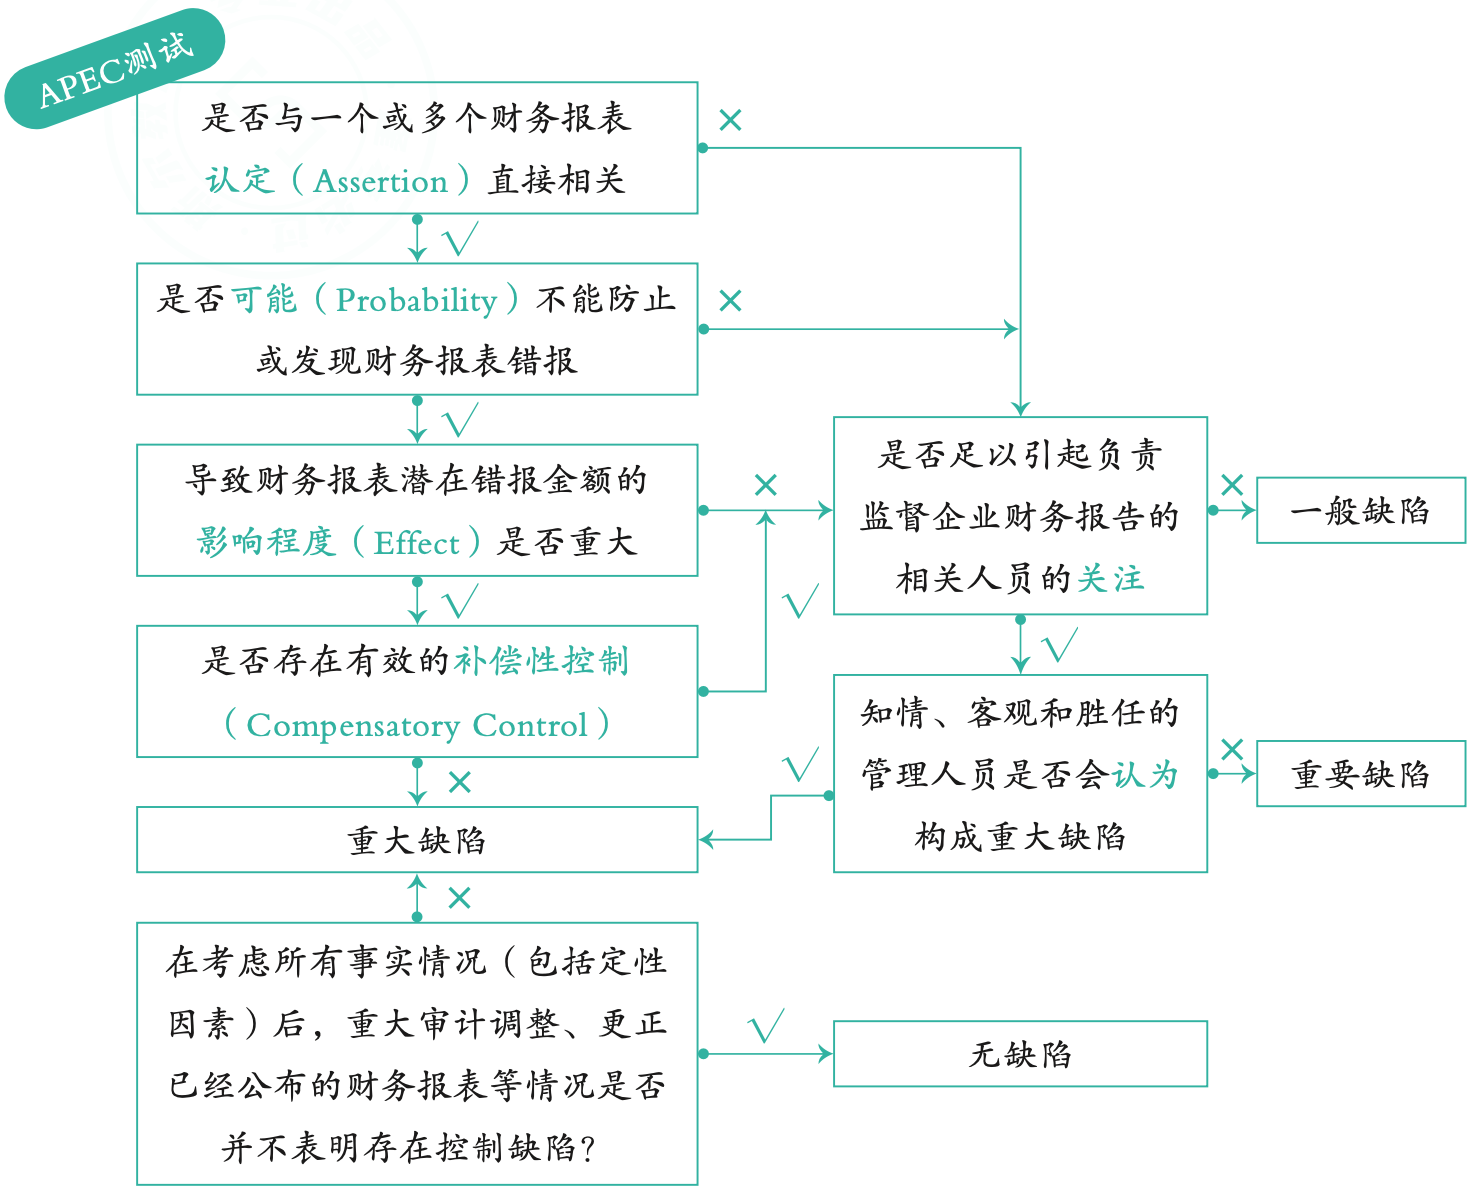
\includegraphics[width=0.7\linewidth]{pic/APECtest}
		\caption{}
		\label{fig:apectest}
	\end{figure}
	
	以下迹象表明可能存在重大缺陷
	\begin{enumerate}
		\item 注册会计师发现董事、监事和高级管理人员的任何舞弊 
		
		\item 被审计单位重述以前公布的财务报表,以更正由于舞弊或错误导致的重大错报 
		
		\item 注册会计师发现当期财务报表存在重大错报,而被审计单位内部控制在运行过程 中未能发现该错报
		
		\item 审计委员会和内部审计机构对内部控制的监督无效
	\end{enumerate}
	
	如果被审计单位在基准日前对存在缺陷的控制进行整改,整改后的控制需要运行足够长的时间,才能使注册会计师得出其是否有效的审计结论

	\subsection{内部控制审计报告}
	审计报告意见类型和普通的财务报表审计存在不同,没有保留意见
	
	如果认为内部控制存在一项或多项重大缺陷,除非审计范围受到限制,注 册会计师应当对内部控制发表否定意见
	
	在以下情况下发表无法表示意见
	\begin{enumerate}
		\item 如果审计范围受到限制,注册会计师应当解除业务约定或出具无法表示意见的内部控制审计报告
		
		\item 如果法律法规的相关豁免规定允许被审计单位不将某 些实体纳入内部控制的评价范围,注册会计师可以不 将这些实体纳入内部控制审计的范围,这种情况不构 成审计范围受到限制,但应当在内部控制审计报告中 增加强调事项段,或者在注册会计师的责任段中作出 恰当陈述
	\end{enumerate}

	在描述时,注册会计师不应在内部控制审计报告中指明所执行的 程序,也不应描述内部控制审计的特征,以避免产生 误解。如果在已执行的有限程序中发现内部控制存在重大缺 陷,注册会计师应当在内部控制审计报告中对重大缺 陷做出详细说明
	
	此外内部控制审计审计报告还有强调事项段和非财务报告内部控制重大缺陷描述段。这两者都不影响内部控制审计意见的发表。
	
	强调段主要包含以下内容
	\begin{enumerate}
		\item 企业内部控制评价报告对要素的列报不完整或不恰当
		
		\item 注册会计师知悉在基准日并不存在、但在期后期间发生的事项,且这类期后事项对内部控制有重大影响
	\end{enumerate}
	
	\newpage
	\section{会计师事务所业务质量管理}
	
	\subsection{会计师事务所质量管理体系}
	质量管理体系的总体要求是在全所(包含分所)范围内统一设计、实施和运行。以风险导向的思路“量身定制”,不断优化和完善。
	
	质量管理体 系的八要素如下
	\begin{enumerate}
		\item 会计师事务所的风险评估程序
		
		\item 治理和领导层
		
		\item 相关职业道德要求
		
		\item 客户关系和具体业务的接受与保持
		
		\item 业务执行
		
		\item 资源
		
		\item 信息与沟通
		
		\item 监控和整改程序
	\end{enumerate}
	
	会计师事务所主要负责人应当代表会计师事务所对质量管理体系进行评价。这种评价应当以某一时点为基准,并且应当至少每年一次
	
	会计师事务所应当规定质量管理体系工作记录的保存期限,该期限应当涵盖 足够长的期间,以使会计师事务所能够监控质量管理体系的设计、实施和运 行情况
	
	\subsection{项目质量复核}
	项目质量复核的人员应当在全所范围内(包括分所或分部)统一委派项目质量复核人员,并确保负责实施委派工作的人员具有必要的胜任能力和权威性。负责委派项目质量复核人员的人员需要独立于项目组(项目合伙人和项目组其他成员不得成为本项目的项目质量复核人员)
	
	复核的程序如下
	\begin{enumerate}
		\item 阅读并了解相关信息
		
		\item 与项目合伙人及项目组其他成员讨论重大事项及重大判断
		
		\item 选取部分与项目组作出的重大判断相关的业务工作底稿进行复核
		
		\item 评价项目合伙人确定独立性要求已得到遵守的依据
		
		\item 评价是否已就疑难问题或争议事项、涉及意见分歧的事项进行适当咨询,并评价咨询得出的结论
		
		\item 评价项目合伙人得出下列结论的依据
		
		\item 复核审计财务报表和审计报告
	\end{enumerate}
	
	如果项目质量复核人员怀疑项目组作出的重大判断或据此得出的结论不恰当,应当告知 项目合伙人;如果这一怀疑不能得到满意的解决,项目质量复核人员应当通知会计师事 务所适当人员项目质量复核无法完成 
	
	如果项目质量复核人员确定项目质量复核已经完成,应当签字确认并通知项目合伙人 
	
	项目合伙人禁止在收到项目质量复核人员就已完成项目质量复核发出的通知之前签署业 务报告
	
	\subsection{对财务报表审计实施的质量管理}
	项目合伙人应当对管理和实现审计项目的高质量承担总体责任
	
	在签署审计报告之前,审计项目合伙人应当负责确定相关职业道德要求(包括独立性要求)已经得到遵守
	
	审计项目合伙人应当确定会计师事务所就客户关系和审计业 务的接受与保持制定的政策和程序已得到遵守,并且得出的 相关结论是适当的
	
	复核工作底稿主要关注以下几项
	\begin{enumerate}
		\item 重大事项
		
		\item 重大判断,包括与在审计中遇到的困难或有争议事项相关的判断,以及得出的结论
		
		\item 根据审计项目合伙人的职业判断,与审计项目合伙人的职责有关的其他事项
	\end{enumerate}
	
	\newpage
	\section{职业道德基本原则和概念框架}
	职业道德基本原则有如下几个
	\begin{enumerate}
		\item 诚信
		
		\item 客观公正
		
		\item 独立性
		
		\item 专业胜任能力和勤勉尽责
		
		\item 保密
		
		\item 良好职业行为
	\end{enumerate}
	
	识别对职业道德基本原则的不利影响因素主要有以下几种
	\begin{enumerate}
		\item 自身利益
		\begin{enumerate}
			\item 在客户中拥有直接经济利益
			
			\item 会计师事务所的收入过分依赖某一客户
			
			\item 会计师事务所以较低的报价获得新业务,可能导致难以按照适用的职业准则要求执行业务
			
			\item 注册会计师与客户之间存在密切的商业关系
			
			\item 注册会计师能够接触到涉密信息,其可能被用于谋取个人私利
			
			\item 在评价所在会计师事务所以往提供的专业服务时,发现了重大错误
		\end{enumerate}
		
		\item 自我评价
		\begin{enumerate}
			\item 在对客户提供财务系统的设计或实施服务后,又对系统的运行有效性出具鉴证报吿
			
			\item 为客户编制用于生成有关记录的原始数据,而这些记录是鉴证业务的对象
		\end{enumerate}
		
		\item 过度推介
		\begin{enumerate}
			\item 推介客户的产品、股份或其他利益
			
			\item 当客户与第三方发生诉讼或纠纷时,为其辩护
			
			\item 站在客户的立场上影响某项法律法规的制定
		\end{enumerate}
		
		\item 密切关系
		\begin{enumerate}
			\item 审计项目团队成员的近亲属担任审计客户的董事或高级管理人员
			
			\item 鉴证客户的董高特,最近曾担任所在会计师事务所的项目合伙人
			
			\item 审计项目团队成员与审计客户之间存在长期业务关系
		\end{enumerate}
		
		\item 外在压力
		\begin{enumerate}
			\item 因对专业事项持有不同意见,受到客户解除业务关系或被会计师事务所解雇的威胁
			
			\item 因客户更具有专长,面临服从该客户判断的压力
			
			\item 除非其同意审计客户某项不恰当的会计处理,否则计划中的晋升将受到影响
			
			\item 接受客户赠予的重要礼品,被威胁将公开其收受礼品的事情
		\end{enumerate}
	\end{enumerate}
	
	
	\newpage
	
	\section{审计业务对独立性的要求}
	
	\subsection{基本概念和要求}
	近亲属包括主要近亲属(子女、父母、配偶)和其他近亲属(祖父母、外祖父母、孙子女、外孙子女、兄弟姐妹)
	
	公众利益实体包括
	\begin{enumerate}
		\item 上市公司
		
		\item 法律法规界定的公众利益实体
		
		\item 法律法规规定按照上市公司审计独立性的要求接受审计的实体
	\end{enumerate}

	对于上市公司,关联实体包括
	\begin{enumerate}
		\item 控股股东
		
		\item 重要投资人
		
		\item 合并范围内子公司
		
		\item 合并层面重要联营企业
		
		\item 姐妹实体
	\end{enumerate}
	对于非上市公司, 合并范围内子公司为关联实体
	
	
	\subsection{经济利益}
	经济利益可以分为直接经济利益和间接经济利益。以下人员不得在审计客户中拥有\textbf{直接经济利益}或\textbf{重大间接经济利益}
	\begin{enumerate}
		\item 会计师事务所、审计项目团队成员及其主要近亲属
		
		\item 与执行审计业务的项目合伙人同处一个分部的其他合伙人及其主要近亲属 
		
		\item 为审计客户提供非审计服务的其他合伙人、管理人员及其主要近亲属
	\end{enumerate}
	
	经济利益相关的其他情形
	\begin{enumerate}
		\item 与审计客户拥有共同经济利益:除非满足下列条件之一,否则不得在该实体中拥有经济利益经济利益  
		对会计师事务所、审计项目团队成员及其主要近亲属,以及审计客户  均不重要 
		审计客户无法对该实体施加重大影响
		
		\item 与审计客户的利益相关者(董、高、所有者)同时在某一实体拥有经济利益:可能因自身利益、密 切关系或外在压力产生不利影响
		
		\item 无意中获取的经济利益   通过继承、馈赠或因企业合并或类似情况,从审计客户获得直接经济利益 或重大间接经济利益
		项目组团队或其主要近亲属获得经济利益a. 立即处置 全部经济利益b. 立即处置 全部直接经济利益并处置足够数量的间接经济利益 
		
		项目组团队外的成员或其主要近亲属获得经济利益a. 在合理期限内尽快处置 全部经济利益b. 在合理期限内尽快处置 全部直接经济利益并处置足够数量的间接经济利益
		
		\item 对审计项目团队成员其他近亲属拥有经济利益的要求:拥有的直接经济利益或重大间接经济利益,将因自身利益产生非常严重的不利影响
		
		\item 对其他人员(会计师事务所合伙人、专业人员,两者的主要近亲属、与审计项目团队成员存在密切 私人关系的人员)拥有经济利益的要求   可能因自身利益对独立性产生不利影响
		
		\item 会计师事务所的退休金计划   通过退休金计划,在审计客户中拥有直接经济利益或重大间接经济利 益,可能因自身利益产生不利影响
	\end{enumerate}
	
	
	\subsection{贷款和担保以及商业关系、家庭和私人关系}
	\paragraph{贷款和担保}
	从银行或类似金融机构等审计客户取得
	除非该贷款或担保是按照正常的程序、条款和条件进行的,会计师事务所、审 计项目团队成员或其主要近亲属不得从银行或类似金融机构等审计客户取得贷 款,或获得贷款担保
	
	从不属于银行或类似金融机构等审计客户取得 
	会计师事务所、审计项目团队成员或其主要近亲属不得从不属于银行或类似金 融机构的审计客户取得贷款,或由此类审计客户提供贷款担保 
	
	向审计客户提供贷款或为其提供担保 
	会计师事务所、审计项目团队成员或其主要近亲属不得向审计客户提供贷款或 担保
	
	在审计客户开立存款或经纪账户 
	除非该存款或经纪账户是按照正常的商业条件开立的,会计师事务所、审计项 目团队成员或其主要近亲属不得在银行或类似金融机构等审计客户开立存款或 经纪账户
	
	\paragraph{商业关系}
	共同开办、捆绑 销售、互相推广
	会计师事务所、审计项目团队成员  不得与审计客户或
	其高级管理人员建立密切的商业关系
	审计项目团队成员的主要近亲属  应当评价不利影响的
	严重程度,并在必要时采取防范措施消除不利影响或将其
	降低至可接受的水平
	
	
	从审计客户购 买商品或服务
	按照正常的商业程序公平交易且性质不特殊、金额不重 大 通常不会对独立性产生不利影响 交易性质特殊或金额较大 可能因自身利益产生不利影响
	
	\paragraph{家庭和私人关系}
	为审计客户董高特,将对独立性产生非常严重的不利影响, 拥有此类关系的人员不得成为审计项目团队成员 在审计客户中所处职位能够对客户的财务状况、经营成果 和现金流量施加重大影响,可能因自身利益、密切关系或 外在压力对独立性产生不利影响
	
	审计项目团队成员的其他近亲属    为审计客户董高特,将因自身利益、密切 关系或外在压力对独立性产生不利影响
	
	审计项目团队成员的其他密切关系    与审计客户的员工存在密切关系,并且 该员工为审计客户的董高特,也将对独立性产生不利影响
	
	审计项目团队成员以外人员的家庭和私人关系    团队以外的合伙人或员工, 与审计客户的董高特之间存在家庭或私人关系,可能因自身利益、密切关系或外 在压力产生不利影响
	
	\subsection{与审计客户发生人员交流}
	
	\paragraph{与审计客户 发生雇佣关系}
	审计项目团队前任成员或前任合伙人担任审计客户的重要职位且与事务所保持重要联系    产生非常严重的不利影响,除非同时满足 该人员无权从会计师事务所获取报酬或福利 应付该人员的金额(如有)对会计师事务所不重要 该人员未继续参与,并且在外界看来未参与会计师事务所的经营活动或职业活动
	
	前任合伙人加入某一实体成为审计客户    加入某一实体并担任董高特,可 能因密切关系或外在压力对独立性产生不利影响 
	
	审计项目团队某成员拟加入审计客户    会计师事务所应当制定政策和程序, 要求审计项目团队成员在与审计客户协商受雇于该客户时,向其报告 
	
	关键审计合伙人加入属于公众利益实体审计客户担任重要职位(董高特)
	除非该合伙人不再担任该公众利益实体的关键审计合伙人后,该公众利益实体 发布的已审计财务报表涵盖期间不少于 12 个月,并且该合伙人未参与该财务 报表的审计,否则独立性将视为受到损害
	
	前任高级合伙人加入属于公众利益实体审计客户担任重要职位(董高特) 除非该高级合伙人不再担任该职位已超过 12 个月,否则独立性将被视为受到 损害
	
	\paragraph{向审计 客户借 出员工}
	可能因自我评价、过度推介或密切关系产生不利影响,除非同时满足下列条件

	仅在短期内向客户借出员工
	不参与注册会计师职业道德守则禁止提供的非鉴证服务
	不承担审计客户的管理层职责
	
	\paragraph{审计项目团队成员最近曾担任审计客户的董高特}
	在审计报告涵盖的期间不得将此类人员分派到审计项目团队
	
	会计师事务所的合伙人或员工不得兼任客户的董事或高级管理人员
	
	\subsection{与审计客户长期存在业务关系}
	\paragraph{已成为公众利益实体的审计客户的机制}
	担任项目合伙人、项目质量复核人员、其他属于关键审计合伙人 的职务不得超过五年(在任期内,如果某人员担任项目合伙人,不得在二年内担任该审计业务的项目质量复核人员)
		
	单一职务的冷静期
	\begin{enumerate}
		\item 担任单一职务的冷却期 担任项目合伙人累计达到五年 应当为连续五年
		
		\item 担任项目质量复核人员累计达到五年 应当为连续三年
		
		\item 担任其他关键审计合伙人累计达到五年 应当为连续二年
	\end{enumerate}
	
	\begin{enumerate}
		\item 担任项目合伙人累计达到三年或以上  应当为连续五年
		
		\item 担任项目质量复核人员累计达到三年或以上    应为连续三年 
		
		\item 担任项目合伙人和项目质量复核人员累计达到三年或以上,但累 计担任项目合伙人未达到三年    应当为连续三年 
		
		\item 不符合上述各项情况    应当为连续二年
	\end{enumerate}
	
	
	\paragraph{客户成为公众利益实体后的轮换机制}
	关于继续任职期 应当考虑,在该客户成为公众利益实体之前,该合伙人作为关键审计合伙人已为该客户提供服务的时间
	
	不超过三年  可继续提供服务五年减去已经服务的年限
	
	四年或更长的时间  最多还可以继续服务二年
	
	如客户是首次公开发行证券  不得超过二个完整会计年度
	
	\subsection{为审计客户提供非鉴证服务}
	\begin{enumerate}
		\item 承担管理层职责 会计师事务所承担审计客户的管理层职责,将因自身利益、自我评价、密切关系、过度推介对独立性产生非常严重的不利影响,不得承担审计客户的管理层职责
		
		\item 会计和记账服务。不对独立性产生不利影响的活动包括:沟通审计相关的事项、提供会计咨询服务(不承担审计客户的管理层职责)、日常性或机械性的会计和记账服务
		
		\item 行政事务性服务。向审计客户提供行政事务性服务(文字处理服务、编制行政或法定表格供客户 审批等)通常不会对独立性产生不利影响
		
		\item 评估服务。
		评估结果涉及高度的主观性,且评估服务对被审计财务报表具有重大影响,会计师 事务所不得向审计客户提供这种评估服务 
		
		评估服务经税务机关或类似监管机构外部复核,则通常不对独立性产生不利影响
		
		\item 税务服务。协助解决税务纠纷
		在公开审理或仲裁的税务纠纷中  担任审计客户的辩护人,并 且所涉金额对被审计财务报表具有重大影响  ,会计师事务所 不得向审计客户提供涉及协助解决税务纠纷的税务服务 在公开审理或仲裁期间,会计师事务所可以继续为审计客户 提供有关法庭裁决事项的咨询(提供背景材料或证词等)
		
		\item 内部 审计服务。在审计客户属于公众利益实体的情况下,会 计师事务所不得提供有关的内部审计服务
		财务报告内部控制的组成部分 财务会计系统 单独或累积起来对被审计财务报表 具有重大影响的金额或披露
		
		\item 信息技术系统服务。会计师事务所不得向属于公众利益实体的审计客户提供或设计与实施信息技
		术系统相关的服务
		信息技术系统构成财务报告内部控制的重要组成部分
		信息技术系统生成的信息对会计记录或被审计财务报表影响重大
		
		\item 诉讼支持服务。向审计客户提供诉讼支持服务,可能因自我评价或过度推介产生不利影响
		
		\item 法律服务。 向审计客户提供法律咨询服务,可能因自我评价或过度推介对独立性产生不利影响
		
		\item 招聘服务。如果属于审计客户拟招聘董高特,会计师事务所不得提供下列招聘服务:寻找或筛 选候选人;对候选人实施背景调查
		2 只要会计师事务所人员不承担管理层职责,下列服务通常不会对独立性产生不利影响 对多名候选人的专业资格进行审核,并就其是否适合该职位提供咨询意见 对候选人进行面试,并对候选人在财务会计、行政管理或内部控制等职位上的胜任 能力提供咨询意见
		
		\item 公司财务服务。会计师事务所提供财务服务,可能因自我评价或过度推介对独立性产生不利影响
	\end{enumerate}
	
	\subsection{影响独立性的其他事顶}
	会计师事务所在提供审计服务时,以直接或间接形式取得\textbf{或有收费},将因自身利益产生非常严 重的不利影响,不得采用这种收费安排
	
	接受审计客户的礼品,将产生非常严重的不利影响,不得接受礼品
	 
	应当评价接受款待产生不利影响的严重程度,考虑款待是否具有不当影响注册会计师行为的意图
	
\end{document}